\documentclass[11pt]{amsart}
\usepackage[T1]{fontenc}
\usepackage{lmodern,amsmath,amssymb,amsthm,mathtools,microtype,booktabs,array,longtable}
\usepackage[margin=1.06in]{geometry}
\usepackage{tikz}
\usepackage[hidelinks]{hyperref}
\hypersetup{pdftitle={Finite-Use Geometry and Learning of Ordered Quantum Measurements},pdfauthor={Qian Qi}}
\emergencystretch=2em
\numberwithin{equation}{section}
\newtheorem{theorem}{Theorem}[section]
\newtheorem{lemma}[theorem]{Lemma}
\newtheorem{proposition}[theorem]{Proposition}
\newtheorem{corollary}[theorem]{Corollary}
\theoremstyle{definition}\newtheorem{definition}[theorem]{Definition}
\theoremstyle{remark}\newtheorem{remark}[theorem]{Remark}
\newcommand{\Q}{\mathbb Q}\newcommand{\R}{\mathbb R}\newcommand{\C}{\mathbb C}\newcommand{\N}{\mathbb N}\newcommand{\Z}{\mathbb Z}\newcommand{\E}{\mathbb E}
\newcommand{\ip}[2]{\langle #1,#2\rangle}\newcommand{\norm}[1]{\lVert #1\rVert}
\newcommand{\epsc}{\varepsilon_{\mathrm c}}
\DeclareMathOperator{\osc}{osc}\DeclareMathOperator{\spanop}{span}\DeclareMathOperator{\End}{End}\DeclareMathOperator{\diag}{diag}\DeclareMathOperator{\tr}{tr}\DeclareMathOperator{\rad}{rad}\DeclareMathOperator{\TV}{TV}
\title[Finite-use measurement geometry and learning]{Finite-Use Geometry and Learning of Ordered Quantum Measurements}
\author{Qian Qi}
\date{5 October 2026}
\subjclass[2020]{Primary 81P15, 81P47; Secondary 94A17, 81P70}
\begin{document}
\raggedbottom
\begin{abstract}
We study memoryless quantum measurements that consume their input and
return an ordered classical label, with no residual quantum system.
On the complete binary effect body, a regularized midpoint Sylvester
form compares finite-use adaptive distinguishability, including all
spectral boundaries.  At fixed input dimension $d$, the small-error
covering order is
$N^{d^2/2}[\log(N+2)]^{\lfloor d/2\rfloor}\delta^{-d^2}$.
Common learning and finite exact coding attain matching
fixed-dimensional resource orders; the full-body learner has an
explicit $d^4$ upper factor.

For every fixed finite outcome count $k$, we establish a second
joint theory on the balanced interior
$\sum_jE_j=I_d$, $I_d/(2k)\preceq E_j\preceq3I_d/(2k)$,
without commutation assumptions.  A horizontal matrix differential
equation gives dimension-independent comparison with
$\sqrt N\max_j\|E_j-F_j\|_{\rm op}$.
The entropy is
$((k-1)d^2/2)\log_2N+(k-1)d^2\log_2(1/\delta)+O_k(d^2)$.
The minimax training order is
$\Theta_k(N\delta^{-2}[d^2+d\log(1/\eta)])$,
jointly in dimension, horizon, accuracy, and confidence.
Independent one-call Choi acquisitions attain the upper bound;
the converse allows arbitrary coherent adaptive training.
A finite rational construction attains this query order and the
optimal-order public description length simultaneously.
Finite net inequalities certify uniform risk on every real target,
with an explicit continuity allowance.
The joint learning statement holds for $d,N\ge1$,
$0<\delta\le2^{-24}$ and $0<\eta\le1/8$; effective synthesis uses
rational accuracy and confidence.  Full-body and binary-interior
results retain their original wider ranges.  Reconstruction time,
workspace, and finite trusted-control costs are distinguished from
unknown-device calls and transmitted bits.
\end{abstract}
\maketitle
\section{Introduction}

We study the finite-use geometry of input-consuming quantum
measurements with ordered classical outputs and no residual quantum
system.  There are two complementary parameter families: the complete
body of binary effects, including singular boundaries, and balanced
interiors of arbitrary finite outcome alphabets.  In the second family
no simultaneous diagonalization is assumed.  The results join
operational comparison, description entropy, common learning, and
finite exact realization under one declared interface.

Repeated uses of an ordered binary quantum measurement resolve
different perturbations at different scales.  An interior change of
an eigenvalue is detected at scale $N^{-1/2}$, whereas a rotation of
a projective measurement can be detected at scale $N^{-1}$.  These
scales meet at singular effects and repeated eigenvalues.  We
determine the resulting geometry on the compact body of matrix
effects, calculate its description entropy, and construct common
learners whose loss is distinguishability by all future experiments
with at most $N$ uses.

For an input dimension $d$, let
\[
 \mathfrak E_d=\{E=E^*\in M_d(\C):0\preceq E\preceq I_d\}.
\]
An effect $E$ specifies the memoryless ordered binary measurement
\[
 \mathcal M_E(\rho)=\operatorname{tr}(E\rho)|1\rangle\langle1|
       +\operatorname{tr}((I_d-E)\rho)|0\rangle\langle0|.
\]
The input is consumed; the device returns a classical outcome and
no residual quantum system.  The distance $d_N$ is the supremum
of the unhalved trace norm between the final states of a common
experiment with at most $N$ calls.  Such an experiment may entangle
inputs, retain an arbitrary reference and quantum memory, use
feedback, and stop at a public bounded time.  Thus $0\le d_N\le2$;
classical total variation is one half of the corresponding trace
norm.  The nonadaptive restriction $d_N^{\rm na}$ allows entangled
input blocks and retained references, without feedback between calls.

\subsection{Geometry and entropy of the closed effect body}
For $E,F\in\mathfrak E_d$, put
\[
 M=\tfrac12(E+F),\qquad H=F-E,\qquad V=M(I_d-M),
\]
and define the comparison modulus
\[
 Q_N(E,F)^2=N\langle H,
       (L_V+R_V+N^{-1}\operatorname{Id})^{-1}H\rangle_{\rm HS}.
\]
The inverse acts on the real Hilbert space of Hermitian matrices.
For every $d,N\ge1$, Theorem~\ref{thm:matrixmetric76} gives
\begin{equation}\label{eq:intrometric77}
 \frac{\min\{1,Q_N(E,F)\}}{8192d}
 \le d_N^{\rm na}(\mathcal M_E,\mathcal M_F)
 \le d_N(\mathcal M_E,\mathcal M_F)
 \le\min\{2,8Q_N(E,F)\}.
\end{equation}
The comparison holds at every spectral rank and multiplicity, with
no margin from the support endpoints.  In particular,
$d_N\le65536d\,d_N^{\rm na}$ uniformly in $N$.  The modulus
provides an explicit comparison of the operational distances;
its use requires no triangle inequality for $Q_N$.

A horizontal measurement dilation gives the adaptive tangent bound.
A regularized Sylvester equation separates the tangent into a
horizontal part and a remainder controlled by the hybrid inequality.
Operator concavity of $G(I_d-G)$ then integrates the bound along
a finite segment, including boundary endpoints.  Bernoulli inputs
and exact two-dimensional compressions give the converse.  These
pair-dependent experiments establish separation; the common
learning construction below is a separate argument.

Let $\mathcal C_N(\mathfrak E_d,\delta)$ be the least number of
legal memoryless binary centres in a $d_N$-cover.  For every fixed
$d$, Theorem~\ref{thm:matrixcover76} proves
\begin{equation}\label{eq:introentropy77}
 \mathcal C_N(\mathfrak E_d,\delta)
 \asymp_d N^{d^2/2}[\log(N+2)]^{\lfloor d/2\rfloor}\delta^{-d^2},
 \qquad N\ge1,\quad0<\delta\le\delta_d.
\end{equation}
The positive cap $\delta_d$ and comparison constants may depend
on $d$.  The proof bounds the weighted volume of actual operational
balls uniformly over all boundary strata.  The total volume is a
spectral integral: its ordered endpoint sectors have cumulative
exponents $S_j^2/2$, where $S_j$ is a signed prefix sum.  Balanced
prefixes, together with matching nested endpoint boxes, give the
logarithmic multiplicity $\lfloor d/2\rfloor$.

\subsection{Common learning and independent acquisition blocks}
The learner receives calls to an unknown effect, without its matrix
entries.  Theorem~\ref{thm:matrixlearning77} constructs one procedure
common to all $E\in\mathfrak E_d$ such that
\begin{equation}\label{eq:introlearning77}
 \sup_E\mathbb P_E\{d_N(\mathcal M_E,\mathcal M_{\widehat E})
                         >\delta\}\le\eta,
 \qquad
 M\le Cd^4N\delta^{-2}\log(d/\eta),
\end{equation}
where $C$ is absolute, $N\ge1$, $0<\delta\le\delta_0$ for an
absolute $\delta_0>0$, and $0<\eta\le1/8$.  The training-call
bound holds on every record, and each entangled block uses at most
$N$ calls.  A scalar Bernoulli subfamily gives a lower bound of
order $N\delta^{-2}\log(1/\eta)$ even for arbitrary
reference-assisted adaptive training.  Thus the horizon, accuracy,
and confidence orders are optimal for fixed $d$; the displayed
$d^4$ factor is an upper bound.

The qubit construction learns unknown bias, contrast, and direction.
Independent fair signs remove the bias from GHZ parity observations.
A dyadic amplitude search maintains a small-cone invariant and
terminates at the first rejected scale.  Fresh observations after
each data-dependent choice complete the direction and endpoint
estimates.  Conditional confidence allocation controls exceptional
records as well as the maximum training cost.

The matrix extension first calibrates both support boundaries in
relative Loewner order at scale $N^{-1}$ and the absolute matrix
error at scale $N^{-1/2}$.  In the calibrated eigenbasis, these
estimates control the additional variance produced by every
two-dimensional compression.  Qubit learning on the compressions
then supplies compatible coordinates in the regularized quadratic
form.  Projection onto the legal effect body, followed by rational
selection, completes the estimate.  Conditional summation of the
calibration and compression budgets introduces no $\log N$ factor.

The maximal independent block length is a further acquisition
resource.  Within a fresh block, reference-assisted quantum controls
are allowed.  At its boundary, completed outputs may be processed
jointly, and the classical record may determine the next preparation.
The next block, including its reference and unused inputs, is
isolated from earlier quantum registers until its final call.
Thus collective final estimation and classical feedback are allowed,
while older quantum memory cannot feed unfinished queries.

For a declared cap $1\le b\le N$ and every fixed $d\ge2$,
Theorem~\ref{thm:blocklearning78} proves
\begin{equation}\label{eq:introblock78}
 M_b^\star(d,N,\delta,\eta)
 =\Theta_d\!\left(\frac{N^2}{b\delta^2}\log\frac1\eta\right)
\end{equation}
for an absolute small-error range and $0<\eta\le1/8$.  The
explicit upper bound is
\[
 Cd^4(N^2/b)\delta^{-2}\log(d/\eta).
\]
Horizon blocking gives the common learner; a history-weighted
root-fidelity bound gives the converse with arbitrary storage and
collective processing of completed blocks.  In dimension one the
device is a coin, and the cost is
$\Theta(N\delta^{-2}\log(1/\eta))$ for every $b$.

\subsection{Joint learning laws in the interior}
On the full-dimensional interior
\[
 \mathfrak I_d=\{E:I_d/4\preceq E\preceq3I_d/4\},
\]
the operational distance has a dimension-free comparison with
$\min\{1,\sqrt N\|E-F\|_{\rm op}\}$.  The binary Choi estimator
of Mele--Bittel \cite{MB67}, analysed under this loss, gives
\begin{equation}\label{eq:introinterior78}
 M_{\rm int}^\star(d,N,\delta,1/8)
 =\Theta(d^2N\delta^{-2})
\end{equation}
with absolute constants, using independent one-call probes.  For
the converse, a family within operator radius $r$ of $I/2$
supplies at most $4r^2$ information about its finite unknown label
per call.  Matrix packing and Fano's inequality give
Theorem~\ref{thm:dimensionlower78}, which permits arbitrary coherent
adaptive training.

The confidence dependence is also determined jointly.  For all
$d,N\ge1$, $0<\delta\le2^{-13}$ and $0<\eta\le1/8$,
Theorem~\ref{thm:interiorconfidence80} proves
\begin{equation}\label{eq:introconfidence80}
 M_{\rm int}^{\star}(d,N,\delta,\eta)
 =\Theta\!\left(\frac{N}{\delta^2}
                   \left(d^2+d\log\frac1\eta\right)\right).
\end{equation}
The constants are absolute.  The upper bound uses independent
one-call Choi acquisitions, and the lower bound allows coherent
adaptive training; hence the order is the same under every
fresh-block cap.  At $N=1$ it gives the joint dimension, accuracy,
and confidence law for binary operator-norm learning, including
the fixed-confidence order $\Theta(d^2\epsilon^{-2})$.

The confidence converse compares $I_d/2$ with $d$ diagonal
single-coordinate perturbations.  Revealing the sampled basis
index gives a relative-entropy chain rule through retained quantum
memory.  Under the central hypothesis, the expected occupation
counts sum to the entire budget, so binary testing forces the
$d\log(1/\eta)$ term.  Taking the maximum with the packing
bound gives the sum in \eqref{eq:introconfidence80} up to an
absolute factor.  For the upper bound, the estimator of
\cite[Corollary~III.9]{MB67} is run at a rational failure
probability exponentially small in $d$.  Independent repetition
and metric-majority selection give the required confidence at the
same additive cost.

The resulting operator estimator also applies to the closed body.
At operator accuracy $\delta/(2N)$, the hybrid inequality gives
future loss at most $\delta$.  Selection between this one-call
procedure and the block learner, using only public parameters,
yields
\[
 M_b^\star\le C\frac{N^2}{\delta^2}
 \min\left\{d^2+d\log(1/\eta),\frac{d^4}{b}\log(d/\eta)\right\}
\]
in their common range; see
\eqref{eq:fullbodyconfidenceupper80}.  The corresponding joint
lower obstructions are given in
\eqref{eq:fullbodyconfidencelower80}.  In particular, the projective
boundary in \eqref{eq:introblock78} accounts for the different
horizon cost of one-call acquisition on the closed body.

\subsection{Exact descriptions and learned words}
Theorem~\ref{thm:matrixcodec77} constructs a deterministic finite
rational codebook at the order in \eqref{eq:introentropy77}.
Exact comparisons of $Q_N^2$ define a greedy selection on a finite
legal matrix grid.  Separation in the actual operational metric
controls its cardinality, and inward rounding gives coverage at
every rank.  Encoder and decoder reconstruct the same dictionary
from public parameters; every fixed-length word decodes to a legal
effect.  Its payload is
\[
 \frac{d^2}{2}\log_2N+
 \lfloor d/2\rfloor\log_2\log(N+2)
             +d^2\log_2(1/\delta)+O_d(1).
\]
The direct qubit code also gives detailed resource bounds.
Corollary~\ref{cor:matrixlearnedcode77} combines the common learner
and exact encoder at their respective optimal fixed-dimensional
orders, without further device calls.
Corollary~\ref{cor:blocklearnedcode78} gives the same conclusion
under a prescribed independent-block cap.

The interior has a dimension-uniform description law.  For all
$d,N\ge1$ and $0<\delta\le2^{-13}$,
Theorem~\ref{thm:interiorentropy79} gives
\begin{equation}\label{eq:introinteriorentropy79}
 \left(\frac{\sqrt N}{2048\delta}\right)^{d^2}
 \le\mathcal C_N(\mathfrak I_d,\delta)
 \le\left(\frac{25\sqrt N}{\delta}\right)^{d^2}.
\end{equation}
The lower bound allows arbitrary legal binary centres.
Theorem~\ref{thm:interiorcodec79} realizes the upper bound by
finite exact rational comparison and public reconstruction.  With
\[
 A_d(N,\delta)=\tfrac12d^2\log_2N+d^2\log_2(1/\delta),
\]
its length is $A_d(N,\delta)+O(d^2)$, uniformly in all parameters;
there is no $d^2\log d$ entrywise-transmission penalty.  The
absence of the endpoint logarithm reflects the interior geometry.

With shared randomness and worst-target failure probability
$0\le\eta\le1/8$, Theorem~\ref{thm:prefixrate79} gives optimal
expected one-way prefix length
$(1-\eta)A_d(N,\delta)+O(d^2)$.  Its converse permits a
randomized decoder and counts all nonpublic information.  Its
upper bound uses a public target-independent abort event, whose
occurrence requires no transmitted flag.  For learned descriptions,
Theorem~\ref{thm:interiorlearnedcode79} attains the call order
in \eqref{eq:introinterior78} and this deterministic index length
at failure $1/8$; Corollary~\ref{cor:interiorconfidencecode80}
attains \eqref{eq:introconfidence80} at every stated confidence.

\subsection{Finite risk certificates and trusted controls}
For rational public errors, these joint query and description
orders admit a complete finite classical specification before the
first device call.  The algebraic construction in
Theorem~\ref{thm:effectiveinterior80} fixes the public dictionary
and a collective readout on independent Choi records.  The
subnormalized record is polynomial in the unknown effect, so
positivity, completeness, and uniform success form a first-order
formula over the reals with rational coefficients.  Effective
quantifier elimination decides feasibility, and algebraic-point
selection returns exact readout data.  The statistical existence
bound controls the first feasible call count.

Section~\ref{sec:finiterisk81} gives a rational construction with
finite certificates of uniform risk.  Theorem~\ref{thm:finitecertificate81}
transfers verified inequalities on a finite rational grid to every
real effect in $\mathfrak I_d$.  If the grid is an operator-norm
$r$-net, and its tests bound failure by $\alpha$ at operator
radius $a$, then an $m$-call readout satisfies
\[
 \sup_{E\in\mathfrak I_d}
   \mathbb P_E\{\|E-C_J\|_{\rm op}>a+r\}\le\alpha+mr.
\]
An analytic continuity bound for the complete Choi record proves
the transfer with one fixed set of good labels at each grid point.
The prescribed parameters certify operational loss $5\delta/8$
with failure at most $5\eta/16$.
Proposition~\ref{prop:rationalreadout81} supplies rational POVMs
with exact positivity and completeness while preserving the risk
margin.  Bounded-denominator enumeration and a doubling schedule
then give the computable learner of
Theorem~\ref{thm:rationallearner81}, with the call order in
\eqref{eq:introconfidence80} and payload
$A_d(N,\delta)+O(d^2)$.  This construction uses finite rational
tests in place of real quantifier elimination.

The finite-control theorem approximates trusted preparations and
readouts with a pathwise norm budget.  It preserves the operational
loss, confidence, and every-record call orders, and it charges
classical specifications and trusted realization errors explicitly.
The interior constructions retain fresh one-call acquisitions and
collective processing of completed outputs.  Exhaustive dictionary
reconstruction, readout synthesis, quantum storage, and known-control
work are separate resources from device calls and transmitted bits;
the finite constructions assert computability without an efficiency
bound for those resources.

\subsection{Antecedents and organization}
Horizontal Kraus gauges, channel-extension metrology, and integration
of local distinguishability underlie the path argument
\cite{FI76,DKG67,DM76,KGAD76,YF76,SD76}.  Inverse-Sylvester
geometry and spectral matrix integration have classical antecedents
\cite{Dittmann76,SZGeom76}.  Here these methods enter the explicit
closed-body midpoint comparison and the nested endpoint entropy.
Mele--Bittel \cite{MB67} and
Zambrano--Ramos-Calderer--Kueng \cite{ZRK76} provide common
estimators under one-use measurement losses.  Their precise access,
dimension, rank, and confidence statements, and the future-loss
analysis of those acquisitions, are compared in
Section~\ref{sec:matrixcomparison76}.  The phase-estimation
components of the full-body learner use ideas from
\cite{HB76,KLY76}, with the conditional construction proved here.

The matrix geometry and entropy precede the qubit learning
construction, its matrix extension, and the exact dictionary.
The independent-block theorem and the interior comparison then
lead to the joint learning, confidence, and description laws.
Finite-control synthesis and rational risk certification complete
the construction.  The subsequent qubit geometry and the final
prerequisite appendix provide the remaining proofs needed by the
article.


\subsection{A finite outcome alphabet}
For $k\ge2$ let $\mathfrak P_{d,k}$ consist of the ordered tuples
$\boldsymbol E=(E_1,\ldots,E_k)$ satisfying
$\sum_jE_j=I_d$ and $I_d/(2k)\preceq E_j\preceq3I_d/(2k)$.
Put $p=(k-1)d^2$ and
$r(\boldsymbol E,\boldsymbol F)=\max_j\|E_j-F_j\|_{\rm op}$.
Theorems~\ref{thm:multioutcomemetric82}--\ref{thm:multioutcomecode82}
give, with constants independent of the input dimension,
\[
 \frac1{128}\min\{1,\sqrt N r\}
 \le D_N^{\rm na}\le D_N\le\min\{2,2k\sqrt N r\},
\]
\[
 \log_2\mathcal C_{N,k}(\delta)
 =\frac p2\log_2N+p\log_2(1/\delta)+O(p\log(k+1)).
\]
The entropy statement holds for $0<\delta<1/128$ and allows arbitrary
legal decoding centres.  A rational inward grid preserves the sum of
all effects and both spectral inequalities.  An exact public code
attains the displayed length, with finite but unoptimized reconstruction.
The horizontal differential equation
$\dot X_j=X_j A_j^{-1}\dot A_j/2$ provides the upper geometry;
its cross-slot cancellation uses $\sum_j\dot A_j=0$ rather than
commutation.  A single-label Bernoulli test supplies the lower geometry.

For every fixed $k$, Theorem~\ref{thm:multioutcomelearning82} proves
\[
 M^*_{d,k}(N,\delta,\eta)
 =\Theta_k\!\left(N\delta^{-2}[d^2+d\log(1/\eta)]\right)
\]
jointly for $d,N\ge1$, $0<\delta\le2^{-24}$ and $0<\eta\le1/8$.
The explicit upper factor is $Ck^3$ with confidence logarithm
$\log(k/\eta)$; the lower constant is absolute.  Thus no optimal
claim in a growing outcome count is implicit.  Independent one-call
Choi preparations attain the upper bound, with a simultaneous
optimal-order fixed public index.  Public random relabeling reduces
each component to an interior binary learner.  Exact legalization
restores the common normalization.  Conversely, a label-splitting
embedding of binary effects transfers the coherent adaptive lower
bound, including its dimension-dependent confidence contribution.

Theorem~\ref{thm:multicertificate82} gives finite risk certificates
for collective $k$-outcome Choi records.  A complete tuple $r_0$-net
at radius $a$ and failure $\alpha$ transfers to every real target
at radius $a+r_0$ and failure $\alpha+Mk r_0/2$.
The statement uses a fixed set of successful output labels; no
continuity of the decision boundary is assumed.

These finite-outcome results concern the balanced interior, not the
full spectral boundary of arbitrary POVMs.  The complete binary-body
results and their endpoint logarithms remain unchanged.  Neither
family includes a device-returned postmeasurement quantum state.
The underlying one-use tomography primitive is credited to
Mele--Bittel; the transfer of its guarantees to the present future-use
loss, the matching coherent converse, and the explicit description
and certificate constructions are distinguished in the comparison
section.  Human specialist priority assessment, exact adaptive
optima, and algorithmically efficient synthesis are not consequences
of source reconstruction or finite arithmetic checks.

\section{Matrix geometry in arbitrary input dimension}
\label{sec:matrixmetric76}

The binary effect body has a finite-use description that does not
require eigenvector coordinates.  Its regularization is the same at
every spectral rank, and two-dimensional compressions supply lower
witnesses for the full matrix problem.  Throughout this section
$d,N\ge1$ are integers and
\begin{equation}\label{eq:matrixbody76}
 \mathfrak E_d=\{E\in\End(\C^d):E=E^*,\ 0\preceq E\preceq I_d\}.
\end{equation}
The measurement $\mathcal M_E$ has the ordered effects $E,I_d-E$
and no residual quantum output.  The distance $d_N$ has the same
reference-assisted adaptive meaning as in
Theorem~\ref{thm:biasedmetric75}.  Write $d_N^{\rm na}$ for its
restriction to nonadaptive experiments, allowing entanglement across
the calls and a retained reference.  These experiments may depend on
the known pair of hypotheses.

Put $\tau=N^{-1}$ and $V_E=E(I_d-E)$.  On the real Hilbert space
of Hermitian matrices with Hilbert--Schmidt inner product, define
\begin{align}
 \mathcal A_E(H)&=V_EH+HV_E+\tau H,
                                      \label{eq:matrixoperator76}\\
 g_{N,E}(H)^2&=N\ip{H}{\mathcal A_E^{-1}(H)}_{\rm HS}.
                                      \label{eq:matrixform76}
\end{align}
The operator $\mathcal A_E$ is strictly positive, including at a
singular effect.  For a pair $E,F$ set
\begin{equation}\label{eq:matrixmodulus76}
 M=\tfrac12(E+F),\qquad H=F-E,\qquad
 Q_N(E,F)=g_{N,M}(H).
\end{equation}
In any orthonormal eigenbasis of $M$, with eigenvalues $m_i$ and
$v_i=m_i(1-m_i)$, this is
\begin{equation}\label{eq:matrixcoordinates76}
 Q_N(E,F)^2=N\sum_{i,j=1}^d
                \frac{|H_{ij}|^2}{v_i+v_j+N^{-1}}.
\end{equation}
Definition~\eqref{eq:matrixmodulus76} makes the expression independent
of all choices at repeated eigenvalues.  We use it as a comparison
modulus; a triangle inequality for $Q_N$ is not required.

The inverse Sylvester operator is familiar from the Bures metric
$g^{\rm B}$ on the positive definite cone \cite{Dittmann76}.
Its normalization gives the algebraic identity
\[
 g_{N,E}(H)^2=2N\,g^{\rm B}_{V_E+\tau I_d/2}(H,H).
\]
Here $H$ remains the effect tangent; the differential of the
variance map $E\mapsto V_E$ is $H-EH-HE$.

\begin{theorem}[Finite-use geometry of the matrix effect body]
\label{thm:matrixmetric76}
For every $E,F\in\mathfrak E_d$,
\begin{equation}\label{eq:matrixmetric76}
 \frac1{8192d}\min\{1,Q_N(E,F)\}
 \le d_N^{\rm na}(\mathcal M_E,\mathcal M_F)
 \le d_N(\mathcal M_E,\mathcal M_F)
 \le\min\{2,8Q_N(E,F)\}.
\end{equation}
The constants are uniform in the horizon and in both effects,
without a spectral margin or a condition on eigenvalue multiplicities.
The adaptive upper bound permits arbitrary retained references,
common feedback, and bounded public stopping.  Each lower witness
uses inputs in one fixed subspace of dimension at most two.  Moreover,
\begin{equation}\label{eq:matrixoneuse76}
 d_1(\mathcal M_E,\mathcal M_F)=2\|E-F\|_{\rm op}.
\end{equation}
\end{theorem}

The theorem includes every rank of projection and all of the
intermediate singular strata.  The variance $E(I_d-E)$, rather than
the smallest eigenvalue of either outcome, determines the matrix
weights.  The factor $N^{-1}$ makes the formula finite on the entire
closed body.  The proof first establishes a path inequality valid for
every common adaptive tester, and then obtains the converse from
one- and two-dimensional experiments.

\subsection{A horizontal measurement dilation}

Kraus-gauge bounds for channel estimation were developed in
\cite{FI76,DKG67,DM76}.  Their integration along channel paths
appears in \cite[Section~III, equation~(26)]{YF76} and, with
general adaptive bounds, in \cite[Section~IV.A]{SD76}.  We use an
explicit horizontal lift for binary effects and control the
finite-horizon regularization by a trace-norm remainder.

\begin{lemma}[Horizontal derivative and regularized path bound]
\label{lem:matrixpath76}
Every continuously differentiable path $G:[0,1]\to\mathfrak E_d$
satisfies
\begin{equation}\label{eq:matrixpath76}
 d_N(\mathcal M_{G(0)},\mathcal M_{G(1)})
       \le4\int_0^1 g_{N,G(t)}(G'(t))\,dt.
\end{equation}
\end{lemma}
\begin{proof}
We begin with an interior effect $G$, so that $G$ and $I_d-G$
are invertible.  Set $S=\sqrt{G(I_d-G)}$.  For a Hermitian matrix
$K$ put $H_0=SK+KS$.  At the two factors
$A_1=\sqrt G$, $A_0=\sqrt{I_d-G}$ prescribe derivatives
\begin{equation}\label{eq:horizontalderivatives76}
 B_1=\sqrt{I_d-G}\,K,\qquad B_0=-\sqrt G\,K.
\end{equation}
They obey
\begin{align}
 A_1^*B_1+B_1^*A_1&=H_0,&
 A_0^*B_0+B_0^*A_0&=-H_0,\notag\\
 \sum_{y=0}^1 A_y^*B_y&=0,&
 \sum_{y=0}^1 B_y^*B_y&=K^2.
                                      \label{eq:horizontalidentities76}
\end{align}

These tangent equations can be realized by genuine dilations.
Let $G_1(s)=G+sH_0$, $G_0(s)=I_d-G-sH_0$ for $s$ in a
sufficiently small open interval, and put $R_y(s)=\sqrt{G_y(s)}$.
The first line of \eqref{eq:horizontalidentities76} implies that
\[
 T_y=(B_y-R_y'(0))R_y(0)^{-1}
\]
is anti-Hermitian.  Indeed, multiplying $T_y+T_y^*$ on the left
and right by $R_y(0)$ gives, with $R=R_y(0)$,
\[
 R(T_y+T_y^*)R=RB_y+B_y^*R-(RR_y'(0)+R_y'(0)R)=0,
\]
by differentiating $R_y(s)^2=G_y(s)$.  Thus
$\widetilde A_y(s)=\exp(sT_y)R_y(s)$ has derivative $B_y$ at
zero and satisfies
$\widetilde A_y(s)^*\widetilde A_y(s)=G_y(s)$ exactly.  A measurement
isometry is
\[
 W(s)\psi=\sum_{y=0}^1
              |y\rangle_C|y\rangle_L\widetilde A_y(s)\psi.
\]
Here $C$ is the observed outcome, and $L$ and the factor space of
$\widetilde A_y$ are environments.  Tracing the environments
implements $\mathcal M_{G(s)}$, also on inputs entangled with a
reference.  At zero, \eqref{eq:horizontalidentities76} gives
\begin{equation}\label{eq:horizontaloverlap76}
 W^*\dot W=0,\qquad \dot W^*\dot W=K^2.
\end{equation}

The horizontal Kraus condition has the antecedents
\cite[Theorems~4--5]{FI76}. Its adaptive channel-extension form is
$F_N\le4N\|\alpha\|$ when $\beta=0$; see
\cite[equation~(9)]{DM76} and \cite[equations~(5)--(10)]{KGAD76}.
In the present lift $\alpha=K^2$ and $\beta=0$. We give the cancellation
explicitly for this binary measurement.

Fix a common tester with $N$ slots.  Purify its initial state and
all intervening operations, and retain the measurement environments
only for this comparison; neither the outcome copy nor the factor
environment is accessible to the tester.  The derivative of its final purification
in the direction $H_0$ is the sum of $N$ terms, each having one
differentiated occurrence of $W$.  The terms are mutually orthogonal.
For two different differentiated slots, cancel the common isometries
after the later slot; the remaining overlap contains
$W^*\dot W\otimes I=0$.  Each term has norm at most
$\|\dot W\|_{\rm op}=\|K\|_{\rm op}$, independently of the
reference and memory dimensions.  Hence the derivative of the
purification has norm at most $\sqrt N\|K\|_{\rm op}$.
The pure-state trace-norm derivative bound, followed by contraction
under the partial trace, bounds the observed output derivative by
\begin{equation}\label{eq:horizontaltangent76}
 2\sqrt N\|K\|_{\rm op}.
\end{equation}
A publicly stopped tester is padded to $N$ slots by calls on fixed
dummy inputs, whose outcomes and environments are both discarded.  The same purification
argument then applies to its original output.  Classical feedback is
included by purifying the common controlled operations.

Now let $H$ be an arbitrary Hermitian tangent at $G$, and set
$\kappa=N^{-1/2}$.  There is a unique Hermitian solution of
\begin{equation}\label{eq:regularizedsylvester76}
 SK+KS+\kappa K=H.
\end{equation}
Write $H=H_0+R$, with $H_0=SK+KS$ and $R=\kappa K$.
Both are legitimate tangents at the interior effect $G$.  The
derivative of a fixed tester's output is linear in the inserted
channel tangent.  The part arising from $H_0$ is bounded by
\eqref{eq:horizontaltangent76}.  The part arising from $R$ is
bounded by $2N\|R\|_{\rm op}$.  To verify the latter bound,
the one-call tangent has two opposite reference blocks
\[
 B_\rho=\tr_A[(R\otimes I)\rho],\qquad -B_\rho.
\]
Duality against Hermitian contractions gives
$\|B_\rho\|_1\le\|R\|_{\rm op}$ for every input state.
Insert this tangent into each of the $N$ slots in turn; all
subsequent common channels contract the Hermitian trace norm.
This proves the bound for its sum.  Thus the actual tangent $H$
has output derivative bounded by
\begin{equation}\label{eq:regularizedtangent76}
 2\sqrt N\|K\|_{\rm op}+2N\|R\|_{\rm op}
                         =4\sqrt N\|K\|_{\rm op}.
\end{equation}
The splitting is used only for the differential at an interior
effect; it does not postulate a physical mixture realizing the
entire path.

In an eigenbasis of $G$, with $v_i=g_i(1-g_i)$, equation
\eqref{eq:regularizedsylvester76} reads
\[
 K_{ij}=\frac{H_{ij}}{\sqrt{v_i}+\sqrt{v_j}+\kappa}.
\]
Since $(\sqrt{v_i}+\sqrt{v_j}+\kappa)^2\ge v_i+v_j+\tau$,
\begin{equation}\label{eq:regularizedformbound76}
 \sqrt N\|K\|_{\rm op}
 \le\sqrt N\|K\|_{\rm HS}
 \le g_{N,G}(H).
\end{equation}
The integration of local distinguishability has direct antecedents:
\cite[Section~III, equation~(26), PDF version~3]{YF76} treats the
parallel path bound, and
\cite[Section~IV.A, equations~(14)--(22)]{SD76} applies adaptive
metrological estimates. Here the regularized binary Sylvester split
and its residual produce the explicit integrand.
For an interior path, integrate the resulting output derivative
bound for each fixed tester, and then take the supremum.  This
proves \eqref{eq:matrixpath76} without exchanging a supremum
with a derivative.

For a path in the closed body, apply the result to
$G_\epsilon(t)=(1-2\epsilon)G(t)+\epsilon I_d$, where
$0<\epsilon<1/2$.  At fixed $N$, the form
$g_{N,G}(H)$ is continuous on the whole body and bounded above
by $N\|H\|_{\rm HS}$.  The integrals therefore converge as
$\epsilon\downarrow0$.  The hybrid inequality
$d_N(\mathcal M_E,\mathcal M_F)\le2N\|E-F\|_{\rm op}$
gives continuity of the distances at both endpoints.  Passing to
the limit proves the asserted closed-body statement.
\end{proof}

\subsection{The midpoint comparison}

\begin{proof}[Proof of Theorem~\ref{thm:matrixmetric76}]
For the upper bound use $G(t)=(1-t)E+tF$.  The map
$G\mapsto V_G=G-G^2$ is operator concave.  For $0<t\le1/2$,
write $G(t)=(1-2t)E+2tM$ and discard the positive multiple of
$V_E$ in the concavity inequality.  Applying the same argument
from the other endpoint gives
\begin{equation}\label{eq:midpointvariance76}
 V_{G(t)}\succeq a(t)V_M,\qquad
             a(t)=2\min\{t,1-t\}.
\end{equation}
For a positive matrix $D$ and a Hermitian matrix $X$,
\[
 \langle X,(L_D+R_D)X\rangle_{\rm HS}
       =2\operatorname{tr}(DX^2)\ge0.
\]
Thus left-plus-right multiplication preserves the stated order on the
real Hilbert space of Hermitian matrices.  Since $a(t)\le1$,
$\mathcal A_{G(t)}\succeq a(t)\mathcal A_M$.
Inverting positive operators reverses their order, whence
\[
 g_{N,G(t)}(H)\le a(t)^{-1/2}Q_N(E,F).
\]
The scalar factor has integral $2$ on $[0,1]$.
Lemma~\ref{lem:matrixpath76} yields $d_N\le8Q_N$;
the trace-norm bound $d_N\le2$ gives the stated upper estimate.

For the lower bound choose any orthonormal eigenbasis $e_i$ of
$M$ and put
\begin{equation}\label{eq:matrixentries76}
 q_{ij}=|H_{ij}|\sqrt{\frac N{v_i+v_j+\tau}},
                 \qquad Q_N^2=\sum_{i,j}q_{ij}^2.
\end{equation}
Repeated input $e_i$ gives Bernoulli probabilities
$s=m_i-H_{ii}/2$, $t=m_i+H_{ii}/2$.  Their variances satisfy
\[
 \max\{s(1-s),t(1-t)\}
 \le s(1-s)+t(1-t)\le2m_i(1-m_i).
\]
Lemma~\ref{lem:bernoulliproduct75} therefore gives
\begin{equation}\label{eq:matrixdiagonallower76}
 d_N^{\rm na}(\mathcal M_E,\mathcal M_F)
                            \ge\tfrac1{64}\min\{1,q_{ii}\}.
\end{equation}

For $i\ne j$, restrict each input to
$\mathcal S=\spanop\{e_i,e_j\}$.  The resulting channels have
the compressed effects $E_{\mathcal S},F_{\mathcal S}$, including
on inputs entangled with a retained reference.  Their midpoint is
$M_{\mathcal S}=\diag(m_i,m_j)$.  Write their spectral data as
$(p,q,u)$ and $(p',q',v)$ in the notation of
Section~\ref{sec:biasedmetric75}, with gaps $r,r'$ and angle $h$
when both gaps are positive.  Put
\[
 V_E^{\mathcal S}=p(1-p)+q(1-q),\qquad
 V_F^{\mathcal S}=p'(1-p')+q'(1-q').
\]
For the compressed matrices the exact identity
\[
 V_{M_{\mathcal S}}=\tfrac12V_{E_{\mathcal S}}
              +\tfrac12V_{F_{\mathcal S}}
              +\tfrac14(F_{\mathcal S}-E_{\mathcal S})^2
\]
shows, on taking traces, that
\begin{equation}\label{eq:compressionvariance76}
 v_i+v_j+\tau\ge\tfrac12(V_E^{\mathcal S}+\tau),
 \qquad
 v_i+v_j+\tau\ge\tfrac12(V_F^{\mathcal S}+\tau).
\end{equation}
The scalar part of $F_{\mathcal S}-E_{\mathcal S}$ has zero
off-diagonal entry.  Its traceless part has operator norm
$|ru-r'v|/2$.  Decomposing this vector along the smaller radius
gives
\begin{align}
 |H_{ij}|&\le\tfrac12|r-r'|+\min\{r,r'\}\sin(h/2)\notag\\
 &\le\tfrac12\bigl(|p-p'|+|q-q'|+\min\{r,r'\}h\bigr).
                                      \label{eq:compressionoffdiagonal76}
\end{align}
When one radius is zero, the angular term is zero and the same
inequality holds without choosing its direction.  Each endpoint
variance is bounded by the appropriate $V_E^{\mathcal S}$ or
$V_F^{\mathcal S}$.  Equations
\eqref{eq:compressionvariance76}--\eqref{eq:compressionoffdiagonal76}
therefore imply
\begin{equation}\label{eq:compressionmodulus76}
 q_{ij}\le\frac1{\sqrt2}
 \left(T_N(p,p')+T_N(q,q')
       +\min\{K_N(p,q),K_N(p',q')\}h\right).
\end{equation}
The nonadaptive assertion of Theorem~\ref{thm:biasedmetric75}
applied to this compressed pair yields
\begin{equation}\label{eq:matrixoffdiagonallower76}
 d_N^{\rm na}(\mathcal M_E,\mathcal M_F)
                         \ge\tfrac1{8192}\min\{1,q_{ij}\}.
\end{equation}
Every such witness is a legitimate experiment for the original
effects by a fixed isometric embedding of $\mathcal S$.
Since $\max_{i,j}q_{ij}\ge Q_N/d$, taking the strongest of
\eqref{eq:matrixdiagonallower76} and
\eqref{eq:matrixoffdiagonallower76} proves the lower bound.
For $d=1$ only the diagonal argument is needed.

Finally, a one-use reference-assisted difference has output blocks
$B_\rho$ and $-B_\rho$, with
$B_\rho=\tr_A[((E-F)\otimes I)\rho]$.  Trace-norm duality
against Hermitian contractions gives
$\|B_\rho\|_1\le\|E-F\|_{\rm op}$.  An eigenstate of
$E-F$ at an extremal eigenvalue attains equality.  This proves
\eqref{eq:matrixoneuse76}.
\end{proof}

\begin{corollary}[Uniform comparison with nonadaptive experiments]
\label{cor:matrixadaptivity76}
For all $E,F\in\mathfrak E_d$ and all $N\ge1$,
\begin{equation}\label{eq:matrixadaptivity76}
 d_N(\mathcal M_E,\mathcal M_F)
           \le65536d\,d_N^{\rm na}(\mathcal M_E,\mathcal M_F).
\end{equation}
Here nonadaptive experiments may entangle all inputs and retain a
reference; they use no feedback between calls. The dimensional constant
comes from the maximum of $d^2$ weighted entries and is not optimized.
\end{corollary}
\begin{proof}
If $Q_N\le1$, divide the upper estimate $8Q_N$ by the lower
estimate $Q_N/(8192d)$.  If $Q_N\ge1$, the upper estimate is
$2$ and the lower estimate is $1/(8192d)$, which gives a smaller
constant.  The identical pair needs no division.
\end{proof}

\subsection{All spectral ranks and local forms}

\begin{lemma}[Spectral noncancellation in every rank]
\label{lem:matrixspectral76}
Let $\lambda_1(E)\ge\cdots\ge\lambda_d(E)$ and
$\lambda_1(F)\ge\cdots\ge\lambda_d(F)$ be the ordered spectra.
For every $1\le k\le d$,
\begin{equation}\label{eq:matrixspectrallower76}
 B_N(\lambda_k(E),\lambda_k(F))
                   \le d_N^{\rm na}(\mathcal M_E,\mathcal M_F).
\end{equation}
For effects diagonal in the same ordered orthonormal basis,
\begin{equation}\label{eq:matrixspectralupper76}
 d_N(\mathcal M_E,\mathcal M_F)
       \le\sum_{k=1}^d B_N(\lambda_k(E),\lambda_k(F)).
\end{equation}
\end{lemma}
\begin{proof}
Suppose $\lambda_k(E)\ge\lambda_k(F)$.  The span of the first
$k$ eigenvectors of $E$ intersects the orthogonal complement of
the first $k-1$ eigenvectors of $F$ in a nonzero subspace.  A unit
vector in that intersection has success probabilities
$s\ge\lambda_k(E)\ge\lambda_k(F)\ge t$ under the two
hypotheses.  The monotonicity in
Lemma~\ref{lem:bernoulliproduct75} implies
$B_N(s,t)\ge B_N(\lambda_k(E),\lambda_k(F))$.
Repeated use of this vector proves the first assertion; reverse
the hypotheses for the opposite ordering.  Multiplicities cause
no change in the dimension argument.

For the upper bound, first measure the common eigenbasis and then
produce a bit whose success probability is its corresponding
eigenvalue.  Supply $N$ independent bits in each of the $d$ rows
before the experiment.  Every common adaptive tester is a common
channel of these row arrays, including its reference blocks and
all publicly stopped histories.  The tensor-product triangle
inequality gives \eqref{eq:matrixspectralupper76}; unused row
bits are discarded.
\end{proof}

The following local comparison will permit volume estimates at
every boundary stratum.  It concerns matrices themselves and
does not require a coordinate chart for eigenvectors.

\begin{lemma}[Uniform local comparison of the variance forms]
\label{lem:matrixlocal76}
Set $W_G=G(I_d-G)+\tau I_d/2$.  For a Hermitian $H$, put
$q=g_{N,G}(H)$.  Then
\begin{equation}\label{eq:matrixrelative76}
 \|W_G^{-1/2}HW_G^{-1/2}\|_{\rm HS}\le2q.
\end{equation}
For either sign for which $G\pm H/2\in\mathfrak E_d$, one has
\begin{equation}\label{eq:matrixlocalperturbation76}
 \bigl\|W_G^{-1/2}(W_{G\pm H/2}-W_G)W_G^{-1/2}\bigr\|_{\rm op}
                       \le q+\tfrac34q^2.
\end{equation}
In particular, for $q\le1/4$,
\begin{equation}\label{eq:matrixlocalorder76}
 \tfrac12W_G\preceq W_{G\pm H/2}\preceq2W_G.
\end{equation}
Thus, if either $Q_N(E,F)\le1/4$ or
$g_{N,E}(F-E)\le1/4$, the midpoint and the fixed-endpoint
quadratic forms are comparable within factors $2$.
\end{lemma}
\begin{proof}
In an eigenbasis of $W_G$, with eigenvalues $w_i\ge\tau/2$,
\[
 \frac{w_i+w_j}{Nw_iw_j}\le4.
\]
Multiplying this inequality by
$N|H_{ij}|^2/(w_i+w_j)$ and summing proves
\eqref{eq:matrixrelative76}.  Put
$Z=W_G^{-1/2}HW_G^{-1/2}$.  The exact expansion
\[
 W_{G\pm H/2}-W_G
            =\pm\tfrac12(H-GH-HG)-\tfrac14H^2
\]
has normalized linear part
$\pm((I_d-2G)Z+Z(I_d-2G))/4$, since $G$ commutes with
$W_G$.  Its operator norm is at most $\|Z\|_{\rm op}/2\le q$.
The normalized quadratic part is $-ZW_GZ/4$.
Since $\tau\le1$, one has $\|W_G\|_{\rm op}\le3/4$, and
its norm is at most $3q^2/4$.  This proves
\eqref{eq:matrixlocalperturbation76} and hence
\eqref{eq:matrixlocalorder76}.  The same order holds for left
plus right multiplication, and inversion gives the quadratic-form
comparison.  Apply it first at $G=M$ or at $G=E$, respectively,
to obtain the final assertion.
\end{proof}

\section{Description entropy in arbitrary matrix dimension}
\label{sec:matrixentropy76}
The intrinsic comparison of Theorem~\ref{thm:matrixmetric76} permits
the full effect body to be treated without choosing eigenvector
coordinates near repeated spectra. Throughout this section the input
dimension $d\ge1$ is fixed. Constants may depend on $d$, but not on the
integer horizon $N\ge1$ or on the accuracy parameter.

Write $\mathcal C_N(\mathfrak E_d,\delta)$ for the covering number under
$d_N$, with centres in the same legal memoryless ordered binary
interface, and write $\mathcal C_N^{\mathrm{rat}}$ when the real and
imaginary parts of every matrix entry of each centre are rational.

\begin{theorem}[Entropy of the full effect body]\label{thm:matrixcover76}
For every integer $d\ge1$ there are constants $c_d,C_d,\delta_d>0$
such that, for all integers $N\ge1$ and all $0<\delta\le\delta_d$,
\begin{equation}\label{eq:matrixcover76}
\begin{split}
 c_d N^{d^2/2}[\log(N+2)]^{\lfloor d/2\rfloor}\delta^{-d^2}
 &\le \mathcal C_N(\mathfrak E_d,\delta)\\
 &\le \mathcal C_N^{\mathrm{rat}}(\mathfrak E_d,\delta)\\
 &\le C_d N^{d^2/2}[\log(N+2)]^{\lfloor d/2\rfloor}\delta^{-d^2}.
\end{split}
\end{equation}
Consequently the optimum fixed-length reusable description has length
\begin{equation}\label{eq:matrixbits76}
 \frac{d^2}{2}\log_2N
 +\lfloor d/2\rfloor\log_2\log(N+2)
 +d^2\log_2(1/\delta)+O_d(1).
\end{equation}
The estimates include all support and spectral multiplicities. The
rational-centre assertion here follows from a covering argument.
Theorem~\ref{thm:matrixcodec77} gives a deterministic finite exact
encoder and decoder attaining the same order in every dimension.
Theorem~\ref{thm:biasedcodec75} retains its separate direct construction
in dimension two. Computational cost is accounted for separately
from the number of transmitted bits.
\end{theorem}

For $d=1$, the result is the Bernoulli covering law
$N^{1/2}\delta^{-1}$. For $d=2$, it recovers
Theorem~\ref{thm:biasedcover75}. The next two cases have orders
$N^{9/2}\log(N+2)\delta^{-9}$ and
$N^8[\log(N+2)]^2\delta^{-16}$. The logarithmic power counts independent
nested approaches of paired eigenvalues to the two support endpoints.
We first establish a uniform measure estimate for actual operational
balls, and then evaluate the total measure.

\subsection{Operational balls and a regularized volume form}
Set $n=d^2$, $\tau=N^{-1}$ and
\[
 W_E=E(I-E)+\frac\tau2 I.
\]
As in Section~\ref{sec:matrixmetric76}, let
\begin{equation}\label{eq:matrixfixedform76}
 g_{N,E}(H)^2
 =N\langle H,(L_{W_E}+R_{W_E})^{-1}H\rangle_{\mathrm{HS}}
\end{equation}
on the real Hilbert space of Hermitian matrices. Let $G_{N,E}$ denote
this positive quadratic form in Hilbert--Schmidt orthonormal
coordinates, and define
\begin{equation}\label{eq:matrixmeasure76}
 \rho_N(E)=\sqrt{\det G_{N,E}},\qquad
 d\mu_N(E)=\rho_N(E)\,dE,
\end{equation}
The real orthonormal basis consists of $e_{ii}$ and, for $i<j$,
$(e_{ij}+e_{ji})/\sqrt2$ and $\mathrm i(e_{ij}-e_{ji})/\sqrt2$;
$dE$ is Lebesgue measure in these coordinates. The cutoff makes
$\rho_N$ positive and continuous on the whole closed body for each
$N$.

\begin{lemma}[Uniform volume of operational balls]\label{lem:matrixball76}
For fixed $d$ there are $a_d,A_d,r_d>0$ such that
\begin{equation}\label{eq:matrixball76}
 a_dr^{d^2}\le
 \mu_N\bigl(B_{d_N}(E,r)\bigr)
 \le A_dr^{d^2}
\end{equation}
for every $N\ge1$, every $E\in\mathfrak E_d$, and every
$0<r\le r_d$. Balls are taken inside $\mathfrak E_d$.
\end{lemma}
\begin{proof}
We make explicit the two local consequences of
Lemma~\ref{lem:matrixlocal76} that will be used. If $H$ is Hermitian and
$q=g_{N,E}(H)$, diagonalizing $W_E$ gives
\begin{equation}\label{eq:matrixnormalized76}
 \|W_E^{-1/2}HW_E^{-1/2}\|_{\mathrm{HS}}^2
 \le4q^2,
\end{equation}
since its eigenvalues $w_i$ are at least $\tau/2$ and
\[
 \frac{w_i+w_j}{Nw_iw_j}
                  =\tau(w_i^{-1}+w_j^{-1})\le4.
\]
For any legal $E+tH$, direct expansion yields
\[
 W_{E+tH}-W_E
 =\frac t2\bigl((I-2E)H+H(I-2E)\bigr)-t^2H^2.
\]
The matrices $E$ and $W_E$ commute, $\|I-2E\|_{\rm op}\le1$, and
$\|W_E\|_{\rm op}\le3/4$. Thus the norm of the normalized difference
is at most $2|t|q+3t^2q^2$. For $|t|\le1$ and $q$ below an absolute
constant, it follows that
\begin{equation}\label{eq:matrixvariancecomparison76}
 \tfrac12W_E\preceq W_{E+tH}\preceq2W_E.
\end{equation}
Loewner comparison passes to $L_W+R_W$ and, by inversion, to the
quadratic forms. It also gives
\begin{equation}\label{eq:matrixdensitycomparison76}
 2^{-n/2}\rho_N(E)\le\rho_N(E+tH)\le2^{n/2}\rho_N(E).
\end{equation}

Apply this comparison from an endpoint to the midpoint and from the
midpoint to either endpoint. Theorem~\ref{thm:matrixmetric76} then
provides constants $A,B,r_0>0$, depending only on $d$, such that
\begin{align}
 d_N(E,F)\le r&\ \Longrightarrow\
       g_{N,E}(F-E)\le Ar,\label{eq:matrixballupperellipse76}\\
 g_{N,E}(F-E)\le Br&\ \Longrightarrow\
       d_N(E,F)\le r,\label{eq:matrixballlowerellipse76}
\end{align}
for legal $E,F$ and $0<r\le r_0$. Decrease $r_0$ so that $Ar_0$
lies in the small-form range of \eqref{eq:matrixvariancecomparison76}.

Let $\omega_n$ be the Euclidean volume of the unit ball in $\R^n$.
The ellipsoid $g_{N,E}(H)\le u$ has Lebesgue volume
$\omega_nu^n/\rho_N(E)$. Equations
\eqref{eq:matrixballupperellipse76} and
\eqref{eq:matrixdensitycomparison76} therefore imply
\[
 \mu_N\bigl(B_{d_N}(E,r)\bigr)
                  \le2^{n/2}\omega_n(Ar)^n.
\]

For the lower bound we construct a full legal ellipsoid, including
when $E$ lies on a support boundary. Choose a small constant $a>0$
depending only on $d$, set $s=ar\tau$, and move towards the scalar
interior point:
\begin{equation}\label{eq:matrixinwardshift76}
 E_s=(1-2s)E+sI.
\end{equation}
Take $r_0$ sufficiently small that $s\le1/4$. Then
$sI\preceq E_s\preceq(1-s)I$. Since the displacement commutes with
$E$, its form is bounded by
\[
 g_{N,E}(E_s-E)^2
 =N\sum_i\frac{s^2(1-2\lambda_i)^2}
                    {2\lambda_i(1-\lambda_i)+\tau}
 \le d\frac{s^2}{\tau^2}=da^2r^2.
\]
Choose $a\sqrt d\le B/4$. By
\eqref{eq:matrixballlowerellipse76},
$d_N(E,E_s)\le r/4$.

Let $X=X^*$ satisfy $g_{N,E_s}(X)\le br$, with $b>0$ to be chosen.
Write $\ell_i$ for the eigenvalues of $E_s$ and
$w_i=\ell_i(1-\ell_i)+\tau/2$. Since $\ell_i\ge s$ and
$w_i\le\ell_i+\tau/2$, we have
\begin{align*}
 \|E_s^{-1/2}XE_s^{-1/2}\|_{\mathrm{HS}}^2
 &\le g_{N,E_s}(X)^2
       \max_{i,j}\frac{w_i+w_j}{N\ell_i\ell_j}\\
 &\le b^2r^2\left(\frac{2\tau}{s}
                         +\frac{\tau^2}{s^2}\right)
   =b^2\left(\frac{2r}{a}+\frac1{a^2}\right).
\end{align*}
The same bound holds with $I-E_s$ in place of $E_s$, because
$1-\ell_i\ge s$ and $w_i\le1-\ell_i+\tau/2$. Taking
$b\le a/4$ and $ar_0\le1$ makes both operator norms at most $1/2$.
Consequently every point of the entire ellipsoid
\[
 \mathcal A_s=\{E_s+X:g_{N,E_s}(X)\le br\}
\]
is a legal effect. Choose also $b\le B/4$. Equation
\eqref{eq:matrixballlowerellipse76} and the triangle inequality give
$\mathcal A_s\subset B_{d_N}(E,r)$. The density comparison about
$E_s$ and the exact ellipsoid volume now imply
\[
 \mu_N\bigl(B_{d_N}(E,r)\bigr)
           \ge2^{-n/2}\omega_n(br)^n.
\]
All choices depend only on $d$. This proves the assertion on every
boundary stratum as well as in the interior.
\end{proof}

\subsection{The total regularized volume}
\begin{proposition}[Nested endpoint accumulation]\label{prop:matrixvolume76}
For fixed $d\ge1$, uniformly over $N\ge1$,
\begin{equation}\label{eq:matrixvolume76}
 \mu_N(\mathfrak E_d)
       \asymp_d N^{d^2/2}[\log(N+2)]^{\lfloor d/2\rfloor}.
\end{equation}
\end{proposition}
\begin{proof}
In a spectral basis, the quadratic form has weight $N/(2w_i)$ on
the $i$th diagonal direction and weight $N/(w_i+w_j)$ on each of
the two Hilbert--Schmidt orthonormal real directions belonging to
$i<j$. Hence
\begin{equation}\label{eq:matrixdeterminant76}
 \rho_N(E)=2^{-d/2}N^{d^2/2}
       \prod_iw_i^{-1/2}\prod_{i<j}(w_i+w_j)^{-1}.
\end{equation}
We use the classical spectral change of variables
\cite{SZGeom76}. For a simple spectrum, differentiation of
$E=U\operatorname{diag}(\lambda)U^*$ gives
\[
 U^*(dE)U=d\operatorname{diag}(\lambda)
       +[U^*dU,\operatorname{diag}(\lambda)].
\]
Each complex off-diagonal pair therefore contributes
$(\lambda_i-\lambda_j)^2$ to the real Jacobian. Integration over
the compact unitary orbit and over permutations supplies a positive
constant depending only on $d$. The repeated-spectrum set is
Lebesgue null. This spectral change of variables, together with
\eqref{eq:matrixdeterminant76}, yields
\begin{equation}\label{eq:matrixspectralintegral76}
 \mu_N(\mathfrak E_d)\asymp_d N^{d^2/2}I_d(\tau),
\end{equation}
where
\begin{equation}\label{eq:matrixId76}
 I_d(\tau)=\int_{[0,1]^d}
 \prod_i(v_i+\tau)^{-1/2}
 \prod_{i<j}\frac{(\lambda_i-\lambda_j)^2}{v_i+v_j+\tau}
 \,d\lambda,\qquad v_i=\lambda_i(1-\lambda_i).
\end{equation}
Replacing $v_i+\tau/2$ by $v_i+\tau$ in the single-coordinate
factors changes the integral by a factor between fixed positive
constants depending only on $d$.

We prove
\begin{equation}\label{eq:matrixintegralasymptotic76}
 I_d(\tau)\asymp_d
       [\log(2+\tau^{-1})]^{\lfloor d/2\rfloor},
                       \qquad0<\tau\le1.
\end{equation}
For the upper bound, partition each coordinate into
$[0,1/4]$, $[1/4,3/4]$, and $[3/4,1]$.
Factors involving an eigenvalue in the middle interval are bounded
above by constants, so these coordinates can be integrated out.
For each of the remaining $l\le d$ coordinates put $x_i=\lambda_i$
near zero and $x_i=1-\lambda_i$ near one. On a sector
$0\le x_1\le\cdots\le x_l\le1/4$, let
$\epsilon_i\in\{1,-1\}$ record the endpoint and put
\[
 S_j=\sum_{i=1}^j\epsilon_i,\qquad S_0=0,\qquad y_j=x_j+\tau.
\]
The individual factor is at most $Cy_j^{-1/2}$. For $i<j$, a
same-endpoint pair factor is at most $Cy_j$, whereas an
opposite-endpoint factor is at most $C/y_j$. The sector integrand
is consequently bounded by
\begin{equation}\label{eq:matrixsector76}
 C_d\prod_{j=1}^ly_j^{a_j-1},\qquad
 a_j=\frac12+\epsilon_jS_{j-1}
              =\frac{S_j^2-S_{j-1}^2}{2}.
\end{equation}
Its cumulative exponents satisfy
\begin{equation}\label{eq:matrixprefix76}
 A_j=\sum_{i=1}^ja_i=\frac{S_j^2}{2}\ge0.
\end{equation}

Set $T=1/4+\tau$ and $L=\log(T/\tau)$. Substitute
$y_j=T\exp(-z_j)$, where $z_1\ge\cdots\ge z_l\ge0$,
and then $u_j=z_j-z_{j+1}$ for $j<l$, $u_l=z_l$.
The sector integral is bounded by
\begin{equation}\label{eq:matrixprefixintegral76}
 C_d\int_{u_j\ge0,\,\sum_j u_j\le L}
              \exp\left(-\sum_jA_ju_j\right)du.
\end{equation}
The omitted factor $T^{A_l}$ is bounded above uniformly in
$0<\tau\le1$. Each $A_j>0$ is at least $1/2$, so its variable has
an integrable exponential tail. Each vanishing $A_j$ contributes
at most one factor $1+L$. A vanishing prefix sum requires an even
$j$, and there are at most $\lfloor l/2\rfloor$ such indices.
Summing the finitely many sectors proves the upper estimate in
\eqref{eq:matrixintegralasymptotic76}. The case $l=0$ contributes
only a bounded constant.

For the lower bound let $m=\lfloor d/2\rfloor$. Choose scales
\begin{equation}\label{eq:matrixnestedscales76}
 \tau\le t_1,\qquad 8t_j\le t_{j+1}\ (j<m),
                 \qquad t_m\le1/32,
\end{equation}
and restrict $2m$ eigenvalues in pairs by
\begin{equation}\label{eq:matrixpairedboxes76}
 \lambda_j^-=a_j\in[t_j,2t_j],\qquad
 \lambda_j^+=1-b_j,\quad b_j\in[t_j,2t_j],
                         \quad1\le j\le m.
\end{equation}
If $d$ is odd, restrict the remaining eigenvalue to $[3/8,5/8]$;
all its factors are bounded above and below by positive constants.
For one pair the two individual spectral factors and its
opposite-endpoint factor have product comparable to $t_j^{-2}$.
For two pairs at scales $t_i\le t_j/8$, the two same-endpoint
factors are comparable to $t_j$ and the two opposite-endpoint
factors to $t_j^{-1}$. Their product is therefore bounded above
and below by fixed constants. Thus the integrand on the box is
comparable to $\prod_jt_j^{-2}$ and its volume to
$\prod_jt_j^2$. Each box contributes at least $c_d>0$.

Take the scales from $\tau,8\tau,8^2\tau,\ldots$ up to $1/32$.
The boxes for distinct increasing $m$-tuples are disjoint.
Their number is a binomial coefficient bounded below by
$c_d[\log(\tau^{-1})]^m$ once $\log(\tau^{-1})$ is sufficiently
large depending on $d$. In the remaining bounded range, a fixed
box of distinct eigenvalues strictly inside $(0,1)$ has a
positive uniform integral and supplies the lower estimate.
For $m=0$ this interior argument suffices on the full range.
This proves \eqref{eq:matrixintegralasymptotic76} and, by
\eqref{eq:matrixspectralintegral76}, the proposition.
\end{proof}

The balanced-prefix identity \eqref{eq:matrixprefix76} accounts for
all nested endpoint scales. A simultaneous approach of all eigenvalues
to the endpoints detects only one possible critical scaling; the
separated pairs in \eqref{eq:matrixpairedboxes76} show why the
logarithmic multiplicity can be larger.

\subsection{Covering, rational centres, and description length}
\begin{proof}[Proof of Theorem~\ref{thm:matrixcover76}]
Choose $\delta_d$ smaller than the radius in
Lemma~\ref{lem:matrixball76}. A cover by $L$ balls of radius
$\delta$ satisfies
\[
 \mu_N(\mathfrak E_d)\le LA_d\delta^{d^2},
\]
which gives the required lower bound. Conversely, take a maximal
$\delta$-separated subset of $\mathfrak E_d$. Its balls of radius
$\delta/3$ are pairwise disjoint, and the lower bound in
\eqref{eq:matrixball76} bounds its cardinality by
\[
 C_d\mu_N(\mathfrak E_d)\delta^{-d^2}.
\]
It is a radius-$\delta$ cover by maximality. Such finite maximal
sets exist: the effect body is compact, $d_N$ is continuous by the
hybrid bound, and $d_1(E,F)=2\|E-F\|_{\rm op}$ separates distinct
effects. Proposition~\ref{prop:matrixvolume76} now gives both
estimates for legal centres.

Rational legal effects are dense. Indeed, first move towards $I/2$
by \eqref{eq:matrixinwardshift76}, and then approximate all independent
real matrix coordinates by rational numbers while remaining strictly
between $0$ and $I$. For fixed $N$, continuity in the operational
distance follows again from the hybrid bound. Replace every centre
of a radius-$\delta/2$ cover by a rational legal effect at distance
less than $\delta/2$. The resulting radius-$\delta$ cover has the
same cardinality. This proves the rational-centre upper bound.

A fixed-length payload indexes the centres of a cover, and conversely
each legal reusable program with a fixed payload supplies a centre.
Taking base-two logarithms of \eqref{eq:matrixcover76} and rounding
the index length gives \eqref{eq:matrixbits76}.
\end{proof}

\section{Learning the complete binary qubit effect body}
\label{sec:commonlearn76}

We now pass from supplied descriptions to an unknown device.  Throughout
this section the input dimension is two.  Write
\[
 E=\tfrac12\bigl((1+b)I+r u\cdot\sigma\bigr),\qquad
 0\le r\le1,\qquad |b|+r\le1,
\]
with the direction absent when $r=0$.  The bias, contrast, and direction
are all unknown.  The outputs are ordered and classical, and each call
consumes its input without a residual quantum output.  A learning
procedure may prepare entangled input blocks, retain the unused input
qubits, and use classical feedback between blocks.  It has no access
to a measurement environment.  Its choices depend only on the public
parameters and the observed record.

The integer $N$ below is the horizon of a future comparison, measured
by $d_N$.  The number $M$ of training calls is a separate resource.
The output is a classical description of a legal effect.
For a unit vector $w$ set $P_w=(I+w\cdot\sigma)/2$ and write
$\mathcal M_{p,q,w}$ for the measurement associated with
$pP_w+q(I-P_w)$, where $p=(1+b+r)/2$ and $q=(1+b-r)/2$.
We use the spectral quantities
\[
 V=p(1-p)+q(1-q),\qquad
 K_N(p,q)=r\sqrt{N/(V+N^{-1})}.
\]

\begin{theorem}[Common learning at the finite-use scale]
\label{thm:commonlearn76}
There are absolute constants $c,C,\delta_0>0$ such that, for every
$N\ge1$, $0<\delta\le\delta_0$, and $0<\eta\le1/8$, one common
learning procedure returns an effect $\widehat E\in\mathfrak E_2$ with
\begin{equation}\label{eq:commonrisk76}
 \sup_{E\in\mathfrak E_2}
  \mathbb P_E\{d_N(\mathcal M_E,\mathcal M_{\widehat E})>\delta\}
       \le\eta.
\end{equation}
On every record it uses at most
\begin{equation}\label{eq:commoncalls76}
 M\le C N\delta^{-2}\log(1/\eta)
\end{equation}
calls, and every entangled input block has length at most $N$.
Conversely, every common procedure satisfying
\eqref{eq:commonrisk76}, with at most $M$ calls on every record,
obeys
\begin{equation}\label{eq:commonlower76}
 M\ge cN\delta^{-2}\log(1/\eta).
\end{equation}
The converse permits arbitrary reference-assisted adaptive training
and bounded public stopping.  The constants are uniform over the
closed effect body, including scalar, deterministic, and projective
effects.
\end{theorem}

The budget in \eqref{eq:commoncalls76} is a deterministic upper
bound for each completed record, including unsuccessful records.
It counts calls during training; $N$ specifies only the subsequent
loss.  The construction uses independent input blocks, retaining at
most $N-1$ unused input qubits after the next qubit has been supplied,
and no quantum system between blocks.  Its preparation model permits
ideal trusted finite-state preparation and fresh fair random signs.
Preparation cost, classical running time, and classical workspace are
separate resources.  The reusable payload is charged separately in
Corollary~\ref{cor:learncode76}.  The proof below specifies a written
statistical algorithm; the accompanying finite identity checks do not
constitute a software implementation of its risk guarantee.

The proof constructs one decision tree for the entire parameter body.
Its experiments are not selected from a known pair of hypotheses.
The angular part uses multiscale phase estimation, a method with
antecedents in \cite{HB76,KLY76}.  We give the phase and confidence
bounds explicitly.  A data-dependent amplitude threshold selects the
block length without prior calibration of the spectrum.

\subsection{Bernoulli errors and estimated axes}

For $s,t\in[0,1]$ put
\begin{equation}\label{eq:learnhell76}
 \mathfrak h(s,t)^2=(\sqrt s-\sqrt t)^2
                     +(\sqrt{1-s}-\sqrt{1-t})^2.
\end{equation}
Write $B_N(s,t)$ for the unhalved distance between the two
$N$-fold Bernoulli product laws.
We use the following elementary estimates at both support endpoints.

\begin{lemma}[Endpoint estimation]
\label{lem:learnendpoint76}
For every $s,t\in[0,1]$,
\begin{equation}\label{eq:learnproduct76}
 B_N(s,t)\le2\sqrt N\,\mathfrak h(s,t).
\end{equation}
For each fixed $A>0$ there is $C_A$ such that, if $0<\lambda\le1$ and
\begin{equation}\label{eq:learnvariance76}
 |s-t|\le A\bigl(\sqrt{t(1-t)\lambda}+\lambda\bigr),
\end{equation}
then $\mathfrak h(s,t)\le C_A\sqrt\lambda$.
If two estimates of an ordered pair $(p,q)$ each have
$\mathfrak h$ error at most $\varepsilon$, sorting the estimates
preserves this bound up to an absolute constant.
\end{lemma}
\begin{proof}
The root fidelity is $1-\mathfrak h^2/2$.  Tensorization and the
trace--fidelity inequality give
\[
 B_N(s,t)\le
 2\sqrt{1-(1-\mathfrak h(s,t)^2/2)^{2N}}
 \le2\sqrt N\,\mathfrak h(s,t).
\]
For the first square root in \eqref{eq:learnhell76}, if $t\ge\lambda$
divide the difference by $\sqrt t$ in
\eqref{eq:learnvariance76}.  If $t<\lambda$, both $t$ and $s$ are
at most $C_A\lambda$.  Apply the same argument to their complements.
For sorting, set $\phi(t)=\arcsin\sqrt t$.  Then
\[
 \mathfrak h(s,t)=2\sin\bigl(|\phi(s)-\phi(t)|/2\bigr).
\]
The two distances are uniformly comparable on $[0,\pi/2]$.
Sorting is nonexpansive for the sup norm against an already ordered
pair of real numbers.  Apply this fact in the $\phi$ coordinate.
\end{proof}

If $\widehat t$ is the empirical frequency in $n$ Bernoulli trials,
Bernstein's inequality gives, with failure at most $2e^{-L}$,
\begin{equation}\label{eq:learnbernstein76}
 |\widehat t-t|
 \le\sqrt{2t(1-t)L/n}+\frac{2L}{3n}.
\end{equation}
Thus Lemma~\ref{lem:learnendpoint76} applies with
$\lambda=L/n$, including at $t=0,1$.

For a unit estimate $w$ of $u$, write
\begin{equation}\label{eq:learnmisalignment76}
 h=\angle(u,w),\qquad
 \gamma=\tfrac r2(1-u\cdot w).
\end{equation}
The input states on the axes $+w$ and $-w$ have respective success
probabilities
\begin{equation}\label{eq:learnaxisprob76}
 s_+=p-\gamma,\qquad s_-=q+\gamma,
 \qquad p=\tfrac12(1+b+r),\quad q=\tfrac12(1+b-r).
\end{equation}
If $\widehat x$ estimates $x=ru$ with Euclidean error at most $e$,
normalizing $\widehat x$ gives
\begin{equation}\label{eq:learnaxiserror76}
 rh\le\pi\min(r,e),\qquad
 \gamma\le\min(r,e^2/r)\quad(r>0).
\end{equation}
Indeed $\|u-w\|\le2e/r$, $h\le(\pi/2)\|u-w\|$, and
$\gamma=r\|u-w\|^2/4$.  If $\widehat x=0$, choose a fixed direction;
then $e\ge r$ gives the same bounds.  At $r=0$ both quantities vanish.

\begin{lemma}[Product learning away from unit contrast]
\label{lem:productlearn76}
Suppose $r\le7/8$.  There is a product-input procedure, not requiring
$b,r,u$ as input, which uses eight groups of $n$ calls and returns a
legal effect $F$ such that, for $1\le L\le n$,
\begin{equation}\label{eq:productlearn76}
 d_N(\mathcal M_E,\mathcal M_F)
       \le C\bigl(\sqrt{NL/n}+NL/n\bigr)
\end{equation}
outside an event of probability at most $Ce^{-L}$.
\end{lemma}
\begin{proof}
First use the positive and negative eigenstates of each of the three
Pauli axes, with $n$ calls per state.  Encode an observed outcome as
$Z\in\{-1,1\}$.  The two means on axis $j$ are
$b+x_j$ and $b-x_j$.  Estimate $x_j$ by half their empirical
difference.  Put
\[
 w_0=1-b^2,\qquad \lambda=L/n.
\]
The two variances on axis $j$ sum to $2(w_0-x_j^2)$.
Bernstein's inequality and a union bound therefore give
\begin{equation}\label{eq:learnproductvector76}
 e=\|\widehat x-x\|
       \le3\bigl(\sqrt{w_0\lambda}+\lambda\bigr).
\end{equation}
More explicitly, the coordinate error is at most
$\sqrt{2w_0\lambda}+4\lambda/3$; the sign observation has range
length two.  Taking the Euclidean norm gives
\eqref{eq:learnproductvector76}, since $\sqrt6<3$ and
$4\sqrt3/3<3$.

Normalize to a direction $w$.  Feasibility and $r\le7/8$ imply
\begin{equation}\label{eq:learnlowvariance76}
 w_0\ge r(2-r),\qquad
 V=\tfrac12(w_0-r^2)\ge w_0/9.
\end{equation}
Use \eqref{eq:learnaxiserror76} and
Theorem~\ref{thm:biasedangular75}.  The square-root term in
\eqref{eq:learnproductvector76} contributes at most
$C\sqrt{N\lambda}$ to $K_N(p,q)h$, and its additive term
contributes at most $CN\lambda$.  Consequently,
\begin{equation}\label{eq:learnlowangle76}
 d_N(\mathcal M_{p,q,u},\mathcal M_{p,q,w})
       \le C\bigl(\sqrt{N\lambda}+N\lambda\bigr).
\end{equation}
This calculation does not require a lower bound on $r$ or $w_0$.

It remains to control both endpoint probabilities in
\eqref{eq:learnaxisprob76}.  For either $t=p$ or $t=q$ put
$v_t=t(1-t)$.  Since
\[
 |p(1-p)-q(1-q)|=r|b|\le r,
 \qquad w_0=2V+r^2\le4v_t+3r,
\]
we claim
\begin{equation}\label{eq:learngammabound76}
 \gamma\le9\sqrt{v_t\lambda}+72\lambda.
\end{equation}
Equation~\eqref{eq:learnproductvector76} gives
$e^2\le18(w_0\lambda+\lambda^2)$.  If $r\le\lambda$, use
$\gamma\le r$.  If $r>\lambda$, use
\[
 \gamma\le72v_t\lambda/r+72\lambda,
 \qquad \gamma\le r,
\]
and $\min(r,72v_t\lambda/r)\le\sqrt{72v_t\lambda}$.
This proves \eqref{eq:learngammabound76}.

Make two fresh groups of $n$ calls, along $+w$ and $-w$.
Conditional on the previous record, these are Bernoulli trials with
the parameters in \eqref{eq:learnaxisprob76}.  Their variances differ
from $v_t$ by at most $\gamma$.  Equations
\eqref{eq:learnbernstein76} and \eqref{eq:learngammabound76} imply
\[
 |\widehat t_{\rm raw}-t|
       \le C\bigl(\sqrt{v_t\lambda}+\lambda\bigr).
\]
For the additional term use
$\sqrt{\gamma\lambda}
 \le C(\sqrt{v_t\lambda}+\lambda)$, which follows from
$\sqrt{AB}\le(A+B)/2$ with
$A=\sqrt{v_t\lambda}$ and $B=\lambda$.
Lemma~\ref{lem:learnendpoint76} gives root-distance error
$C\sqrt\lambda$ for both endpoints.  Sort the two empirical
parameters to obtain $\widehat p\ge\widehat q$ and return
$F=\widehat pP_w+\widehat q(I-P_w)$.  The aligned programme
bound \eqref{eq:alignedspectral75} and
\eqref{eq:learnproduct76} give a spectral contribution at most
$C\sqrt{N\lambda}$.  Combine with \eqref{eq:learnlowangle76}.
All concentration bounds for the fresh groups hold conditionally,
so their failure probabilities may be added to those of the first
six groups.
\end{proof}

\subsection{A common entangled experiment with unknown bias}

\begin{lemma}[Two-plane phase observation]
\label{lem:ghzreadout76}
Fix an orthonormal frame $(e_1,e_2,w)$ known to the experimenter.
For each $i=1,2$ and integer $m\ge1$, there is an $m$-call experiment
with an observation $Y\in\{-1,1\}$ whose mean, for a chosen phase
$\varphi$, is
\begin{equation}\label{eq:ghzreadout76}
 \mathbb E_EY=\Re(e^{i\varphi}Z_i),\qquad
 Z_i=\bigl[x\cdot w+i x\cdot e_i\bigr]^m,
 \quad x=ru.
\end{equation}
Two phases estimate the complex number $Z_i$.  For $0<\zeta\le1$
and $0<\epsilon\le1/2$, four settings, using the two planes,
estimate both complex numbers with error at most $\zeta$ and
failure at most $\epsilon$, with at most
$C\zeta^{-2}\log(C/\epsilon)$ independent blocks per setting.

Fix $a=1/64$.  If $r>0$ and $h=\angle(u,w)\le2a/m$, then
\begin{equation}\label{eq:ghzamplitude76}
 .99r^m\le |Z_i|\le r^m,
 \qquad
 \operatorname{Arg}Z_i
       =m\arctan\frac{u\cdot e_i}{u\cdot w},
\end{equation}
where the principal argument is used.  If the amplitudes are bounded
below by a fixed positive constant and $\zeta$ is sufficiently small,
these observations produce a direction estimate $w'$ with
\begin{equation}\label{eq:ghzphaseerror76}
 \angle(u,w')\le C\zeta/m.
\end{equation}
\end{lemma}
\begin{proof}
Choose a computational basis along the axis perpendicular to the
plane spanned by $w,e_i$, with phase convention such that the
off-diagonal matrix element of
$O=2E-I=bI+ru\cdot\sigma$ is
$r(u\cdot w+i u\cdot e_i)$.  Prepare
\[
 |G_{\varphi,s}\rangle
       =\frac{|0\rangle^{\otimes m}
                    +s e^{i\varphi}|1\rangle^{\otimes m}}{\sqrt2},
\]
where $s$ is a fresh fair sign for this block.  Conditional on the
entire preceding record, the two signs have probability $1/2$ each;
the random draw is independent of all earlier preparation randomness.
Pass its qubits through the
measurement and record $Y=s\prod_{j=1}^m Z_j$, where each output
is encoded as $Z_j\in\{-1,1\}$.  Memorylessness makes the joint
outcome law the product POVM on the entangled input; the qubits may
be supplied sequentially while the unused ones are retained.

The expansion of $\langle G_{\varphi,s}|O^{\otimes m}
|G_{\varphi,s}\rangle$ has diagonal term
\[
 \tfrac12\bigl((b+ru\cdot f_i)^m+(b-ru\cdot f_i)^m\bigr),
\]
where $f_i$ is the chosen perpendicular axis.  It is independent
of $s$ and disappears after multiplication by $s$ and averaging.
The off-diagonal terms give \eqref{eq:ghzreadout76}.  At $x=0$
the mean is zero and no direction is needed.  In particular
the experiment removes the unknown bias exactly.  The phases
$0,\pi/2$ give the real part and the negative imaginary part.
More precisely, at each of the four settings use
\begin{equation}\label{eq:learnblockcount77}
 B(\zeta,\epsilon)
   =\left\lceil4\zeta^{-2}\log(8/\epsilon)\right\rceil
\end{equation}
fresh independent blocks.  Hoeffding's inequality bounds the error
of each real sample mean by $\zeta/\sqrt2$ outside an event of
probability $2\exp(-B\zeta^2/4)$.  The union bound over the four
means is at most $\epsilon$, and each complex error is at most
$\zeta$.  This bound holds conditional on every preceding record:
the frame and the setting are then fixed, and the memoryless device
acts on fresh blocks.  Each estimate batch uses its prescribed
number of blocks without stopping within the batch.

For the phase conclusions assume $r>0$ and put
$\theta_i=\arctan((u\cdot e_i)/(u\cdot w))$.  Then
$|m\theta_i|\le2a$ and
\[
 |Z_i|=r^m\bigl(1-(u\cdot f_i)^2\bigr)^{m/2}
       \ge r^m\cos(h)^m
       \ge r^m(1-2a^2/m).
\]
This proves \eqref{eq:ghzamplitude76}, with no phase ambiguity.
For the estimates set
\[
 \widehat\theta_i=\operatorname{Arg}(\widehat Z_i)/m,
 \qquad
 w'=\frac{w+\tan(\widehat\theta_1)e_1
                   +\tan(\widehat\theta_2)e_2}
              {\|w+\tan(\widehat\theta_1)e_1
                   +\tan(\widehat\theta_2)e_2\|}.
\]
The exact formula with $\theta_i$ recovers $u$.  For
$|\widehat Z_i-Z_i|\le|Z_i|/2$,
\[
 |\operatorname{Arg}(\widehat Z_i)-\operatorname{Arg}(Z_i)|
       \le2|\widehat Z_i-Z_i|/|Z_i|.
\]
On $|\theta_i|\le1/4$ the displayed map from two angles to a unit
vector is Lipschitz; a bound of $16$ for angular distance against
the largest coordinate error follows from differentiation of
$\tan$ and normalization.  This proves
\eqref{eq:ghzphaseerror76}.  Our fixed cone lies strictly inside
the principal-argument interval, and the argument uses no
unwrapping threshold from a separate phase-estimation theorem.
\end{proof}

We make the reconstruction rule total.  Fix a coordinate basis of
$\mathbb R^3$ and a tie-breaking order.  Given a unit vector $w$,
choose the first coordinate vector minimizing its absolute inner
product with $w$, normalize its projection onto $w^\perp$ to obtain
$e_1$, and put $e_2=w\times e_1$.  The projection has norm at least
$\sqrt{2/3}$, so the frame is defined at every $w$.
For complex estimates $z_1,z_2$ use the phase formula in the preceding
proof only when both pass the guard
\begin{equation}\label{eq:learnphaseguard77}
 \Re z_i>0,\qquad 8|\Im z_i|\le\Re z_i\quad(i=1,2).
\end{equation}
Write $\mathcal R_m(w;z_1,z_2)=(\mathrm{ok},w')$ for the resulting
update, and set $\mathcal R_m=(\mathrm{fail},w)$ otherwise.  A passed
guard gives $|\operatorname{Arg}z_i|\le\arctan(1/8)<1/4$;
the vector to be normalized has inner product one with $w$ and
cannot vanish.  Zero complex estimates, the branch cut, and an
out-of-cone phase therefore have prescribed outcomes before an
argument or tangent is evaluated.

\begin{lemma}[Selecting a block length from the observations]
\label{lem:noiseblock76}
Suppose $r\ge5/8$ and an initial known direction $w$ satisfies
$\angle(u,w)\le a=1/64$.  A common adaptive procedure selects a
length $m_*$ and a direction $w_*$, for $N\ge1$ and
$0<\eta\le1/8$, using at most $CN\log(C/\eta)$ calls on every
record.  With failure at most
$\eta/16$,
\begin{align}
 \tfrac18\min\{N,(1-r)^{-1}\}&\le m_*\le N,
                                      \label{eq:learnblockscale76}\\
 r^{m_*}&\ge1/5,
 &\angle(u,w_*)&\le a/m_*.
                                      \label{eq:learnblockaxis76}
\end{align}
The reciprocal at $r=1$ is interpreted as infinity.  New observations
at $m_*,w_*$ have both complex amplitudes at least $1/6$.
\end{lemma}
\begin{proof}
Fix $\kappa=a/1024$, and let $H$ be the largest power of two not
exceeding $N$.  At a tested length $m$, estimate both complex
numbers in Lemma~\ref{lem:ghzreadout76} to error at most $\kappa$
with $B(\kappa,\epsilon_m)$ blocks per setting, where
\begin{equation}\label{eq:learnstagebudget76}
 \epsilon_m=\frac{\eta m}{32N}.
\end{equation}
The following procedure stops at the first rejection; it never
tests a larger length after that rejection.  Here $w_0$ is the input
direction and $\bot$ denotes an empty register.
\begin{center}
\begin{minipage}{.96\linewidth}
\small
\textsc{SelectBlock}$(N,\eta,w_0)$\par
\begin{tabular}{@{}r@{\quad}p{.88\linewidth}@{}}
1.& Set $m\gets1$, $w\gets w_0$, and $A\gets\bot$.\\
2.& Obtain $z_1,z_2$ from the four fresh settings at length $m$
     and frame $w$, with budgets \eqref{eq:learnstagebudget76}.\\
3.& If $\min_i|z_i|<1/4$, return $A$ if $A\ne\bot$, and
     return $(1,w_0)$ otherwise.\\
4.& Set $(s,v)\gets\mathcal R_m(w;z_1,z_2)$.  If
     $s=\mathrm{fail}$, return $A$ if $A\ne\bot$, and return
     $(1,w_0)$ otherwise.\\
5.& Set $A\gets(m,v)$.  If $m=H$, return $A$.\\
6.& Set $w\gets v$, $m\gets2m$, and return to step 2.
\end{tabular}
\end{minipage}
\end{center}
Equality in the amplitude threshold is accepted, and equality in
the second phase guard is allowed.  All registers, decisions, and
fallbacks are functions of the observed record.

We prove the assertions on the event that the successive complex
estimates obey their bounds.  Before a length $m$ is tried the
angular error is at most $2a/m$: this holds initially, and is
preserved by each accepted update.  If the amplitude test passes,
each true amplitude $\rho=|Z_i|$ is at least $1/4-\kappa>1/5$.
Since $|\operatorname{Arg}Z_i|\le2a$,
\[
 \Re z_i\ge\rho(1-2a^2)-\kappa
       >8(2a\rho+\kappa)\ge8|\Im z_i|.
\]
The strict inequality follows directly from $a=1/64$,
$\kappa=a/1024$, and $\rho\ge1/4-\kappa$.  Thus the guard
cannot reject such a stage on this event.  The argument bound and
the Lipschitz constant in Lemma~\ref{lem:ghzreadout76} give an
updated angular error at most
\[
 \frac{32\kappa}{(1/4-\kappa)m}\le\frac{a}{4m}.
\]
Furthermore $r^m\ge1/4-\kappa$, whence $m(1-r)\le2$.

On rejection, the amplitude test must have failed, and
\eqref{eq:ghzamplitude76} gives
$r^m<(1/4+\kappa)/.99<1/3$.
Since $r\ge5/8$,
\[
 -\log r\le(1-r)/r\le2(1-r),
 \qquad m(1-r)\ge(\log3)/2.
\]
The procedure returns the preceding accepted length $m/2$, which
is therefore at least
$(\log3)/(4(1-r))$.  Length one is always accepted on the good
event, since its true amplitudes exceed $.99(5/8)$.  If the cap is
reached, the selected length is $H\ge N/2$.  These facts prove
\eqref{eq:learnblockscale76} and \eqref{eq:learnblockaxis76}.
At the updated direction the amplitude is at least
$r^{m_*}\cos(a/m_*)^{m_*}>1/6$.

For completeness, let $\mathcal F_m$ contain the record immediately
before a possible stage $m$, let $T_m\in\mathcal F_m$ be the event
that this stage is reached, and let $G_m$ be its complex-error event.
On every reached record the concentration bound gives
$\mathbb P_E(G_m^c\mid\mathcal F_m)\le\epsilon_m$.
Consequently
\begin{equation}\label{eq:learnconditionalunion77}
 \mathbb P_E\!\left(\bigcup_m(T_m\cap G_m^c)\right)
 \le\sum_m\mathbb E_E\!\left[
       \boldsymbol1_{T_m}\mathbb P_E(G_m^c\mid\mathcal F_m)\right]
 \le\sum_{m=1,2,4,\ldots,H}\epsilon_m\le\eta/16.
\end{equation}
The sample-mean bound holds for every preceding record, even one
whose frame has left the cone; the cone is needed only to turn
those sample means into directional information.  Independence
between stage-failure events is not assumed.
By Lemma~\ref{lem:ghzreadout76}, the number of calls is bounded by
an absolute constant times
\begin{equation}\label{eq:learndyadiccost76}
 \sum_{m=1,2,4,\ldots,H}
       m\log\frac{CN}{\eta m}
       \le C'N\log(C'/\eta).
\end{equation}
To see this, write $m=H/2^k$ and use the convergent sums of
$2^{-k}$ and $k2^{-k}$, together with $1\le N/H<2$.
The public cap and these budgets bound the cost on every record,
including records on which an estimate fails.  Rejection can only
shorten the sum.
\end{proof}

\subsection{The learning bound and its converse}

All statistical batches use fresh inputs and fresh randomization.
Table~\ref{tab:learnconfidence77} allocates their error probabilities.
Each conditional bound is uniform over the preceding record.  A row
belonging to a branch not taken contributes no failure event.

\begin{table}[ht]
\caption{Confidence allocation for one execution of the learner.}
\label{tab:learnconfidence77}
\small
\begin{tabular}{@{}p{.27\linewidth}p{.19\linewidth}p{.44\linewidth}@{}}
\toprule
Batch & Failure allowance & Conditioning and scope\\
\midrule
Coarse Pauli vector & $\eta/8$ & Unconditional; all six input groups
 jointly.\\[2pt]
Product-branch Pauli vector & $\eta/8$ & Given the coarse record;
 six fresh input groups jointly.\\[2pt]
Dyadic stage $m$ & $\eta m/(32N)$ & Given the record before that
 stage; all reached stages together have allowance at most
 $\eta/16$.\\[2pt]
Fine two-plane estimate & $\eta/8$ & Given the complete search
 record, including the selected $m_*,w_*$.\\[2pt]
Fresh endpoint groups & $\eta/16$ each & Given the final estimated
 axis; the two allowances sum to $\eta/8$, in either branch.\\
\bottomrule
\end{tabular}
\end{table}

The conservative sum of all rows is $9\eta/16<\eta$.
The conditional union calculation \eqref{eq:learnconditionalunion77}
applies to every row, so this sum requires no independence between
the events attached to different batches.

\begin{proof}[Proof of Theorem~\ref{thm:commonlearn76}]
We choose constants in the following order.  Fix the local cone
$a=1/64$ and $\kappa=a/1024$ as above.  Choose a sufficiently small
absolute constant $c_*>0$ in the final phase tolerance below.
Then choose the absolute multipliers in the Bernoulli sample counts
sufficiently large.  Finally reduce $\delta_0$, if needed, so that
$\delta_0\le1/4096$ and $c_*\delta_0\le a/100$.  No optimized
value of these constants is used.  Set
\begin{equation}\label{eq:learnpublicsamples77}
 L=\log(C_2/\eta),\qquad
 n_0=\lceil C_0L\rceil,\qquad
 n=\lceil C_1N\delta^{-2}L\rceil,
\end{equation}
where $C_0,C_1,C_2$ are absolute constants large enough for the
concentration bounds and loss estimates below.  The common procedure
is the following.
\begin{enumerate}
\item Make the six coarse Pauli experiments, with $n_0$ calls per
 input, and form their half-difference vector $\widehat x_0$.
\item If $\|\widehat x_0\|<3/4$, make six fresh Pauli groups of
 $n$ calls per input and form $\widehat x$.  Set
 $w_f=\widehat x/\|\widehat x\|$, using the fixed third coordinate
 direction if $\widehat x=0$, and proceed to step 4.
\item Otherwise set $w_0=\widehat x_0/\|\widehat x_0\|$ and run
 \textsc{SelectBlock}$(N,\eta,w_0)$.  At its returned $(m_*,w_*)$,
 obtain two fresh complex estimates with tolerance
 $\zeta_*=c_*\delta\sqrt{m_*/N}$ and failure allowance $\eta/8$.
 Apply $\mathcal R_{m_*}$ to them; take its updated direction as
 $w_f$ on success and retain $w_f=w_*$ on failure.
\item Make $n$ fresh calls along each of $+w_f$ and $-w_f$.
 If the empirical success frequencies are $s_+,s_-$, return
 \[
   \widehat E=\max(s_+,s_-)P_{w_f}
                  +\min(s_+,s_-)(I-P_{w_f}).
 \]
\end{enumerate}
The empirical frequencies already lie in $[0,1]$.  Ties in the
coarse comparison use step 3; ties between endpoint frequencies
give a scalar effect.  Together with the frame, phase, and
first-rejection conventions above, these rules define an output
for every record, with no retry or additional calibration step.

We verify the risk.  With failure at most $\eta/8$, the coarse
half-difference estimate satisfies
\[
 \|\widehat x_0-x\|\le\varepsilon_0,
 \qquad \varepsilon_0\le a/100.
\]
On this event the two decisions have the explicit overlap
\[
\begin{aligned}
 \|\widehat x_0\|<3/4
       &\ \Longrightarrow\ r<3/4+1/6400<7/8,\\
 \|\widehat x_0\|\ge3/4
       &\ \Longrightarrow\ r\ge3/4-1/6400>5/8.
\end{aligned}
\]
For the product branch, Lemma~\ref{lem:productlearn76} gives error
at most $\delta/2$ with the sample sizes in
\eqref{eq:learnpublicsamples77}, after increasing $C_1$.
Its first six groups have joint allowance $\eta/8$ conditional on
the coarse record.  After their axis is fixed, each endpoint group
has allowance $\eta/16$.  These are the product-branch and endpoint
rows of Table~\ref{tab:learnconfidence77}, and all samples here are
fresh relative to the coarse test.

For the entangled branch, the normalized initial estimate has
angular error at most
$\pi\varepsilon_0/r\le8\pi a/500<a$ by
\eqref{eq:learnaxiserror76}.  Apply Lemma~\ref{lem:noiseblock76}.
At the selected length and updated direction, make fresh
two-plane observations with complex error tolerance
\begin{equation}\label{eq:learnfinetolerance76}
 \zeta_*=c_*\delta\sqrt{m_*/N},
\end{equation}
and failure allowance $\eta/8$, conditional on the full selection
record.  On the preceding good event, the two true amplitudes are
at least $1/6$ and their phases have absolute value at most $a$.
On the current complex-error event, $\zeta_*\le a/100$ and the inequalities
$|\sin t|\le|t|$ and $\cos t\ge1-t^2/2$ show that both phase
guards pass.  The resulting direction $w_f$
satisfies
\begin{equation}\label{eq:learnfineaxis76}
 h_f=\angle(u,w_f)
       \le Cc_*\delta/\sqrt{Nm_*}.
\end{equation}
The calls used in this step are at most
\begin{equation}\label{eq:learnfinecost76}
 Cm_*\zeta_*^{-2}\log(C/\eta)
       \le C'N\delta^{-2}\log(C/\eta).
\end{equation}

Put $\nu=1-r$.  Since $|b|\le\nu$ and $r\ge5/8$,
\[
 r\nu\le V=\tfrac12(1-r^2-b^2)\le\nu.
\]
Equation~\eqref{eq:learnblockscale76} implies
\begin{equation}\label{eq:learnblockvariance76}
 m_*(V+N^{-1})\ge c_0>0
\end{equation}
for an absolute $c_0$.  Thus \eqref{eq:learnfineaxis76} and
Theorem~\ref{thm:biasedangular75} give
\begin{equation}\label{eq:learnhighangle76}
 d_N(\mathcal M_{p,q,u},\mathcal M_{p,q,w_f})
       \le Cc_*\delta.
\end{equation}
The endpoint misalignment is also bounded:
\begin{equation}\label{eq:learnhighgamma76}
 \gamma=\tfrac r2(1-u\cdot w_f)
       \le rh_f^2/4\le Cc_*^2\delta^2/N.
\end{equation}

The final fresh groups have the public size $n$ in
\eqref{eq:learnpublicsamples77}.  Conditional on the record fixing
$w_f$, their success probabilities are exactly
$p-\gamma$ and $q+\gamma$, and each group obeys Bernstein's
bound with allowance $\eta/16$.  Conditional Bernstein bounds,
Lemma~\ref{lem:learnendpoint76}, and
$\mathfrak h(s,t)^2\le2|s-t|$ give
\begin{align}
 \mathfrak h(\widehat p_{\rm raw},p),\,
 \mathfrak h(\widehat q_{\rm raw},q)
 &\le C\sqrt{\log(C/\eta)/n}+C\sqrt\gamma\notag\\
 &\le c'\delta/\sqrt N.
                                      \label{eq:learnhighend76}
\end{align}
The constant $c'$ can be made as small as required by the preceding
choices of $c_*$ and the sample multiplier.  Sort the estimates and
return $\widehat E=\widehat pP_{w_f}+\widehat q(I-P_{w_f})$.
Equations~\eqref{eq:alignedspectral75} and
\eqref{eq:learnproduct76} make the spectral loss at most
$\delta/4$; choose $c_*$ so that
\eqref{eq:learnhighangle76} contributes at most $\delta/4$.
Table~\ref{tab:learnconfidence77} now gives the stated risk.

Finally we check the budget for every record.  The product branch
uses exactly $6n_0+8n$ calls.  The entangled branch uses at most
\begin{equation}\label{eq:learnrecordbudget77}
 6n_0+
 4\sum_{m=1,2,4,\ldots,H}mB(\kappa,\epsilon_m)
 +4m_*B(\zeta_*,\eta/8)+2n.
\end{equation}
This is a pathwise upper bound: the sum includes even the stages
not reached after the first rejection.  Its dyadic term is
$O(N\log(C/\eta))$ by \eqref{eq:learndyadiccost76}, including the
ceilings in \eqref{eq:learnblockcount77}.  For every returned
$1\le m_*\le N$, even on a failed record,
\[
 4m_*B(\zeta_*,\eta/8)
 \le4N+16c_*^{-2}N\delta^{-2}\log(64/\eta).
\]
Here $m_*\zeta_*^{-2}=c_*^{-2}N\delta^{-2}$ exactly.
Since $N\ge1$, $\delta\le\delta_0$, and $\eta\le1/8$, both
branches satisfy \eqref{eq:commoncalls76}.  The prescribed fallbacks
always leave a unit direction and a legal effect, and every block
has at most $H\le N$ inputs.  This proves the upper bound with the
same worst-record convention as the converse.

For the converse consider the scalar effects
\begin{equation}\label{eq:learnscalarpair76}
 E_0=\tfrac12I,
 \qquad E_1=(\tfrac12+\Delta)I,
 \qquad \Delta=256\delta/\sqrt N.
\end{equation}
Since $\delta\le1/4096$, both parameters lie in $[1/2,9/16]$.
The finite Bernoulli lower bound in
Lemma~\ref{lem:bernoulliproduct75} yields
\begin{align}
 d_N(\mathcal M_{E_0},\mathcal M_{E_1})
 &=B_N(1/2,1/2+\Delta)\notag\\
 &\ge\tfrac1{64}
       \min\{1,\Delta\sqrt{N/(5/4)}\}>2\delta.
                                      \label{eq:learnscalarsep76}
\end{align}
For these devices every call gives a fresh Bernoulli bit independent
of the input.  On an entangled input, each conditional reference
block is the same reduced state multiplied by the scalar outcome
probability.  Thus any adaptive learning record, including its
final classical estimate, is a common stochastic processing of
$M$ independent Bernoulli bits and parameter-independent resources.
Publicly stopped records may be padded.  The relative entropy before
processing is at most
\begin{equation}\label{eq:learnscalarkl76}
 M D\bigl(\operatorname{Bern}(1/2)\,\|\,
                \operatorname{Bern}(1/2+\Delta)\bigr)
   =-\tfrac M2\log(1-4\Delta^2)
   \le3M\Delta^2.
\end{equation}
The two radius-$\delta$ success balls are disjoint by
\eqref{eq:learnscalarsep76}.  Testing whether the estimated effect
belongs to the first ball therefore gives two errors at most $\eta$.
For classical laws $P,Q$, Jensen's inequality gives root fidelity
at least $e^{-D(P\|Q)/2}$.  The trace--fidelity inequality then
implies that the sum of testing errors is at least
$\tfrac12e^{-D(P\|Q)}$.  Consequently
\[
 2\eta\ge\tfrac12e^{-3M\Delta^2},
 \qquad
 M\ge\frac{N}{3\cdot256^2\delta^2}
                    \log\frac1{4\eta}.
\]
For $\eta\le1/8$ this proves \eqref{eq:commonlower76}.
\end{proof}

\begin{corollary}[A learned joint description]
\label{cor:learncode76}
For rational $\delta$ in the range of
Theorem~\ref{thm:commonlearn76}, the learner may return one word of
the rational joint code, with the same risk and call-count bounds.
Its payload length is
\begin{equation}\label{eq:learnpayload76}
 2\log_2N+\log_2\log(N+2)
             +4\log_2(1/\delta)+O(1),
 \qquad 0<\delta\le\delta_0.
\end{equation}
The decoding centre is a legal rational effect.  This is a statement
about device calls and payload length; classical arithmetic,
workspace, and state-preparation costs are separate resources.
\end{corollary}
\begin{proof}
Use the learner with loss budget $\delta/2$.  Its output is a finite
computable expression determined by a finite record.  In particular,
the empirical frequencies are rational, and the guarded phase roots
and normalized frames specify algebraic directions.  Choose a
positive rational $\varepsilon\le\delta/(100N)$ and rational
approximations $(b_0,x_0)$ to its bias and Bloch vector with
\[
 |b_0-\widehat b|+\|x_0-\widehat x\|\le\varepsilon.
\]
Set $(b_1,x_1)=(b_0,x_0)/(1+2\varepsilon)$.  Then
\[
 |b_1|+\|x_1\|
       \le\frac{1+\varepsilon}{1+2\varepsilon}\le1,
\]
and the exact one-use formula \eqref{eq:biasedoneuse75} bounds the
distance from the unrounded hypothesis by $3\varepsilon$.
The $N$-use hybrid inequality adds at most $3N\varepsilon$.
Apply Theorem~\ref{thm:biasedcodec75} to this rational estimated
effect with public accuracy $\delta/2$.  Its certified radius is
$\delta/4$, so the total loss is less than $\delta$.
The capacity estimate in that theorem, at a constant rescaling of
accuracy, gives \eqref{eq:learnpayload76}.  This postprocessing uses
no additional device calls and receives no exact description of the
unknown target.
\end{proof}

The loss in Theorem~\ref{thm:commonlearn76} is a future adaptive
distance.  One-use measurement tomography is studied in
\cite{MB67,ZRK76}; combining the stated one-use accuracy bounds
only with the hybrid inequality gives a quadratic dependence on
the future horizon.  The argument here uses finite-use geometry
and data-dependent entangled blocks to obtain the linear dependence
in \eqref{eq:commoncalls76}, with a matching scalar converse.
Learning a stored programme from which a measurement is later
retrieved, as in \cite{BDPS76}, has a different output resource.
The present theorem gives a classical estimate over the entire
ordered binary qubit body.  Section~\ref{sec:matrixlearning77} uses
this common qubit procedure after a separate calibration to obtain
the corresponding learning law on the full matrix effect body.

\section{Common learning in arbitrary input dimension}
\label{sec:matrixlearning77}

The two-dimensional learner extends to the full effect body through a
calibration step.  The calibration must resolve the two support
endpoints simultaneously.  A bound in operator norm alone does not
provide this information: after compression, a poorly aligned
subspace can introduce noise at a scale larger than $N^{-1}$.  The
procedure below learns a basis in which this additional noise is
bounded by the finite-horizon cutoff.

Throughout this section, $\mathcal M_E$ is the ordered binary
measurement associated with $E\in\mathfrak E_d$.  Training may use
entangled input blocks and classical feedback, but it has no access
to the measurement environment.  Its output is a classical
description of a legal effect.  The future horizon $N$ and the number
of training calls remain separate resources.

\begin{theorem}[Common learning on the matrix effect body]
\label{thm:matrixlearning77}
There are absolute constants $c,C,\delta_0>0$ with the following
property.  For every $d,N\ge1$, $0<\delta\le\delta_0$, and
$0<\eta\le1/8$, one common procedure returns a legal effect
$\widehat E\in\mathfrak E_d$ such that
\begin{equation}\label{eq:matrixlearningrisk77}
 \sup_{E\in\mathfrak E_d}
 \mathbb P_E\{d_N(\mathcal M_E,\mathcal M_{\widehat E})>\delta\}
 \le\eta.
\end{equation}
On every record its number of calls satisfies
\begin{equation}\label{eq:matrixlearningcalls77}
 M\le C d^4N\delta^{-2}\log(d/\eta),
\end{equation}
and every entangled input block has length at most $N$.  Conversely,
any common procedure satisfying \eqref{eq:matrixlearningrisk77}
with at most $M$ calls on every record satisfies
\begin{equation}\label{eq:matrixlearninglower77}
 M\ge cN\delta^{-2}\log(1/\eta).
\end{equation}
The converse permits arbitrary reference-assisted adaptive training
and bounded public stopping.  In particular, for each fixed $d$, the
minimax number of calls is
$\Theta_d(N\delta^{-2}\log(1/\eta))$ on the complete closed effect
body.  The displayed dependence on $d$ in the upper bound is not
asserted to be optimal.
\end{theorem}

We first give the calibration, including its finite budgets.  All
matrix orders below are Loewner orders.  The use of a basis selected
from earlier observations is always followed by fresh samples.

\begin{lemma}[Simultaneous endpoint calibration]
\label{lem:matrixcalibration77}
Let $\tau=N^{-1}$ and $0<\epsilon\le1/8$.  There is a common
product-input procedure returning $A\in\mathfrak E_d$ with at most
$Cd^4N\log(d/\epsilon)$ calls on every record.  With probability at
least $1-\epsilon$, it satisfies
\begin{align}
 \tfrac12(A+\tau I)&\preceq E+\tau I\preceq2(A+\tau I),
                                      \label{eq:matrixcalibrationplus77}\\
 \tfrac12(I-A+\tau I)&\preceq I-E+\tau I
                                  \preceq2(I-A+\tau I),
                                      \label{eq:matrixcalibrationminus77}\\
 \|E-A\|_{\rm op}&\le\sqrt\tau.
                                      \label{eq:matrixcalibrationnorm77}
\end{align}
The input states depend only on the public parameters and the
preceding record; no spectral data about $E$ are supplied.
\end{lemma}
\begin{proof}
Set $J=\lceil\log_2N\rceil$, $H=2^J$, and $t_j=2^{-j}$ for
$0\le j\le J$.  Thus $N\le H<2N$ unless $N=1$, and
$\tau/2<t_J\le\tau$.  Start from $A_0=I/2$.  If $J=0$, return
$A_0$: all three conclusions hold without samples.

We use
\[
 h_d=d+4\binom d2=2d^2-d,
 \qquad K_d=(320d)^2,
 \qquad \alpha=1/16.
\]
At stage $j\ge1$, assign failure allowance and sample size
\begin{equation}\label{eq:matrixcalibrationbudget77}
 \epsilon_j=\frac{\epsilon 2^j}{4H},\qquad
 L_j=\log\frac{2h_d}{\epsilon_j},\qquad
 n_j=\left\lceil K_d t_j^{-1}L_j\right\rceil.
\end{equation}
Choose an orthonormal eigenbasis $e_1,\ldots,e_d$ of the current
legal estimate $A_{j-1}$.  The choice is deterministic and measurable,
including at multiple eigenvalues.  More explicitly, fix a public
input basis.  All calibration matrices have algebraic entries in that
basis: the sample frequencies are rational, and spectral projections,
clipping at rational endpoints, and normalization preserve algebraic
entries.  Order the distinct eigenvalues, project the public basis
onto each eigenspace, and apply Gram--Schmidt in that fixed order,
discarding exactly zero vectors.  Exact algebraic arithmetic
therefore supplies a finite choice at every stage and requires no
oracle for arbitrary real spectral data.
Make $n_j$ independent calls on each of the $h_d$ states
\begin{equation}\label{eq:matrixcalibrationstates77}
 e_i,\qquad
 \frac{e_i+e_j}{\sqrt2},\quad
 \frac{e_i-e_j}{\sqrt2},\quad
 \frac{e_i+\mathrm i e_j}{\sqrt2},\quad
 \frac{e_i-\mathrm i e_j}{\sqrt2}
 \quad(i<j).
\end{equation}
Here and below a unit vector denotes its pure input state.  Estimate
each diagonal entry of $E$ by its empirical outcome frequency.
Estimate the real part of each off-diagonal entry by half the
frequency difference between the positive and negative real
superpositions.  Its imaginary part is half the frequency on
$(e_i-\mathrm i e_j)/\sqrt2$ minus half the frequency on
$(e_i+\mathrm i e_j)/\sqrt2$.  These formulas define a Hermitian
matrix $B_j$.

To define the procedure on every record, clip the eigenvalues of
$B_j$ to $[-\alpha t_j,1+\alpha t_j]$, obtaining $\widetilde B_j$,
and set
\begin{equation}\label{eq:matrixcalibrationupdate77}
 A_j=\frac{\widetilde B_j+\alpha t_jI}{1+2\alpha t_j}.
\end{equation}
The returned matrix is always a legal effect.  In particular, a
failed concentration event cannot affect the subsequent call budget
or require an additional experiment.

We prove the invariant
\begin{equation}\label{eq:matrixcalibrationinvariant77}
 \tfrac12(A_j+t_jI)\preceq E+t_jI\preceq2(A_j+t_jI),
 \qquad
 \tfrac12(I-A_j+t_jI)\preceq I-E+t_jI
                                      \preceq2(I-A_j+t_jI)
\end{equation}
on the successive good events.  It holds for $j=0$ because
$0\preceq E\preceq I$.

Fix a preceding good record and abbreviate
$t=t_j$, $A=A_{j-1}$, $B=B_j$, $D=B-E$, and $q=L_j/n_j$.
All expectations and probabilities in the next calculation are
conditional on that record.  Bernstein's inequality and a union
bound over the $h_d$ groups show, with failure at most
$2h_de^{-L_j}=\epsilon_j$, that every empirical frequency has error
at most
\[
 \sqrt{2p(1-p)q}+2q/3.
\]
For a pair of opposite superposition states, the sum of the outcome
probabilities is $E_{ii}+E_{jj}$.  Cauchy--Schwarz in each
half-difference therefore gives the following two simultaneous
bounds, also valid for $i=j$ after enlarging the constants:
\begin{equation}\label{eq:matrixcalibrationentry77}
 |D_{ij}|\le\sqrt{2(E_{ii}+E_{jj})q}+2q,
 \qquad
 |D_{ij}|\le\sqrt{2(2-E_{ii}-E_{jj})q}+2q.
\end{equation}
For an off-diagonal complex entry, apply the real estimate to the
two quadratures and take their Euclidean norm.  The factor $\sqrt2$
in \eqref{eq:matrixcalibrationentry77} includes this operation.

Write $a_i$ for the eigenvalues of $A$.  The preceding invariant,
whose regularization is $2t$, gives
\[
 E_{ii}\le2a_i+2t,
 \qquad 1-E_{ii}\le2(1-a_i)+2t,
 \qquad q\le t/K_d.
\]
Since
\[
 t(a_i+a_j+2t)\le2(a_i+t)(a_j+t),
 \qquad t\le\sqrt{(a_i+t)(a_j+t)},
\]
the first bound in \eqref{eq:matrixcalibrationentry77} yields
\begin{equation}\label{eq:matrixcalibrationnormalized77}
 \frac{|D_{ij}|}{\sqrt{(a_i+t)(a_j+t)}}
 \le\frac{2\sqrt2}{\sqrt{K_d}}+\frac2{K_d}
 \le\frac5{\sqrt{K_d}}.
\end{equation}
Replacing $a_i$ by $1-a_i$ gives the same estimate for the
complement.  The Hilbert--Schmidt norm bounds the operator norm, so
our choice of $K_d$ implies
\begin{align}
 -\tfrac1{64}(A+tI)&\preceq D\preceq\tfrac1{64}(A+tI),\notag\\
 -\tfrac1{64}(I-A+tI)&\preceq D
                            \preceq\tfrac1{64}(I-A+tI).
                                      \label{eq:matrixcalibrationraworder77}
\end{align}
The preceding invariant and $t_{j-1}=2t$ also imply
\[
 A+tI\preceq4(E+tI),\qquad
 I-A+tI\preceq4(I-E+tI).
\]
Consequently
\begin{equation}\label{eq:matrixcalibrationtrueorder77}
 -\alpha(E+tI)\preceq D\preceq\alpha(E+tI),
 \qquad
 -\alpha(I-E+tI)\preceq D\preceq\alpha(I-E+tI).
\end{equation}
These inequalities place the spectrum of $B$ inside
$[-\alpha t,1+\alpha t]$.  Thus the clipping in
\eqref{eq:matrixcalibrationupdate77} does nothing on this event.
On it,
\[
 A_j-E=\frac{D+\alpha t(I-2E)}{1+2\alpha t}.
\]
Since $-I\preceq I-2E\preceq I$, equations
\eqref{eq:matrixcalibrationtrueorder77} imply
\begin{align*}
 -2\alpha(E+tI)&\preceq A_j-E\preceq2\alpha(E+tI),\\
 -2\alpha(I-E+tI)&\preceq A_j-E
                                      \preceq2\alpha(I-E+tI).
\end{align*}
Adding the corresponding regularized endpoint gives factors
$1-2\alpha=7/8$ and $1+2\alpha=9/8$.  This proves the weaker
factor-two invariant \eqref{eq:matrixcalibrationinvariant77} for
stage $j$.

The unweighted entry estimate also gives the operator-norm bound
needed later.  Because $E_{ii}+E_{jj}\le2$, we have
\[
 \|D\|_{\rm op}\le4d\sqrt{t/K_d}=\sqrt t/80.
\]
It follows that
\begin{equation}\label{eq:matrixcalibrationstageerror77}
 \|A_j-E\|_{\rm op}
 \le\sqrt t/80+\alpha t\le\sqrt t.
\end{equation}
At the final stage, adding $(\tau-t_J)I$ preserves the factor-two
orders, and \eqref{eq:matrixcalibrationstageerror77} gives
\eqref{eq:matrixcalibrationnorm77}.

The conditional failure allowances sum to less than $\epsilon/2$,
since $\sum_{j=1}^J2^j<2H$.  This proves the asserted probability
bound.  Finally, the deterministic call count is $h_d\sum_j n_j$.
Writing $2^j=H/2^k$ yields
\[
 \sum_{j=1}^J2^jL_j
 \le H\sum_{k=0}^{J-1}2^{-k}
       \left(\log\frac{8h_d}{\epsilon}+k\log2\right)
 \le CH\log(d/\epsilon).
\]
The ceiling terms contribute at most $h_dJ\le h_dH$.
As $h_dK_d\le Cd^4$ and $H<2N$ when $N>1$, the stated bound
holds on every record.  In particular, the number of dyadic stages
does not introduce a factor $\log N$.
\end{proof}

\begin{lemma}[Calibrated variance and compression]
\label{lem:matrixcompression77}
Suppose $A,E\in\mathfrak E_d$ satisfy
\eqref{eq:matrixcalibrationplus77}--\eqref{eq:matrixcalibrationnorm77}.
Set $W_G=G(I-G)+\tau I/2$.  Then
\begin{equation}\label{eq:matrixcalibratedvariance77}
 \tfrac1{12}W_A\preceq W_E\preceq12W_A.
\end{equation}
If $P$ is any orthogonal projection commuting with $A$ and
$C=PEP|_{P\C^d}$, then, on $P\C^d$,
\begin{equation}\label{eq:matrixcompressionvariance77}
 \tfrac1{12}PW_AP\preceq W_C\preceq14PW_AP.
\end{equation}
All constants are independent of the spectrum, its multiplicities,
and the rank of $P$.
\end{lemma}
\begin{proof}
For a legal effect $G$, define the harmonic mean without a factor
of two by
\[
 R_G=\bigl((G+\tau I)^{-1}+(I-G+\tau I)^{-1}\bigr)^{-1}.
\]
The two factors commute because both are functions of $G$, so
\begin{equation}\label{eq:matrixharmonicidentity77}
 R_G=\frac{G(I-G)+(\tau+\tau^2)I}{1+2\tau},
 \qquad
 \tfrac13\bigl(G(I-G)+\tau I\bigr)
       \preceq R_G\preceq G(I-G)+\tau I.
\end{equation}
The inequalities use only $0<\tau\le1$.
Inversion reverses Loewner order.  Apply it to both endpoint
comparisons, add, and invert again to get
$R_E\asymp R_A$ with factors two.  Equation
\eqref{eq:matrixharmonicidentity77} therefore compares
$E(I-E)+\tau I$ and $A(I-A)+\tau I$ with factors six.
Replacing the regularization $\tau I$ by $\tau I/2$ proves
\eqref{eq:matrixcalibratedvariance77}.

The compression identity is exact:
\begin{equation}\label{eq:matrixcompressionidentity77}
 C(I-C)=PE(I-E)P+PE(I-P)EP.
\end{equation}
Because $P$ commutes with $A$,
$PE(I-P)=P(E-A)(I-P)$.  Thus
\[
 0\preceq PE(I-P)EP
       \preceq\|E-A\|_{\rm op}^2P\preceq\tau P.
\]
The first term in \eqref{eq:matrixcompressionidentity77}, after
adding $\tau P/2$, is $PW_EP$.  Apply
\eqref{eq:matrixcalibratedvariance77} and use
$PW_AP\succeq\tau P/2$ to absorb the final $\tau P$ with a
factor two.  This gives \eqref{eq:matrixcompressionvariance77}.
\end{proof}

\begin{proof}[Proof of Theorem~\ref{thm:matrixlearning77}]
For $d=1$, Bernoulli sampling and
Lemma~\ref{lem:learnendpoint76} give the upper bound directly.
Assume $d\ge2$ and put $s=\binom d2$.  Apply
Lemma~\ref{lem:matrixcalibration77} with failure allowance $\eta/2$.
Conditional on its good event, fix an orthonormal eigenbasis of
the returned $A$, with eigenvalues $a_i$, and write
\[
 w_i=a_i(1-a_i)+\tau/2.
\]
For each $i<j$, let $P_{ij}$ project onto
$\operatorname{span}(e_i,e_j)$ and let $C_{ij}$ be the corresponding
compression of $E$.  An input qubit, including its entanglement
with other input qubits or a retained reference, can be embedded
isometrically into this two-dimensional subspace.  The resulting
observed channel is exactly $\mathcal M_{C_{ij}}$.

Run the common qubit learner of
Theorem~\ref{thm:commonlearn76} on each compression, using fresh
records, accuracy
\begin{equation}\label{eq:matrixlearningpairaccuracy77}
 \varepsilon=c_*\delta/d,
\end{equation}
and failure allowance $\eta/(2s)$.  The constant $c_*>0$ will be
chosen below.  This returns legal $2\times2$ effects $\widehat C_{ij}$.
Every guarantee is conditional on the calibration record and is
uniform over the resulting compression.  A union bound therefore
shows that, with total failure at most $\eta$, calibration succeeds
and
\begin{equation}\label{eq:matrixlearningpairrisk77}
 d_N(\mathcal M_{C_{ij}},\mathcal M_{\widehat C_{ij}})
 \le\varepsilon\quad\hbox{for every }i<j.
\end{equation}

We record explicitly how an operational error controls an endpoint
form.  Theorem~\ref{thm:matrixmetric76} in dimension two and
Lemma~\ref{lem:matrixlocal76} imply that there are absolute
$a_0,A_0>0$ such that, for legal $C,D\in\mathfrak E_2$,
\begin{equation}\label{eq:matrixlearninglocal77}
 d_N(\mathcal M_C,\mathcal M_D)\le u\le a_0
 \quad\Longrightarrow\quad g_{N,C}(D-C)\le A_0u.
\end{equation}
Indeed, for $u<1/16384$ the lower metric bound forces
$Q_N(C,D)\le16384u$; decreasing $a_0$ makes this at most $1/4$,
where the local comparison applies.  Choose $c_*$ small enough that
$\varepsilon\le a_0$ and lies within the qubit learner's accuracy
range.

For a Hermitian matrix $X$ on $\operatorname{span}(e_i,e_j)$ put
\[
 \gamma_{ij}(X)^2
 =N\left(\frac{|X_{ii}|^2}{2w_i}
          +\frac{|X_{jj}|^2}{2w_j}
          +\frac{2|X_{ij}|^2}{w_i+w_j}\right).
\]
Equation \eqref{eq:matrixcompressionvariance77}, applied to left
plus right multiplication and then inverted, gives
\[
 \gamma_{ij}(X)\le\sqrt{14}\,g_{N,C_{ij}}(X).
\]
Hence \eqref{eq:matrixlearningpairrisk77} and
\eqref{eq:matrixlearninglocal77} imply
\begin{equation}\label{eq:matrixlearningpairform77}
 \gamma_{ij}(\widehat C_{ij}-C_{ij})
 \le\sqrt{14}A_0\varepsilon.
\end{equation}

Assemble a Hermitian matrix $B$ by taking each off-diagonal entry
from its corresponding estimate $\widehat C_{ij}$.  For each
diagonal entry choose once and for all one incident pair and use
that pair's estimate.  No consistency among different estimates of
the same diagonal entry is assumed.  In the diagonal coordinates of
$A$, the form $g_{N,A}$ is the sum of the nonnegative coordinate
terms displayed above.  Each coordinate used in $B-E$ occurs in at
least one of the pair forms, while unused duplicate diagonal terms
can be discarded.  Therefore
\begin{equation}\label{eq:matrixlearningassembly77}
 g_{N,A}(B-E)^2
 \le\sum_{i<j}
       \gamma_{ij}(\widehat C_{ij}-C_{ij})^2
 \le14sA_0^2\varepsilon^2.
\end{equation}

The assembled matrix need not be legal.  Define the estimate by
minimizing its distance to the legal effect body in the known
positive quadratic norm $g_{N,A}$.  The minimum is attained and is
unique.  An exact minimizer $F$ satisfies
\[
 g_{N,A}(F-E)\le2g_{N,A}(B-E),
\]
because $E$ is a feasible competitor.  To obtain a finite procedure
with a rational legal output, it suffices instead to choose
$F\in\mathfrak E_d$ with rational entries such that
\begin{equation}\label{eq:matrixlearningprojection77}
 g_{N,A}(F-B)
 \le\inf_{G\in\mathfrak E_d}g_{N,A}(G-B)+\varepsilon.
\end{equation}
This changes the bound only to
\begin{equation}\label{eq:matrixlearningprojectionerror77}
 g_{N,A}(F-E)
 \le2\sqrt{14s}A_0\varepsilon+\varepsilon
 \le C_0d\varepsilon
\end{equation}
for an absolute $C_0$.

For completeness, \eqref{eq:matrixlearningprojection77} is an
effective finite selection, not a query to the unknown effect.
Since $W_A\succeq\tau I/2$,
$g_{N,A}(X)\le N\|X\|_{\rm HS}$.  A finite rational grid covering
$\mathfrak E_d$ in Hilbert--Schmidt norm to
$\varepsilon/(4N)$ therefore covers it in $g_{N,A}$ to
$\varepsilon/4$.  Such a legal grid is obtained by rounding after
the inward move $G\mapsto(1-2r)G+rI$: entrywise rounding with
Hilbert--Schmidt error at most $r/2$ preserves positivity of both
outcomes, and the total rounding displacement is at most $C_dr$.
Concretely, choose positive rational
$r\le\varepsilon/[4N(\sqrt d+1)]$ and a rational entry mesh at
most $r/(2d)$.  The inward displacement is at most $r\sqrt d$,
and the rounding displacement is at most $r/2$, so their sum is
at most $\varepsilon/(4N)$.
The grid and its rational entries are defined in the fixed public
input basis, independently of the random eigenbasis used for
calibration.  Enumerate this bounded grid, retain legal matrices
using exact positivity tests, and evaluate its finitely many
objective values to tolerance $\varepsilon/4$.  Selecting the
smallest computed value proves
\eqref{eq:matrixlearningprojection77} with slack.  The calibration
matrices are algebraic, and the qubit subroutine's outputs are finite
computable expressions in its record, so these evaluations require
no oracle for the unknown effect.  Only the observed matrices, the
public parameters, and finite classical calculations are used.
Arithmetic and state preparation are not included in the device-call
bound.

Finally, \eqref{eq:matrixcalibratedvariance77} gives
\[
 g_{N,E}(F-E)\le\sqrt{12}\,g_{N,A}(F-E)
                  \le\sqrt{12}C_0d\varepsilon.
\]
Choose the absolute $c_*$ in
\eqref{eq:matrixlearningpairaccuracy77} so that this is at most
$\delta/(8\sqrt2)$, and reduce $\delta_0$ if necessary so that
it is also at most $1/4$.  The endpoint-to-midpoint comparison in
Lemma~\ref{lem:matrixlocal76} and the upper bound in
Theorem~\ref{thm:matrixmetric76} then give
\[
 d_N(\mathcal M_E,\mathcal M_F)
 \le8Q_N(E,F)\le8\sqrt2\,g_{N,E}(F-E)\le\delta.
\]
This proves the risk bound.

The calibration costs at most $Cd^4N\log(d/\eta)$ calls.  There
are $s\le d^2/2$ qubit learners, each with accuracy
$c_*\delta/d$ and confidence $\eta/(2s)$.  Their combined call
count is at most $Cd^4N\delta^{-2}\log(d/\eta)$ by
Theorem~\ref{thm:commonlearn76}.  All budgets hold on every record,
all compressed entangled blocks have length at most $N$, and
postprocessing uses no additional calls.

The confidence and resource allocation can be recorded as follows;
the constants in the call bounds are absolute.
\begin{center}
\begin{tabular}{lll}
\hline
Stage & Failure allowance & Calls on every record\\
\hline
Endpoint calibration & $\eta/2$
    & $Cd^4N\log(d/\eta)$\\
Each of $s=\binom d2$ pair learners & $\eta/(2s)$
    & $CN(d/\delta)^2\log(d/\eta)$\\
Legal rational selection & $0$ & $0$\\
\hline
\end{tabular}
\end{center}
The conditional guarantees of the pair learners allow their
allowances to be added after calibration, despite the dependence of
the selected basis on its record.

For the lower bound take
\[
 E_0=\tfrac12I_d,\qquad
 E_1=(\tfrac12+\Delta)I_d,
 \qquad \Delta=256\delta/\sqrt N.
\]
Choose $\delta_0\le1/4096$.  The Bernoulli separation in
\eqref{eq:learnscalarsep76} is unchanged by the input dimension,
and the two effects are separated by more than $2\delta$ under
$d_N$.  Every use of either scalar device produces a fresh
Bernoulli bit independent of the input.  Its conditional reference
state is the same reduced state multiplied by that scalar outcome
probability.  Thus an arbitrary adaptive training record with at
most $M$ calls, padded if necessary, is a common processing of
$M$ independent Bernoulli bits and parameter-independent
resources.  Its relative entropy is at most $3M\Delta^2$ by
\eqref{eq:learnscalarkl76}.  The two disjoint success balls turn
the estimated effect into a test with both errors at most $\eta$.
The same fidelity inequality used in the proof of
Theorem~\ref{thm:commonlearn76} gives
\[
 2\eta\ge\tfrac12e^{-3M\Delta^2},\qquad
 M\ge\frac{N}{3\cdot256^2\delta^2}\log\frac1{4\eta}.
\]
For $\eta\le1/8$ this is
\eqref{eq:matrixlearninglower77}.
\end{proof}

The common learner now has the same dimension and boundary scope
as the metric and entropy theorems.  Its calibration is a sequence
of product experiments, while the compression learners provide the
enhanced angular resolution when an estimated two-dimensional
subspace is close to opposite support endpoints.  No pair of
candidate hypotheses is supplied to either part of the procedure.

\section{A finite rational code in every dimension}
\label{sec:matrixcodec77}

The volume argument can be made into a single deterministic code whose
decoder reconstructs its dictionary from the public parameters.  The
construction is finite and exact.  Its purpose is to settle the
constructive description problem; the enumeration below can be very
large.

\begin{theorem}[Deterministic rational matrix code]
\label{thm:matrixcodec77}
Let $d,N\ge1$ be integers and let $0<\delta\le1$ be rational.  There is
a deterministic finite procedure, using rational arithmetic, that
constructs an ordered list
\[
 \mathcal C_{d,N,\delta}=(C_0,\ldots,C_{M-1})\subset\mathfrak E_d
\]
of Gaussian-rational effects with the following properties.
Every $E\in\mathfrak E_d$ has an assigned index $j(E)$ satisfying
\begin{equation}\label{eq:matrixcodecerror77}
 d_N(\mathcal M_E,\mathcal M_{C_{j(E)}})\le\frac{11}{16}\delta.
\end{equation}
For fixed $d$,
\begin{equation}\label{eq:matrixcodecsize77}
 M\le C_d N^{d^2/2}[\log(N+2)]^{\lfloor d/2\rfloor}\delta^{-d^2},
\end{equation}
uniformly in $N$ and $\delta$.  The encoder on a supplied
Gaussian-rational effect and the decoder on its index both terminate
using exact arithmetic.  They require no matrix-dependent advice or
preassigned list of centres.  With $(d,N,\delta)$ public, the payload
length is $\lceil\log_2 M\rceil$, and for
$0<\delta\le\delta_d$ it is
\begin{equation}\label{eq:matrixcodecbits77}
 \frac{d^2}{2}\log_2N
 +\lfloor d/2\rfloor\log_2\log(N+2)
 +d^2\log_2(1/\delta)+O_d(1).
\end{equation}
Here $\delta_d$ may be the small-error constant in
Theorem~\ref{thm:matrixcover76}.  The procedure makes no assertion
of polynomial running time in the payload length.
\end{theorem}

\begin{proof}
Set
\begin{equation}\label{eq:matrixcodeck77}
 K=\left\lceil\frac{32dN}{\delta}\right\rceil,
 \qquad s=\frac{2d}{K},\qquad \eta=\frac{\delta}{16}.
\end{equation}
Fix the order of independent real coordinates to be the $d$ diagonal
entries, followed by the real and imaginary parts of $G_{ij}$ for
$i<j$ in lexicographic order.  Let $\mathcal G_{d,K}$ consist of the
legal Hermitian matrices whose diagonal coordinates belong to
$\{0,1/K,\ldots,1\}$ and whose remaining coordinates belong to
$\{-1,-1+1/K,\ldots,1\}$.  List these matrices in the induced
lexicographic order.  This list is finite, and it contains zero.

Traverse the list once.  Retain its first element.  Retain a subsequent
element $G$ exactly when
\begin{equation}\label{eq:matrixcodecgreedy77}
 Q_N(G,C)^2>\eta^2
 \quad\hbox{for every previously retained element }C.
\end{equation}
The retained elements, in their order of appearance, form
$\mathcal C_{d,N,\delta}$.  Every grid element either is retained or
has a retained predecessor $C$ with $Q_N(G,C)\le\eta$.
No triangle inequality for $Q_N$ is used.

We first verify that the whole procedure is exact.  Legality of a
Gaussian-rational Hermitian matrix is decidable by exact Schur
elimination, applied to $G$ and $I-G$.  A negative pivot excludes
positive semidefiniteness.  A zero pivot in a positive semidefinite
matrix forces the corresponding row and column of the remaining
matrix to vanish; otherwise the test rejects.  A positive pivot
reduces the question to the exact Schur complement.  These rules
terminate after at most $d$ pivots, including on singular strata.
For a legal rational pair, its midpoint $A$ and variance $A(I-A)$
are Gaussian rational.  The equation
\[
 A(I-A)X+XA(I-A)+N^{-1}X=G-C
\]
has an invertible Gaussian-rational coefficient matrix.  Solving it
gives
$Q_N(G,C)^2=N\operatorname{tr}((G-C)X)\in\mathbb Q_{\ge0}$.
Consequently \eqref{eq:matrixcodecgreedy77} is an exact rational
comparison.  It requires neither spectral coordinates nor a numerical
eigenvalue threshold.

To encode $E$, first form the inward displacement
\[
 E_s=(1-2s)E+sI.
\]
Since $s\le1/16$, its spectrum lies in $[s,1-s]$.
Round each independent real coordinate of $E_s$ to its nearest
multiple of $1/K$, choosing the larger multiple at a tie, and call
the resulting Hermitian matrix $G(E)$.  A diagonal entry changes by
at most $1/(2K)$ and the modulus of an off-diagonal entry changes by
at most $\sqrt2/(2K)$.  Thus
\[
 \|G(E)-E_s\|_{\rm op}\le\frac dK.
\]
In particular,
\begin{equation}\label{eq:matrixcodecgridlegal77}
 \frac dK I\preceq G(E)\preceq\left(1-\frac dK\right)I.
\end{equation}
Every coordinate lies in the prescribed grid range, and hence
$G(E)\in\mathcal G_{d,K}$.  Moreover,
\begin{equation}\label{eq:matrixcodecround77}
 \|E-G(E)\|_{\rm op}
 \le s+\frac dK=\frac{3d}{K}
 \le\frac{3\delta}{32N}.
\end{equation}
Choose the first retained centre with
$Q_N(G(E),C_j)^2\le\eta^2$.  Such a centre exists by the completed
greedy traversal.  The hybrid inequality and
Theorem~\ref{thm:matrixmetric76} yield
\[
 \begin{split}
 d_N(\mathcal M_E,\mathcal M_{C_j})
 &\le 2N\|E-G(E)\|_{\rm op}+8Q_N(G(E),C_j)\\
 &\le\frac{3\delta}{16}+\frac\delta2
 =\frac{11\delta}{16}.
 \end{split}
\]
This proves \eqref{eq:matrixcodecerror77}.  If $E$ is Gaussian
rational, the prescribed rounding and every subsequent operation
are exact finite rational calculations.

For two distinct retained centres,
Theorem~\ref{thm:matrixmetric76} gives
\begin{equation}\label{eq:matrixcodecseparation77}
 d_N(\mathcal M_C,\mathcal M_{C'})
 \ge\frac1{8192d}\min\{1,Q_N(C,C')\}
 >\frac{\delta}{131072d},
\end{equation}
where $\delta\le1$ was used.  Let $a_d,r_d$ be the constants of
Lemma~\ref{lem:matrixball76}, and put
\[
 b_d=\min\left\{r_d,\frac1{393216d}\right\},\qquad r=b_d\delta.
\]
The operational balls of radius $r$ about distinct retained centres
are disjoint, by \eqref{eq:matrixcodecseparation77} and the triangle
inequality for $d_N$.  Their measures are each at least
$a_d(b_d\delta)^{d^2}$.  Hence
\[
 M a_d(b_d\delta)^{d^2}\le\mu_N(\mathfrak E_d).
\]
Proposition~\ref{prop:matrixvolume76} proves
\eqref{eq:matrixcodecsize77}.

Both parties reconstruct this same finite list from $(d,N,\delta)$.
The encoder transmits the binary representation of $j$ in
$\lceil\log_2 M\rceil$ bits.  The decoder reconstructs the list and
returns $C_j$ for $j<M$; every unused word of the same length is
assigned the legal effect $I/2$.
The codeword contains no additional centre coordinates.  Equation
\eqref{eq:matrixcodecsize77} gives the upper bound in
\eqref{eq:matrixcodecbits77}; the covering lower bound of
Theorem~\ref{thm:matrixcover76} gives the matching lower bound,
since this list is a radius-$\delta$ cover by
\eqref{eq:matrixcodecerror77}.  The description of the fixed
reconstruction algorithm contributes only a constant.  As usual,
if the parameters are not public, their explicitly chosen header
representation must be charged separately.
\end{proof}

\paragraph{Real input and finite precision.}
The covering statement concerns the entire real effect body.  To
interpret its encoder computationally on a real input, a representation
of that input must be supplied.  A certified rational approximation
of each independent real coordinate to error at most $1/(8K)$ is
sufficient.  Apply the inward displacement to this approximation
and then use the same exact nearest-grid rounding.  Relative to the
true $E_s$, each independent coordinate then has error at most
$5/(8K)$; each complex off-diagonal error is at most
$5\sqrt2/(8K)<1/K$.  Therefore
\eqref{eq:matrixcodecgridlegal77}--\eqref{eq:matrixcodecround77}
and the full error bound remain valid.  The exact supplied-matrix
implementation takes Gaussian-rational input; no physical-device
learning operation is implicit in that interface.

\paragraph{Computational scope.}
The ambient grid contains at most
\begin{equation}\label{eq:matrixcodecwork77}
 (K+1)^d(2K+1)^{d(d-1)}
\end{equation}
candidate coordinate tuples.  The literal algorithm performs exact
legality tests and, for each legal tuple, comparisons with the retained
list.  Retaining the list uses $O(Md^2)$ rational entries, and the
decoder repeats the same construction.  These are finite bounds,
but their dependence on the requested horizon and precision prevents
an efficiency assertion in the payload length.  The exact kernel
\texttt{matrix\_codec.py} implements this specified enumeration,
greedy test, rounding, and replay.  A resource cutoff is reported as
an incomplete construction and never as a codebook.  Regression
checks of small complete cases and of matrix kernels certify those
computations; they do not assert that a full large-dimensional
dictionary has been enumerated.

\begin{corollary}[Learning into an optimal-order description]
\label{cor:matrixlearnedcode77}
For every fixed $d\ge1$, every integer $N\ge1$, every rational
$0<\delta\le\min\{1,\delta_0,\delta_d\}$, and every
$0<\eta\le1/8$, there is one learner, common to all
$E\in\mathfrak E_d$, which returns a fixed-length word whose
deterministic public decoder produces a legal effect $C$ with
\[
 \sup_{E\in\mathfrak E_d}
 \mathbb P_E\{d_N(\mathcal M_E,\mathcal M_C)>\delta\}
 \le\eta.
\]
The training budget on every record is at most
$Cd^4N\delta^{-2}\log(d/\eta)$, and each entangled block has at
most $N$ calls. The word has length
\begin{equation}\label{eq:matrixlearnedbits77}
 \frac{d^2}{2}\log_2N+
 \lfloor d/2\rfloor\log_2\log(N+2)+
 d^2\log_2(1/\delta)+O_d(1).
\end{equation}
For fixed $d$, both the training order
$N\delta^{-2}\log(1/\eta)$ and the payload order in
\eqref{eq:matrixlearnedbits77} are optimal. Payload optimality is
among fixed-length words with a fixed public decoder into legal
memoryless ordered binary effects. Encoding after learning uses no
additional calls to the unknown device.
\end{corollary}
\begin{proof}
Apply Theorem~\ref{thm:matrixlearning77} with accuracy $\delta/2$.
It returns a legal effect $F$ with rational entries in the public
input basis. Encode $F$ using Theorem~\ref{thm:matrixcodec77} with
accuracy $\delta/2$. On the learning success event, the triangle
inequality gives
\[
 d_N(\mathcal M_E,\mathcal M_C)
 \le\frac\delta2+\frac{11\delta}{32}
 =\frac{27\delta}{32}<\delta.
\]
The second operation is a deterministic computation on the recorded
estimate. It uses no device calls and does not increase the failure
probability. Replacing $\delta$ by $\delta/2$ changes the training
constant and adds only $O_d(1)$ to the payload length.

The scalar subfamily converse in
Theorem~\ref{thm:matrixlearning77} applies to this learning task as
well. For the payload converse, a $B$-bit word and fixed decoder have
at most $2^B$ possible decoded effects. Every $E$ has a strictly
positive success probability, so at least one of these effects lies
within distance $\delta$ of $E$. The decoded family is therefore a
radius-$\delta$ cover of $\mathfrak E_d$. The lower bound in
Theorem~\ref{thm:matrixcover76} gives
\eqref{eq:matrixlearnedbits77} with the opposite inequality up to
$O_d(1)$.
\end{proof}

\section{The cost of limiting independent quantum blocks}
\label{sec:blocklearning78}

The training law changes when the number of calls in one independent
quantum experiment is prescribed.  The relevant restriction concerns
access to the next queried input.  Quantum systems retained from completed
experiments may still be stored and measured together.  This distinction
allows a direct comparison with tomography based on independently
prepared probe--reference pairs.

\begin{definition}[Independent blocks with retained outputs]
\label{def:freshblocks78}
A training protocol has independent blocks of length at most $b$ if it
has the following form.  At a block boundary it may apply an arbitrary
common quantum instrument to all its retained systems.  The resulting
classical history $h$, including its classical random choices and the
number of calls already charged, determines whether to stop, or else a
length $1\le t(h)\le b$ and a fresh $t(h)$-use tester.  Conditional on
$h$, this tester starts in a parameter-independent state tensor-separated
from all retained systems.  It may use arbitrary references, entangled
inputs, and adaptive control within its $t(h)$ calls.

From its preparation until its last call, the entire fresh tester,
including its reference and unused inputs, is isolated from the retained
systems.  Those systems are available again at the next block boundary,
when the new outputs may be joined to them and processed collectively.
Thus classical feedback may select the next tester, while no retained
quantum register can be coupled into a block that still has calls to
make.  A block length is declared before that block and charged in full;
an internal early exit is padded within its declared length.  The sum of
declared lengths is at most $M$ on every record.  Stopping at block
boundaries may depend on the full classical history.  The final estimate
may use an arbitrary joint measurement of all retained systems.
Classical record spaces are standard Borel and quantum registers
are separable.
\end{definition}

The retained quantum systems belong to the tester; the unknown
measurement still consumes its input and returns only its ordered binary
classical label.  The definition permits an unbounded amount of retained
quantum storage and classical computation.  It also permits all probes to be prepared
in advance when their states factor into the prescribed independent
blocks: their preparation can be deferred without changing the
experiment.  In particular, independent one-call Choi preparations
followed by a collective measurement belong to the case $b=1$.
The distinction between classical input control and quantum memory on
the output side has an antecedent in the channel-discrimination model
of \cite[Section~II.2]{SHW68}.  The familiar quadratic information gain
within a block and additive gain across independent blocks also occur
in the metrological bounds of \cite{Hyllus78,Toth78}.  We give a
finite-budget fidelity argument because a local information bound alone
does not supply the confidence dependence needed here.

Write $M_b^\star(d,N,\delta,\eta)$ for the least every-record call
budget of a protocol in Definition~\ref{def:freshblocks78} whose legal
estimate satisfies
\begin{equation}\label{eq:blockrisk78}
 \sup_{E\in\mathfrak E_d}
 \mathbb P_E\{d_N(\mathcal M_E,\mathcal M_{\widehat E})>\delta\}
 \le\eta.
\end{equation}
The future distance $d_N$ retains its unrestricted adaptive definition
and its unhalved trace-norm normalization.  The restriction on $b$
applies only to training.

\begin{theorem}[Sharp tradeoff for independent training blocks]
\label{thm:blocklearning78}
There are absolute constants $c,C,\delta_*>0$ such that, for every
$d\ge2$, $N\ge1$, $1\le b\le N$, $0<\delta\le\delta_*$, and
$0<\eta\le1/8$,
\begin{equation}\label{eq:blockcalls78}
 c\frac{N^2}{b\delta^2}\log\frac1\eta
 \le M_b^\star(d,N,\delta,\eta)
 \le C d^4\frac{N^2}{b\delta^2}\log\frac d\eta.
\end{equation}
The upper bound is attained by one procedure common to the entire
closed effect body.  The lower bound allows classical feedback,
arbitrary quantum storage and collective processing at block
boundaries, and every-record bounded stopping.  Consequently, for
each fixed $d\ge2$,
\begin{equation}\label{eq:blockminimax78}
 M_b^\star(d,N,\delta,\eta)
 =\Theta_d\!\left(\frac{N^2}{b\delta^2}\log\frac1\eta\right).
\end{equation}
In dimension $d=1$ the corresponding order is
$\Theta(N\delta^{-2}\log(1/\eta))$, independently of $b$.
\end{theorem}

The endpoints $b=1$ and $b=N$ differ by a factor of order $N$.
The claim is uniform in the block cap, horizon, accuracy, and confidence;
the upper factor $d^4$ is not asserted to be sharp in growing dimension.

\begin{lemma}[Changing the future horizon]
\label{lem:blockhybrid78}
For all effects $E,F$ and integers $N,b\ge1$,
\begin{equation}\label{eq:blockhybrid78}
 d_N(\mathcal M_E,\mathcal M_F)
 \le\left\lceil\frac Nb\right\rceil
           d_b(\mathcal M_E,\mathcal M_F).
\end{equation}
\end{lemma}
\begin{proof}
Fix an $N$-use tester and partition its calls into consecutive groups
of at most $b$.  Replace the device in one group at a time.  For each
replacement the common prefix prepares a reference-assisted input
to a tester with at most $b$ calls, including all memory carried from
the prefix.  The common suffix is a channel on that tester's output
and cannot increase trace distance.  Each replacement therefore
costs at most $d_b$.  Sum these costs and take the supremum over the
original tester.  Public stopping is included by padding to $N$ calls
with discarded dummy experiments.
\end{proof}

\begin{proof}[Upper bound in Theorem~\ref{thm:blocklearning78}]
Put $q=\lceil N/b\rceil$.  Apply
Theorem~\ref{thm:matrixlearning77} with future horizon $b$, accuracy
$\delta/q$, and failure allowance $\eta$.  Its construction uses fresh
independent blocks of length at most $b$, with classical records between
them, so it satisfies Definition~\ref{def:freshblocks78}.
Lemma~\ref{lem:blockhybrid78} converts its success event into
\eqref{eq:blockrisk78}.  On every record its call count is at most
\[
 C d^4 bq^2\delta^{-2}\log(d/\eta)
 \le 4C d^4\frac{N^2}{b\delta^2}\log(d/\eta),
\]
because $1\le b\le N$.  Choose $\delta_*$ no larger than the
accuracy constant in Theorem~\ref{thm:matrixlearning77}.
\end{proof}

For positive, possibly subnormalized operators define root fidelity by
\[
 \mathfrak f(A,B)=\|\sqrt A\sqrt B\|_1.
\]
We use its tensor-product identity, its additivity on direct sums, and
its monotonicity under a common channel.  In particular, for a common
instrument $(\mathcal J_z)_z$,
\begin{equation}\label{eq:blockinstrument78}
 \sum_z\mathfrak f(\mathcal J_z(A),\mathcal J_z(B))
 \ge\mathfrak f(A,B).
\end{equation}
These facts hold for subnormalized operators by homogeneity.  For
states, the Bures angle $\arccos\mathfrak f$ is a contractive metric;
see \cite{Watrous65,YF76}.

\begin{lemma}[Fidelity with adaptive choices of fresh blocks]
\label{lem:blockfidelity78}
Fix a two-dimensional subspace and, for $\phi\in\mathbb R$, set
\begin{equation}\label{eq:blockprojective78}
 E_\phi=\frac12(I_2+\cos\phi\,\sigma_1+
                         \sin\phi\,\sigma_2)
                   \mathbin\oplus\frac12 I_{d-2},
\end{equation}
with the second summand absent when $d=2$.  If $b|\theta|\le1$,
the final states $\Gamma_0,\Gamma_\theta$ of any protocol in
Definition~\ref{def:freshblocks78}, applied to $E_0,E_\theta$ with
every-record budget $M$, satisfy
\begin{equation}\label{eq:blockfidelity78}
 \mathfrak f(\Gamma_0,\Gamma_\theta)
 \ge\exp(-Mb\theta^2/4).
\end{equation}
Furthermore, if $N|\theta|\le\pi$, then
\begin{equation}\label{eq:blockprojectivedistance78}
 d_N^{\rm na}(\mathcal M_{E_0},\mathcal M_{E_\theta})
 =d_N(\mathcal M_{E_0},\mathcal M_{E_\theta})
 =2\sin(N|\theta|/2).
\end{equation}
\end{lemma}
\begin{proof}
For qubits, \eqref{eq:blockprojectivedistance78} follows from
\cite[Corollary~1 and Theorem~2]{PPKKO72}.  We give the calculation
to specify the normalization and the fidelity estimate needed below.

Let $U_\theta=e^{-\mathrm i\theta\sigma_3/2}\oplus I_{d-2}$.
Then $E_\theta=U_\theta E_0U_\theta^*$ and
$\mathcal M_{E_\theta}=\mathcal M_{E_0}\circ
\operatorname{Ad}_{U_\theta^*}$.  If $|\theta|\le\pi$, every
purified input $\psi$, including an arbitrary reference, satisfies
\[
 \big|\langle\psi,(U_\theta^*\otimes I)\psi\rangle\big|
 \ge \operatorname{Re}\langle\psi,
                    (U_\theta^*\otimes I)\psi\rangle
 \ge\cos(|\theta|/2).
\]
The last inequality follows from the spectrum of
$(U_\theta+U_\theta^*)/2$.  Applying the common measurement and
discarding a purification can only increase fidelity.  Thus one
call changes the output Bures angle by at most $|\theta|/2$,
uniformly over its input and reference.

For a common adaptive tester, apply the triangle inequality before
each query: the angle between the two current states is contracted
by the same channel, and changing the channel on the second state
adds at most $|\theta|/2$.  The interposed controls are common
channels and also contract the angle.  Induction from the common
initial state proves that every $t$-use tester has output states
$\rho_0,\rho_\theta$ satisfying
\begin{equation}\label{eq:blocklocalfidelity78}
 \mathfrak f(\rho_0,\rho_\theta)
 \ge\cos(t|\theta|/2)
 \quad\hbox{when }t|\theta|\le\pi.
\end{equation}
This argument permits arbitrary adaptive quantum memory inside the
tester.  Its output includes all internal outcomes before any
postselection.  For $t\le b$ and $b|\theta|\le1$,
$\cos x\ge e^{-x^2}$ for $0\le x\le1/2$ gives
\begin{equation}\label{eq:blocklocalexponential78}
 \mathfrak f(\rho_0,\rho_\theta)
 \ge e^{-t^2\theta^2/4}\ge e^{-at},
 \qquad a=b\theta^2/4.
\end{equation}

We next retain the whole classical history, including all branch
lengths and stopping decisions.  At a boundary write the two
classical--quantum states as direct sums of subnormalized retained
states $A_h,B_h$.  Their traces include the respective probabilities
of $h$.  Let $m(h)$ be the charged calls in that history, and consider
\begin{equation}\label{eq:blockpotential78}
 \Psi=\sum_h e^{-a(M-m(h))}\mathfrak f(A_h,B_h).
\end{equation}
Initially $\Psi=e^{-aM}$, since the initial resources are the same.
A common boundary instrument preserves $m(h)$ along each of its
children, so \eqref{eq:blockinstrument78} shows that it cannot
decrease $\Psi$.  The history is kept until the end; in particular,
records with different charged call counts are never merged in this
calculation.

At a continuing history $h$, the prescribed fresh tester has the
same specification under both hypotheses.  Conditional on $h$,
its output states $\rho_0^h,\rho_\theta^h$ are normalized and are
tensor-separated from the old retained state.  Immediately after
this block the contribution of this history is therefore
\[
 \begin{split}
 &e^{-a(M-m(h)-t(h))}
   \mathfrak f(A_h\otimes\rho_0^h,
               B_h\otimes\rho_\theta^h)\\
 &\qquad\ge
 e^{-a(M-m(h)-t(h))}e^{-at(h)}\mathfrak f(A_h,B_h)
 =e^{-a(M-m(h))}\mathfrak f(A_h,B_h).
 \end{split}
\]
The subsequent joint instrument is covered by
\eqref{eq:blockinstrument78}.  A stopped history is carried
unchanged.  Since each continuing block charges at least one call,
all histories are terminal after at most $M$ such generations.
At that time all weights in \eqref{eq:blockpotential78} are at
most one.  Additivity of root fidelity on the terminal histories
therefore gives
\[
 \mathfrak f\!\left(\bigoplus_h A_h,\bigoplus_h B_h\right)
 =\sum_h\mathfrak f(A_h,B_h)\ge\Psi\ge e^{-aM}.
\]
Any final collective processing or discarding of history again
increases fidelity.  This proves \eqref{eq:blockfidelity78} without
asserting independence of the unconditional records or imposing a
common support condition on their laws.

For general measurable classical outcomes, choose a measure dominating
the two history laws and interpret $A_h,B_h$ as their operator-valued
densities.  Direct-sum additivity becomes the corresponding integral
identity, and the same proof uses integrals in
\eqref{eq:blockinstrument78} and \eqref{eq:blockpotential78}.
These identities follow equivalently by finite coarse-graining of
the classical record and refinement.  The charged call count has
only the values $0,\ldots,M$ and is retained in every such
coarse-graining.

Finally, use the first two coordinates for a parallel $N$-input state
\[
 \frac{|0\rangle^{\otimes N}
             +e^{\mathrm i\alpha}|1\rangle^{\otimes N}}{\sqrt2},
 \qquad \alpha=N\theta/2+\pi/2.
\]
The parity of the ordered output signs has mean
$\cos(N\phi-\alpha)$ under $E_\phi$, hence means
$-\sin(N\theta/2)$ and $\sin(N\theta/2)$ under the two
hypotheses.  Its unhalved distance is $2|\sin(N\theta/2)|$.
For $N|\theta|\le\pi$, apply
\eqref{eq:blocklocalfidelity78} with $t=N$ to any future adaptive
tester and use
$\|\rho-\sigma\|_1\le2\sqrt{1-\mathfrak f(\rho,\sigma)^2}$.
The resulting upper bound is $2\sin(N|\theta|/2)$, equal to the
parallel witness.  This proves \eqref{eq:blockprojectivedistance78}.
\end{proof}

\begin{proof}[Lower bound in Theorem~\ref{thm:blocklearning78}]
Reduce $\delta_*$ further so that $\delta_*\le1/4$, and set
$\theta=4\delta/N$ in \eqref{eq:blockprojective78}.
Then $b|\theta|\le1$, while
\eqref{eq:blockprojectivedistance78} gives
\[
 d_N(\mathcal M_{E_0},\mathcal M_{E_\theta})
 =2\sin(2\delta)>2\delta.
\]
The two radius-$\delta$ success balls are disjoint.  Thus any
estimate satisfying \eqref{eq:blockrisk78} determines a test with
both error probabilities $\alpha,\beta$ at most $\eta$: choose
the first hypothesis precisely when the estimate lies in its
radius-$\delta$ ball.  The classical root fidelity of that test is
\[
 \sqrt{(1-\alpha)\beta}+\sqrt{\alpha(1-\beta)}
 \le2\sqrt\eta.
\]
Fidelity is nondecreasing under the map from the training output to
this test.  Lemma~\ref{lem:blockfidelity78} consequently implies
\[
 e^{-Mb\theta^2/4}\le2\sqrt\eta,
 \qquad
 M\ge\frac{N^2}{8b\delta^2}\log\frac1{4\eta}
 \ge\frac{N^2}{24b\delta^2}\log\frac1\eta,
\]
where the last inequality uses $\eta\le1/8$.
This proves the asserted lower bound in every $d\ge2$.

For $d=1$ every effect is scalar.  Bernoulli endpoint estimation
in Lemma~\ref{lem:learnendpoint76} gives the upper order with
independent one-call samples.  The scalar converse in
Theorem~\ref{thm:matrixlearning77} gives the matching lower order
even with unrestricted adaptive quantum training.  Thus increasing
$b$ has no effect in dimension one.
\end{proof}

\begin{corollary}[The limitation of independent one-call acquisition]
\label{cor:onecallseparation78}
Fix $d\ge2$.  Every learner that acquires its data using fresh
one-call probes and fresh references, with classical feedback and
arbitrary subsequent collective processing as in
Definition~\ref{def:freshblocks78}, requires
$\Omega_d(N^2\delta^{-2}\log(1/\eta))$ calls for
\eqref{eq:blockrisk78}.  The complete closed effect body admits
the same risk with $O_d(N\delta^{-2}\log(1/\eta))$ calls when
independent blocks of length up to $N$ are permitted.
\end{corollary}
\begin{proof}
Use $b=1$ and $b=N$ in Theorem~\ref{thm:blocklearning78}.
\end{proof}

This conclusion applies to the acquisition interfaces of
\cite{MB67,ZRK76}.  The channel learner in
\cite[Section~III.2 and Algorithm~I.2]{MB67} prepares independent
Choi copies before their collective processing.  The measurement
tomography procedure in \cite[Section~3]{ZRK76} queries separately
prepared known inputs.  Both are contained in $b=1$ above.  Any
estimator retaining these interfaces and required to satisfy the
present worst-case future-$N$ loss therefore incurs the quadratic
horizon order, including when its final estimator is collective.
The block lower bound settles this interface comparison directly;
it does not rely on substituting $\delta/N$ into a sufficient
one-use accuracy guarantee.

\begin{corollary}[Learning with bounded blocks into an optimal-order word]
\label{cor:blocklearnedcode78}
For fixed $d\ge2$, $1\le b\le N$, rational
$0<\delta\le\min\{1,\delta_*,\delta_d\}$, and
$0<\eta\le1/8$, there is a common learner in
Definition~\ref{def:freshblocks78} that returns a fixed-length word
whose deterministic public decoder produces a legal effect $C$ with
\[
 \sup_{E\in\mathfrak E_d}
 \mathbb P_E\{d_N(\mathcal M_E,\mathcal M_C)>\delta\}\le\eta.
\]
Its every-record training budget is at most
$Cd^4N^2(b\delta^2)^{-1}\log(d/\eta)$ and its payload has length
\begin{equation}\label{eq:blockcodebits78}
 \frac{d^2}{2}\log_2N+
 \lfloor d/2\rfloor\log_2\log(N+2)+
 d^2\log_2(1/\delta)+O_d(1).
\end{equation}
For each fixed $d$, both the training order in this block model and
the payload order among fixed public decoders into legal effects are
optimal.  Encoding uses no additional device calls.
\end{corollary}
\begin{proof}
Run the learner of Theorem~\ref{thm:blocklearning78} at accuracy
$\delta/2$.  The upper construction inherits the legal rational
output of Theorem~\ref{thm:matrixlearning77}.  Apply the exact
codec of Theorem~\ref{thm:matrixcodec77} at accuracy $\delta/2$.
On the learning success event its decoded effect obeys
\[
 d_N(\mathcal M_E,\mathcal M_C)
 \le\delta/2+11\delta/32=27\delta/32<\delta.
\]
The codec is a deterministic computation on the recorded rational
estimate.  Theorem~\ref{thm:matrixcodec77} gives
\eqref{eq:blockcodebits78}.  The training converse is
Theorem~\ref{thm:blocklearning78}.  For the payload converse,
positive success probability for every $E$ forces the decoded
family to cover $\mathfrak E_d$ by radius-$\delta$ balls; apply
Theorem~\ref{thm:matrixcover76}.  As before, reconstruction time,
workspace, and state-preparation complexity are separate from the
two resource counts.
\end{proof}

\section{Dimension and accuracy in the uniformly noisy interior}
\label{sec:dimensionlearning78}

The block converse concerns projective boundary effects.  A different
obstruction is present in the full-dimensional interior: an effect
close to a fair coin supplies little information per call, even
when the learner retains coherent quantum memory.  We quantify this
obstruction before analysing a one-use estimator under the future
loss.  Entropies and relative entropies in this section use natural
logarithms.  The quantum information identities used below are in
\cite{Watrous65}; the particular conditional bound is proved here.

\begin{lemma}[Information supplied by a weak binary measurement]
\label{lem:weakmeasurementinfo78}
Let $X$ have a finite alphabet.  Conditional on $X=x$, an input
register $A$ and a retained register $R$ have an arbitrary joint
state $\rho^x_{AR}$.  Apply the consuming binary measurement with
effect $E_x=I/2+H_x$, where $\|H_x\|_{\rm op}\le r<1/2$, to
$A$, and call its classical outcome $Y$.  Then
\begin{equation}\label{eq:weakmeasurementinfo78}
 I(X:YR)_{\rm out}
 \le I(X:AR)_{\rm in}+\log(1+4r^2)
 \le I(X:AR)_{\rm in}+4r^2.
\end{equation}
The input states need not be independent of $x$ or of one another.
\end{lemma}
\begin{proof}
Fix $x$, abbreviate $\rho=\rho^x_R$, and let $\Delta$ be the
partial trace of $(H_x\otimes I)\rho^x_{AR}$ over $A$.  Positivity
of $rI\pm H_x$ gives
\[
 -r\rho\preceq\Delta\preceq r\rho,
 \qquad
 \omega^x_{YR}
 =|1\rangle\langle1|\otimes(\rho/2+\Delta)
  +|0\rangle\langle0|\otimes(\rho/2-\Delta).
\]
On the support of $\rho$, write
$\Delta=\rho^{1/2}K\rho^{1/2}$ with $\|K\|_{\rm op}\le r$.
Set $\sigma=(I_Y/2)\otimes\rho$.  The support inclusion
$\operatorname{supp}\omega^x\subseteq\operatorname{supp}\sigma$
holds, and direct multiplication gives
\begin{align*}
 \operatorname{tr}[(\omega^x)^2\sigma^{-1}]
 &=1+4\operatorname{tr}(\Delta^2\rho^{-1})\\
 &=1+4\operatorname{tr}(\rho K^2)\le1+4r^2.
\end{align*}
All inverses in this calculation are support inverses.  For density
matrices $a,b$ with the same support inclusion,
$D(a\|b)\le\log\operatorname{tr}(a^2b^{-1})$ follows directly
from scalar Jensen: in eigenbases of $a$ and $b$, use the probability
weights $a_i|\langle u_i,v_j\rangle|^2$ and apply the concavity of
$\log$ to $a_i/b_j$.  Consequently
\[
 D(\omega^x_{YR}\|(I_Y/2)\otimes\rho^x_R)
 \le\log(1+4r^2).
\]
Average over $x$.  Subtracting
$D(\omega_{YR}\|(I_Y/2)\otimes\omega_R)$ from the average on
the left gives exactly $I(X:Y\mid R)_{\rm out}$.  Relative entropy
is nonnegative.  The retained marginal is unchanged by the call,
so data processing gives
$I(X:R)_{\rm out}=I(X:R)_{\rm in}\le I(X:AR)_{\rm in}$.
Adding these two inequalities proves the claim.
For a separable retained register, apply finite-rank compression to
$R$ and pass to the limit.  The bound is uniform, and mutual
information with the finite classical register $X$ is continuous
under trace-norm convergence.
\end{proof}

The same calculation applies to any finite classical-output
measurement uniformly close to a scalar one.  More precisely, if
$p_y>0$, $\sum_y p_y=1$, and
$(1-r)p_yI\preceq E_{x,y}\preceq(1+r)p_yI$, its per-call
information increment is at most $\log(1+r^2)$.  Indeed, the
corresponding collision expression is
$1+\sum_y p_y^{-1}\operatorname{tr}(\Delta_y^2\rho^{-1})
\le1+r^2$; the linear terms cancel because $\sum_y\Delta_y=0$.
We use only the binary case in what follows.

\begin{theorem}[A joint dimension and future-loss lower bound]
\label{thm:dimensionlower78}
There is an absolute $c>0$ such that, for every $d,N\ge1$,
$0<\delta\le2^{-13}$ and $0<\eta\le1/8$, a common learner with
\[
 \sup_{I_d/4\preceq E\preceq3I_d/4}
 \mathbb P_E\{d_N(\mathcal M_E,\mathcal M_{\widehat E})>\delta\}
 \le\eta
\]
requires at least
\begin{equation}\label{eq:dimensionlower78}
 M\ge c d^2N\delta^{-2}
\end{equation}
calls in its worst record.  The learner may retain arbitrary quantum
memory, entangle its training calls, use coherent adaptive controls,
and stop publicly.  Its estimate may be any legal binary effect;
it need not lie in the interior subfamily.
\end{theorem}
\begin{proof}
Put $r=2048\delta/\sqrt N\le1/4$.  The real vector space of
Hermitian matrices has dimension $p=d^2$.  A maximal finite
$r/4$-separated set $\{H_x\}_{x=1}^L$ in its operator-norm ball
of radius $r$ covers that ball by translates of the radius-$r/4$
ball.  Comparing Lebesgue volumes gives $L\ge4^p$.
Such a finite maximal set exists by compactness.  Set
$E_x=I/2+H_x$, so every $E_x$ lies between $I/4$ and $3I/4$.

For $x\ne z$, take a unit eigenvector of $H_x-H_z$ achieving
its operator norm and repeat this input $N$ times.  The two outcome
laws are Bernoulli products with parameters $s,t\in[1/4,3/4]$
and $|s-t|\ge r/4$.  Since
\[
 T_N(s,t)
 =|s-t|\sqrt{\frac{N}{\max\{s(1-s),t(1-t)\}+N^{-1}}}
 \ge\tfrac12\sqrt N\,|s-t|\ge256\delta,
\]
Lemma~\ref{lem:bernoulliproduct75} and $256\delta\le1$ give
\begin{equation}\label{eq:dimensionpacking78}
 d_N(\mathcal M_{E_x},\mathcal M_{E_z})\ge4\delta.
\end{equation}
The witness may depend on the pair; it is used only to establish
separation, not as a common learning rule.

Choose $X$ uniformly from this packing.  The learner's initial
resources are independent of $X$.  Common intervening channels
cannot increase their mutual information with $X$.
Lemma~\ref{lem:weakmeasurementinfo78} applies to each call even
when its input and memory already depend on $X$ through previous
calls.  Pad a stopped experiment by ignored dummy calls to its
worst-record budget $M$.  Its final quantum and classical registers
therefore have mutual information at most $4Mr^2$ with $X$.

From the returned effect choose a nearest member of the finite
packing, with a fixed tie rule.  This is a statistical testing
reduction; no computation of an adaptive optimum is required from
the learner.  The selection is measurable because the hybrid bound
makes $d_N$ continuous in each effect.  The disjointness in \eqref{eq:dimensionpacking78}
makes the chosen member correct whenever the learning loss is at
most $\delta$.  Fano's inequality and data processing yield
\[
 4Mr^2\ge(1-\eta)\log L-\log2
 \ge\tfrac34 d^2\log2.
\]
Substituting $r$ proves \eqref{eq:dimensionlower78}.
\end{proof}

\begin{corollary}[Joint dimension and accuracy in one-use learning]
\label{cor:binaryoperatorlearning78}
At failure probability at most $1/8$, the minimax number of calls
needed to learn an arbitrary ordered binary effect to operator-norm
error $\epsilon$ is
\[
 \Theta(d^2\epsilon^{-2}),
 \qquad d\ge1,\quad0<\epsilon\le2^{-14},
\]
with absolute constants.  The lower bound permits arbitrary
coherent adaptive training.  The upper bound uses independent
Choi probes and collective processing of their outputs.
\end{corollary}
\begin{proof}
For binary measurements $d_1(\mathcal M_E,\mathcal M_F)
=2\|E-F\|_{\rm op}$, including retained references; see
\cite[Lemmas~III.7--III.8]{MB67}.
Theorem~\ref{thm:dimensionlower78} with $N=1$ and
$\delta=2\epsilon$ gives the lower bound.  The upper bound is
\cite[Corollary~III.9]{MB67}, at $\eta=1/8$.
Its stated condition $\eta>4\exp(-4d^2)$ holds for every $d\ge1$.
Thus the lower argument couples dimension and accuracy, while the
upper algorithm is the existing one-use estimator.
\end{proof}

\begin{lemma}[Dimension-free interior comparison]
\label{lem:interiormetric78}
If $I_d/8\preceq E,F\preceq7I_d/8$, then
\begin{equation}\label{eq:interiormetric78}
 \frac1{128}\min\{1,\sqrt N\|E-F\|_{\rm op}\}
 \le d_N^{\rm na}(\mathcal M_E,\mathcal M_F)
 \le d_N(\mathcal M_E,\mathcal M_F)
 \le\min\{2,4\sqrt N\|E-F\|_{\rm op}\}.
\end{equation}
The constants are independent of $d$ and $N$.
\end{lemma}
\begin{proof}
The same repeated eigenvector input and
Lemma~\ref{lem:bernoulliproduct75} give the lower bound.
For the upper bound take $G(t)=E+t(F-E)$ and $H=F-E$.
Along this path $S(t)=\sqrt{G(t)(I-G(t))}\succeq I/4$.
The unregularized Sylvester equation $SK+KS=H$ has solution
\[
 K=\int_0^\infty e^{-uS}He^{-uS}\,du,
 \qquad\|K\|_{\rm op}\le2\|H\|_{\rm op}.
\]
The horizontal calculation \eqref{eq:horizontaltangent76} bounds
the derivative of each fixed common tester's output by
$2\sqrt N\|K\|_{\rm op}$.  Integrate on $[0,1]$ and then take
the supremum over testers.  This proves the upper bound using the
same horizontal Kraus and adaptive path methods as
Lemma~\ref{lem:matrixpath76}; see also
\cite{FI76,DM76,KGAD76,SD76}.
\end{proof}

\begin{theorem}[Sharp learning on a fixed full-dimensional interior]
\label{thm:interiorlearning78}
For the family $I_d/4\preceq E\preceq3I_d/4$, the minimax
training cost for future-$N$ loss $\delta$ and failure at most
$1/8$ is
\begin{equation}\label{eq:interiorlearning78}
 \Theta(d^2N\delta^{-2}),
 \qquad d,N\ge1,\quad0<\delta\le2^{-13}.
\end{equation}
The constants are absolute.  The upper procedure uses fresh
one-call probes and permits collective final processing.  The lower
bound permits arbitrary coherent adaptive training.  Thus the same
order holds for every fresh-block cap $1\le b\le N$.
\end{theorem}
\begin{proof}
Theorem~\ref{thm:dimensionlower78} supplies the lower bound on
this very family.  For the upper bound apply the binary estimator
of \cite[Corollary~III.9]{MB67} at operator-norm accuracy
$\epsilon=\delta/(8\sqrt N)$ and failure $1/8$.
It uses $O(d^2N\delta^{-2})$ calls and returns a legal effect $F$.
On its successful event $\|E-F\|_{\rm op}\le\epsilon\le1/8$,
so both endpoints lie in $[I/8,7I/8]$.
Lemma~\ref{lem:interiormetric78} then gives $d_N(E,F)\le\delta/2$.
Independent input/reference pairs prepare the Choi copies; all
coherent processing acts on completed outputs.  This is a fresh
one-call experiment in Definition~\ref{def:freshblocks78}.
\end{proof}

This establishes a stronger future-loss analysis of an existing
tomography estimator on a fixed interior.  On the complete effect
body, Corollary~\ref{cor:onecallseparation78} supplies the different
quadratic-horizon obstruction for the same acquisition class.
The interior comparison is dimension-free, and the interior learning
order is joint in $d,N,\delta$; neither assertion changes the
dimension dependence or boundary range of the global comparison
and covering theorems.  In particular, for $d\ge2$, $1\le b\le N$,
$0<\delta\le\min\{2^{-13},\delta_*\}$ and $0<\eta\le1/8$,
the full-body fresh-block learner has the two simultaneous lower bounds
\[
 M\ge c\delta^{-2}
       \left(d^2N+\frac{N^2}{b}\log(1/\eta)\right),
\]
after decreasing an absolute $c$, while its constructive upper
bound remains $Cd^4(N^2/b)\delta^{-2}\log(d/\eta)$.
The displayed $d^4$ upper factor is not matched by this lower bound.

\section{Joint dimension bounds for operational descriptions}
\label{sec:interiorcoding79}
The dimension-free comparison of Lemma~\ref{lem:interiormetric78}
allows a description theorem whose constants are uniform in the
matrix dimension.  This complements, rather than replaces, the
closed-body law of Theorem~\ref{thm:matrixcover76}.  Put
\[
 \mathfrak I_d=\{E=E^*:I_d/4\preceq E\preceq3I_d/4\},\qquad p=d^2.
\]
Throughout this section, centres are legal ordered binary effects
and the operational distance is the unhalved distance $d_N$ of the
same consuming, classical-output interface.  In particular, the
future tester may retain a reference, use coherent adaptive controls,
and stop at a public bounded time.  All logarithms in description
lengths have base two.

\begin{theorem}[Uniform interior operational entropy]
\label{thm:interiorentropy79}
Let $d,N\ge1$ and $0<\delta\le2^{-13}$.  The least cardinality
$\mathcal C_N(\mathfrak I_d,\delta)$ of a $d_N$-cover of
$\mathfrak I_d$, allowing centres anywhere in $\mathfrak E_d$, satisfies
\begin{equation}\label{eq:interiorentropy79}
 \left(\frac{\sqrt N}{2048\delta}\right)^{p}
 \le \mathcal C_N(\mathfrak I_d,\delta)
 \le \left(\frac{25\sqrt N}{\delta}\right)^{p}.
\end{equation}
The upper bound is attained by a public finite exact rational
construction when $\delta$ is rational.  For real $\delta$, a
volumetric net gives the stated upper bound.  Consequently the
optimal deterministic fixed-length description into legal effects is
\begin{equation}\label{eq:interiorbits79}
 B_{\rm int}^{\star}(d,N,\delta)
 =\frac{d^2}{2}\log_2 N+d^2\log_2(1/\delta)+O(d^2),
\end{equation}
where the remainder is uniform in all three parameters.
\end{theorem}
\begin{proof}
The real vector space of Hermitian matrices has dimension $p$, and
$\mathfrak I_d$ is precisely the translate of its operator-norm ball
of radius $1/4$.  Set $s=512\delta/\sqrt N$.  A maximal subset
$\{E_1,\ldots,E_L\}$ of $\mathfrak I_d$ whose distinct points have
operator distance strictly greater than $s$ is finite and its closed
$s$-balls cover $\mathfrak I_d$.  Translation-invariant Lebesgue
measure and homogeneity therefore give
\[
 Ls^p\ge(1/4)^p,
 \qquad L\ge\left(\frac{\sqrt N}{2048\delta}\right)^p.
\]
The unit-ball volume cancels; no dimension-dependent volume estimate
is used.  Lemma~\ref{lem:interiormetric78} separates any two selected
effects in $d_N$ by at least $4\delta$, since $512\delta\le1/16$.
A closed operational ball of radius $\delta$ contains at most one
selected effect, irrespective of its centre.  This uses the triangle
inequality for $d_N$, not a property of a comparison modulus.

For the upper bound choose a maximal operator-norm
$\delta/(4\sqrt N)$-separated subset of $\mathfrak I_d$.
It covers the latter at that operator radius and hence at operational
radius $\delta$.  The disjoint open balls of half that radius lie
inside the concentric ball of radius
$1/4+\delta/(8\sqrt N)$.  Their number is at most
$(1+2\sqrt N/\delta)^p$, which is smaller than the asserted bound.
The rational construction with a specified finite stopping rule is
proved next.  A fixed public $B$-bit decoder has at most $2^B$
outputs, and indexing a smallest finite cover suffices.  Taking
logarithms, with one bit for rounding to an integer, proves
\eqref{eq:interiorbits79}.
\end{proof}

\subsection{An exact public interior dictionary}
Only the public parameters $(d,N,\delta)$ determine the dictionary.
Let $\delta\in\Q\cap(0,1]$ and set
\begin{equation}\label{eq:interiorgrid79}
 k=\lceil\sqrt N\rceil,\qquad
 K=\left\lceil\frac{128dk}{\delta}\right\rceil,\qquad
 t=\frac{\delta}{16k}.
\end{equation}
The integer $k$ is computed by an integer square-root test.  Enumerate
Hermitian matrices with diagonal coordinates in
$\{0,1/K,\ldots,1\}$ and real and imaginary off-diagonal coordinates
in $\{-1,-1+1/K,\ldots,1\}$.  Order coordinates as in
Theorem~\ref{thm:matrixcodec77} and retain only the matrices in
$[I_d/8,7I_d/8]$.  From this ordered finite stream construct a list
$\mathcal D$ greedily, accepting $G$ precisely when
$\|G-C\|_{\rm op}>t$ for every previously accepted $C$.
For a Hermitian rational difference $H$, the complementary test is
\begin{equation}\label{eq:interiortest79}
 \|H\|_{\rm op}\le t
 \quad\Longleftrightarrow\quad tI_d-H\succeq0
                      \ \hbox{and}\ tI_d+H\succeq0.
\end{equation}
Thus exact rational positive-semidefinite tests settle the comparison,
including equality, without computing eigenvalues.  The Schur test
of Theorem~\ref{thm:matrixcodec77} applies to both inequalities.

\begin{theorem}[Finite exact interior coding]
\label{thm:interiorcodec79}
For every $d,N\ge1$ and rational $0<\delta\le1$, the preceding
construction terminates and defines a common encoder and decoder.
For a supplied Gaussian-rational $E\in\mathfrak I_d$, the decoded
centre $C\in[I_d/8,7I_d/8]$ satisfies
\begin{equation}\label{eq:interiorcodeerror79}
 d_N(E,C)\le5\delta/16.
\end{equation}
The same conclusion holds for a real $E\in\mathfrak I_d$ supplied
with a Gaussian-rational Hermitian approximation $A$ certified to
satisfy $\|A-E\|_{\rm op}\le d/K$.  The payload is an index of
length $\lceil\log_2|\mathcal D|\rceil$, and
\begin{equation}\label{eq:interiorcodesize79}
 |\mathcal D|\le(1+12k/\delta)^p
                  \le(25\sqrt N/\delta)^p.
\end{equation}
All words of that length have legal decodings.  No nonpublic
matrix coordinates or target-dependent dictionary are free advice.
\end{theorem}
\begin{proof}
Round every real coordinate of $A$ to the nearest multiple of $1/K$,
with ties towards positive infinity, and preserve conjugate entries.
Call the result $G$.  In every row the diagonal rounding error is at
most $1/(2K)$ and each off-diagonal error has modulus at most
$1/(\sqrt2K)$.  The Hermitian row-sum bound gives
$\|G-A\|_{\rm op}\le d/K$.  Therefore
\[
 \|G-E\|_{\rm op}\le2d/K\le\delta/(64k)\le1/64.
\]
For rational $E$ take $A=E$; the same, slightly looser, bound applies.
Weyl's inequality puts $G$ in $[I_d/8,7I_d/8]$.  Its diagonal and
off-diagonal coordinates also lie in the enumerated ranges, so it
occurs in the legal finite stream.

If $G$ is retained, select $C=G$.  Otherwise the strict greedy rule
supplies an earlier retained centre with $\|G-C\|_{\rm op}\le t$;
select the first such centre.  Hence
\[
 \|E-C\|_{\rm op}\le\frac{\delta}{64k}
                            +\frac{\delta}{16k}
                      =\frac{5\delta}{64k}.
\]
Both endpoints lie in the range of Lemma~\ref{lem:interiormetric78},
which proves \eqref{eq:interiorcodeerror79}.  Legality and both
selection tests use finite exact rational arithmetic.

Distinct dictionary elements have operator distance greater than
$t$, and every element lies within operator radius $3/8$ of $I_d/2$.
The open operator balls of radius $t/2$ about them are disjoint and
lie in the ball of radius $3/8+t/2$.  Cancelling the common unit-ball
volume gives $(1+3/(4t))^p=(1+12k/\delta)^p$.  Since
$k\le2\sqrt N$ and $\sqrt N/\delta\ge1$, the second inequality
in \eqref{eq:interiorcodesize79} follows.

The decoder reconstructs the entire ordered list from the public
parameters before interpreting its index.  Unused fixed-length
words return $I_d/2$.  The list is nonempty because the rounded
centre $I_d/2$ occurs.  This proves termination and total legal
decoding.  A rational approximation to a real input is supplied
data under the displayed certificate, not an arbitrary exact-real
oracle provided by the theorem.
\end{proof}

The raw enumeration has at most
$(K+1)^d(2K+1)^{d(d-1)}$ tuples.  Exact comparisons against the
retained list and the bit lengths of Schur-complement entries are
additional reconstruction costs.  They are not controlled by
\eqref{eq:interiorbits79}.  The reference implementation rejects a
resource-limited incomplete enumeration without emitting a codebook
or payload.  Thus the theorem is a finite exact construction, not a
polynomial-time coding result.  Volumetric packing and rational nets
are standard mechanisms; the dimension-uniform operational
comparison is what transfers them to the present future-use loss.

\subsection{Randomized prefix descriptions}
The fixed-length conclusion has a counterpart which permits shared
randomness and counts expected transmitted length.  This distinguishes
an index-cardinality converse from a converse for a randomized
communication protocol.

\begin{definition}[One-way prefix description]
\label{def:prefixdescription79}
The encoder is supplied $E\in\mathfrak I_d$.  A public random
variable $R$, independent of $E$, is available to both parties.
Conditionally on each public seed, the possible finite binary
messages $W$ form a prefix-free set.  Private randomization is
allowed, and the decoder returns a legal effect $C$ from $(R,W)$
and its independent private randomness.  No timing, stopping signal,
nonpublic header, or other side channel is uncharged.  The cost is
$\sup_E\mathbb E_E|W|$ and the risk is
$\sup_E\mathbb P_E\{d_N(E,C)>\delta\}$.  The public parameters
$d,N,\delta,\eta$ are not part of the message.
\end{definition}

\begin{theorem}[Randomized expected description length]
\label{thm:prefixrate79}
Let $d,N\ge1$, $0<\delta\le2^{-13}$ and $0\le\eta\le1/8$.
Write
\[
 A_d(N,\delta)=d^2\log_2(\sqrt N/\delta),\qquad
 h_2(\eta)=-\eta\log_2\eta-(1-\eta)\log_2(1-\eta).
\]
Here $0\log_2 0=0$.  The infimum $\mathcal B_\eta$ of the costs in
Definition~\ref{def:prefixdescription79} with risk at most $\eta$
satisfies
\begin{align}\label{eq:prefixrate79}
 (1-\eta)(A_d(N,\delta)-11d^2)-h_2(\eta)
 &\le\mathcal B_\eta\\
 &\le(1-\eta)(A_d(N,\delta)+d^2\log_2 25+1).\notag
\end{align}
In particular,
$\mathcal B_\eta=(1-\eta)A_d(N,\delta)+O(d^2)$,
with absolute uniform constants.  For rational $\delta$ the
achievable nonempty messages are supplied by the finite exact
interior dictionary.
\end{theorem}
\begin{proof}
Use the $4\delta$-separated packing of
Theorem~\ref{thm:interiorentropy79} and let $X$ be uniform on its
$L$ labels, independently of $R$.  A decoded effect within
$\delta$ of the true packing point identifies its label uniquely.
Choose a nearest label with a fixed tie rule otherwise.  This
produces $\widehat X$ with error probability at most $\eta$.

For completeness, if $J$ indicates a classification error, the chain
rule gives
\[
 H(X\mid\widehat X,R)
 \le H(J)+\mathbb P(J=1)\log_2(L-1)
 \le h_2(\eta)+\eta\log_2L.
\]
The final inequality uses $\eta\le1/8$ and $L\ge4$.
Since $X$ and $R$ are independent, data processing gives
\[
 (1-\eta)\log_2L-h_2(\eta)
 \le I(X;\widehat X\mid R)
 \le I(X;W\mid R)\le H(W\mid R).
\]
The decoder's private randomness is independent conditionally on
$(R,W)$ and does not increase this information.  For each public
seed, Kraft's inequality and nonnegativity of relative entropy give
$H(W\mid R=r)\le\mathbb E(|W|\mid R=r)$; integrating proves the
same conditional inequality.  These statements also apply to
countable messages of finite expected length by truncation; infinite
cost already satisfies the lower bound.  Worst-target expected
length is at least its average over the packing.  The packing
cardinality in \eqref{eq:interiorentropy79} now proves the first
inequality.  This is the usual Fano--Kraft argument, written here to
include all the stated randomization and message conventions.

For achievability, use a public coin independent of the target.
With probability $\eta$ transmit the empty word and decode to
$I_d/2$.  With the complementary probability use the deterministic
index code of Theorem~\ref{thm:interiorcodec79}, or an interior net
for real $\delta$.  For each seed the permitted set is either the
singleton empty word or the fixed-length index set, and hence is
prefix-free.  The decoder knows which case occurs from $R$, so there
is no free transmitted abort flag.  Failure can occur only on the
public abort event.  Equations~\eqref{eq:interiorcodeerror79} and
\eqref{eq:interiorcodesize79}, with integer length rounding, give
the upper bound.  The model permits the specified Bernoulli public
coin; the zero-failure finite exact dictionary does not require it.
\end{proof}

\subsection{Learning and transmitting at the joint rates}
\begin{theorem}[Jointly optimal learned interior descriptions]
\label{thm:interiorlearnedcode79}
In the ideal-control query model of
Theorem~\ref{thm:interiorlearning78}, let $d,N\ge1$ and let
$0<\delta\le2^{-13}$ be rational.  There is one common learner
on $\mathfrak I_d$ with a finite binary output and a fixed public
deterministic decoder such that
\begin{equation}\label{eq:interiorlearned79}
 \sup_{E\in\mathfrak I_d}
   \mathbb P_E\{d_N(E,C)>\delta\}\le1/8,\qquad
 M=O(d^2N\delta^{-2}),\qquad
 B=A_d(N,\delta)+O(d^2).
\end{equation}
The constants are absolute.  The acquisition uses independent
one-call input/reference pairs, followed by collective processing
of completed outputs.  No device call is used for encoding or
replay.  Any learner with these error and decoder conventions has
$M=\Omega(d^2N\delta^{-2})$ and
$B\ge A_d(N,\delta)-11d^2$.
\end{theorem}
\begin{proof}
Apply the binary estimator of \cite[Corollary~III.9]{MB67} at
operator accuracy $\epsilon=\delta/(64k)$ and failure $1/8$.
It returns a legal effect $F$ with $\|F-E\|_{\rm op}\le\epsilon$
on its good event, using $O(d^2k^2\delta^{-2})$ calls.
Let $T$ be the spectral clipping of $F$ to $[I/4,3I/4]$.
The good event and Weyl's inequality imply
$\|T-F\|_{\rm op}\le\epsilon$, whence
\[
 \|T-E\|_{\rm op}\le2\epsilon,\qquad
 d_N(E,T)\le8\sqrt N\epsilon\le\delta/8.
\]
This argument does not assume that scalar clipping is
operator-Lipschitz for a noncommuting pair.

Round the coordinates of $T$ and encode their grid point by the
finite dictionary of Theorem~\ref{thm:interiorcodec79}.  Its proof
gives $d_N(T,C)\le5\delta/16$ even though the displayed estimator
may initially be real-valued.  The resulting map from the original
classical outcome to a dictionary index is measurable: spectral
clipping is continuous, coordinate rounding is Borel with specified
ties, and the final list is finite.  Composing the final tomography
POVM with this finite partition defines a common finite-output
measurement.  It needs neither an unknown-effect-dependent
measurement nor an exact-real side channel to the decoder.
Equivalently, certified finite coordinate approximations can be used
with the rounding slack of the coding theorem when supplied by a
classical implementation.  On the good event the total operational
error is at most $7\delta/16<\delta$.  Since $k^2\le4N$, the call
bound and the payload upper bound follow.

For the call converse, a decoded word is also an estimator, so
Theorem~\ref{thm:dimensionlower78} applies.  For the length converse,
positive success probability for every target implies that the finite
range of the fixed deterministic decoder is a $\delta$-cover.
The first inequality of \eqref{eq:interiorentropy79} applies even
when those centres lie outside $\mathfrak I_d$.
\end{proof}

The last theorem is a query and transmitted-length statement.  It
inherits the ideal trusted tomography operations of \cite{MB67};
the measurable finite readout above does not assert an efficient gate
synthesis for them.  The separate finite-control theorem for our
full-body learners remains unchanged.  The interior description
bounds neither remove the endpoint logarithms on the complete body
nor optimize its $d^4$ learning upper bound.  Rather, on the same
full-dimensional interior, they identify both training and description
costs with constants uniform in dimension, horizon and accuracy.

\section{The joint cost of dimension, horizon, and confidence}
\label{sec:confidencelearning80}

The fixed-confidence interior law has a sharp extension to arbitrary
confidence.  The dependence on dimension and on the confidence
logarithm is additive after their respective dimensional factors are
included.  In this section the unknown measurement is still ordered,
binary, consuming, and classical-output.  Put
$\mathfrak I_d=\{E:I_d/4\preceq E\preceq3I_d/4\}$ as in
Section~\ref{sec:interiorcoding79}.  Logarithms in call bounds are
natural unless indicated otherwise.

\begin{theorem}[Uniform interior learning at every confidence]
\label{thm:interiorconfidence80}
There are absolute $c,C>0$ such that, for every $d,N\ge1$,
$0<\delta\le2^{-13}$, and $0<\eta\le1/8$, the minimax
every-record call budget for
\begin{equation}\label{eq:interiorconfidencerisk80}
 \sup_{E\in\mathfrak I_d}
 \mathbb P_E\{d_N(\mathcal M_E,\mathcal M_{\widehat E})>\delta\}
 \le\eta
\end{equation}
is between
\begin{equation}\label{eq:interiorconfidence80}
 c\,\frac{N}{\delta^2}
       \left(d^2+d\log\frac1\eta\right)
 \quad\hbox{and}\quad
 C\,\frac{N}{\delta^2}
       \left(d^2+d\log\frac1\eta\right).
\end{equation}
The lower bound permits arbitrary coherent adaptive training,
references, quantum memory, and public bounded stopping.  The estimate
may be any legal effect.  The upper bound uses independent one-call
Choi preparations and collective processing of completed outputs.
Consequently the same order, with absolute constants, holds for
every fresh-block cap $1\le b\le N$.
\end{theorem}

The proof combines the dimension lower bound of
Theorem~\ref{thm:dimensionlower78} with a separate confidence
obstruction and an amplification of the estimator in \cite{MB67}.
The latter procedure is the tomography primitive throughout; the
amplification uses its dimension-dependent tail guarantee.

\begin{lemma}[Confidence requires observations in every coordinate]
\label{lem:diagonalconfidence80}
In the parameter range of Theorem~\ref{thm:interiorconfidence80},
every learner satisfying \eqref{eq:interiorconfidencerisk80} has
\begin{equation}\label{eq:diagonalconfidence80}
 M\ge\frac{dN}{6\cdot512^2\delta^2}\log\frac1\eta.
\end{equation}
This bound already holds when the unknown effects are diagonal in
a fixed known basis.
\end{lemma}
\begin{proof}
Set $\Delta=512\delta/\sqrt N\le1/16$ and consider
\[
 E_0=I/2,\qquad E_i=I/2+\Delta|i\rangle\langle i|,
 \quad 1\le i\le d.
\]
All these effects belong to $\mathfrak I_d$.  For each pair
$(E_0,E_i)$, repeating the input $|i\rangle$ gives Bernoulli
parameters $1/2$ and $1/2+\Delta$.  The comparison quantity in
Lemma~\ref{lem:bernoulliproduct75} satisfies
\[
 T_N\ge\tfrac12\sqrt N\,\Delta=256\delta.
\]
That lemma, together with $256\delta\le1$, therefore gives
\begin{equation}\label{eq:diagonalseparation80}
 d_N(\mathcal M_{E_0},\mathcal M_{E_i})\ge4\delta.
\end{equation}

We bound the information used to distinguish all these alternatives
from the same null effect.  For a diagonal effect with entries
$p_1,\ldots,p_d$, the reference-assisted output is unchanged if
the input is first measured in the known basis, yielding $J=j$,
and a Bernoulli bit of parameter $p_j$ is then drawn.  We retain
the basis label in an extra register for the analysis.  Discarding
it gives the original device, so any original learner, including
its final estimate, is recovered by ignoring these extra registers.
This is the diagonal classicalisation used in
\cite[Lemma~IV.19]{MB67}; the following relative-entropy calculation
also treats different quantum inputs under the two hypotheses.

For an input-reference state $\rho_{AR}$, write
$\tau_j=\langle j|\rho_{AR}|j\rangle$.  The revealed output is
\[
 \widetilde{\mathcal M}_{p}(\rho_{AR})
 =\sum_{j=1}^d |j\rangle\langle j|\otimes
      \bigl((1-p_j)|0\rangle\langle0|
                 +p_j|1\rangle\langle1|\bigr)\otimes\tau_j.
\]
Let $\rho_0,\rho_i$ be arbitrary current input-reference states,
where the reference includes all retained memory.  The common
channel $\rho\mapsto\sum_j|j\rangle\langle j|\otimes\tau_j$
cannot increase relative entropy.  Appending the coin conditional
on $j$ adds its classical relative entropy with weight
$\operatorname{tr}\tau_j^0$.  Thus the classical--quantum
relative-entropy identity gives
\begin{equation}\label{eq:diagonalchain80}
 \begin{split}
 D\bigl(\widetilde{\mathcal M}_{0}(\rho_0)
       \,\big\|\,\widetilde{\mathcal M}_{i}(\rho_i)\bigr)
 &\le D(\rho_0\|\rho_i)
       +\kappa_\Delta\operatorname{tr}\tau_i^0,\\
 \kappa_\Delta
 &=D\bigl(\operatorname{Bern}(1/2)
            \,\big\|\,\operatorname{Bern}(1/2+\Delta)\bigr)\\
 &=-\tfrac12\log(1-4\Delta^2)\le3\Delta^2 .
 \end{split}
\end{equation}
The subscript on $\widetilde{\mathcal M}$ now denotes the
hypothesis.  This calculation uses no equality or independence
assumption for $\rho_0,\rho_i$.  Starting from the common initial
state, it also establishes finite relative entropy at every stage.

Keep each revealed label without feeding it into the original
controls.  All intervening operations, including classically
controlled or coherent ones, are common channels.  Pad a stopped
record to its every-record cap $M$ using ignored dummy calls.
Let $T_i$ count the revealed labels equal to $i$ among these $M$
calls, and let $\Omega_0,\Omega_i$ denote the complete final states
with the extra labels retained.  Iterating
\eqref{eq:diagonalchain80} yields
\[
 D(\Omega_0\|\Omega_i)\le3\Delta^2\mathbb E_0T_i,
 \qquad
 \sum_{i=1}^d\mathbb E_0T_i=M.
\]
The same null experiment appears for every $i$, which is essential
for summing these inequalities.  General measurable records are
included by the relative-entropy chain rule for classical--quantum
states; no countability assumption on the learner's observations
is required.

By \eqref{eq:diagonalseparation80}, choose hypothesis $0$ precisely
when the returned effect lies in its closed radius-$\delta$ ball.
This is a common binary test with both errors $\alpha_i,\beta_i$
at most $\eta$.  The test is measurable by the hybrid continuity
bound for $d_N$.  Data processing to this test gives
\[
 \begin{split}
 D(\Omega_0\|\Omega_i)
 &\ge D\bigl(\operatorname{Bern}(1-\alpha_i)
                  \,\big\|\,\operatorname{Bern}(\beta_i)\bigr)\\
 &\ge(1-\eta)\log(1/\eta)-\log2
 \ge\tfrac12\log(1/\eta),
 \end{split}
\]
where $\eta\le1/8$ was used.  Summing over $i$ and substituting
$\Delta$ proves \eqref{eq:diagonalconfidence80}.
\end{proof}

\begin{lemma}[Amplification using a dimension-dependent seed]
\label{lem:binaryconfidenceupper80}
For all $d\ge1$, $0<\epsilon\le1$, and $0<\eta\le1/8$,
there is a common estimator on $\mathfrak E_d$ with legal output
$F$ such that
\begin{equation}\label{eq:binaryconfidenceupper80}
 \sup_{E\in\mathfrak E_d}
       \mathbb P_E\{\|F-E\|_{\rm op}>\epsilon\}\le\eta,\qquad
 M\le C\epsilon^{-2}
             \left(d^2+d\log\frac1\eta\right).
\end{equation}
The acquisition uses independent one-call input/reference pairs.
The output is a Borel function of collective measurements on their
completed outputs.
\end{lemma}
\begin{proof}
Corollary~III.9 of \cite{MB67} gives a legal binary-effect estimator
with operator error $u$ and failure $q$ using
$O(u^{-2}(d^2+d\log(1/q)))$ calls when
$q>4e^{-4d^2}$.  Choose the rational seed probability
\[
 q_d=2^{-3d}.
\]
It satisfies that strict condition for every $d\ge1$, since
$4d^2-3d\log2-\log4>0$.  A seed run with $u=\epsilon/3$
therefore costs at most $Cd^2\epsilon^{-2}$ calls.

Let $k$ be the smallest positive odd integer with
$k\ge2d^{-1}\log_2(1/\eta)$.  Make $k$ independent seed runs,
obtaining legal effects $F_1,\ldots,F_k$.  Select the first index
$j$ for which more than $k/2$ of the effects have operator distance
at most $2\epsilon/3$ from $F_j$.  If there is no such index,
return $F_1$.  Norm continuity and the fixed tie rule make this
selection Borel, and it always returns a legal effect.

If more than half the seed estimates are within $\epsilon/3$
of $E$, a selectable index exists.  Every selectable index has a
neighbour among these good estimates, and so its distance from
$E$ is at most $\epsilon$.  The probability of at least $k/2$
failed seeds is at most
\[
 2^k q_d^{\,k/2}
 =2^{k-3dk/2}\le2^{-dk/2}\le\eta.
\]
This proves the risk bound.  Since
$k<2d^{-1}\log_2(1/\eta)+2$, the total call count has the order
in \eqref{eq:binaryconfidenceupper80}.  Each seed uses fresh Choi
preparations; all subsequent joint processing acts on completed
outputs.  The amplification is a modification of the repetition
option in \cite[Remark~III.4]{MB67}, with seed failure chosen at
the dimension scale rather than fixed independently of $d$.
\end{proof}

\begin{proof}[Proof of Theorem~\ref{thm:interiorconfidence80}]
Theorem~\ref{thm:dimensionlower78} gives
$M\ge c_1d^2N\delta^{-2}$ throughout the stated range.
Lemma~\ref{lem:diagonalconfidence80} supplies
$M\ge c_2dN\delta^{-2}\log(1/\eta)$.
The maximum of these two bounds is at least half their sum after
decreasing the absolute constant, which proves the lower bound in
\eqref{eq:interiorconfidence80}.

For the upper bound apply Lemma~\ref{lem:binaryconfidenceupper80}
at $\epsilon=\delta/(8\sqrt N)$.  On its good event,
$\|F-E\|_{\rm op}\le\epsilon\le1/8$.  Since $E\in\mathfrak I_d$,
Weyl's inequality puts both endpoints in $[I/8,7I/8]$.
Lemma~\ref{lem:interiormetric78} gives
$d_N(E,F)\le4\sqrt N\,\epsilon=\delta/2$.
The call count is the required upper bound.  The procedure is in
the fresh one-call class, whereas the lower bound imposed no
restriction on coherent training.  This also proves the assertion
for every fresh-block cap.
\end{proof}

For $d=1$, \eqref{eq:interiorconfidence80} reduces to
$\Theta(N\delta^{-2}\log(1/\eta))$, the scalar order, because
$\log(1/\eta)\ge\log8$.  For growing $d$, the confidence term
becomes comparable to the dimension term when
$\log(1/\eta)$ is of order $d$.

\begin{corollary}[Binary operator-norm learning at every confidence]
\label{cor:operatorconfidence80}
For $d\ge1$, $0<\epsilon\le2^{-14}$, and $0<\eta\le1/8$,
the minimax every-record call budget for operator-norm error
$\epsilon$ on the complete ordered binary effect body is
\begin{equation}\label{eq:operatorconfidence80}
 \Theta\!\left(\epsilon^{-2}
                   \left(d^2+d\log\frac1\eta\right)\right),
\end{equation}
with absolute constants.  The lower bound permits arbitrary
coherent adaptive training; the upper bound uses independent Choi
preparations and collective completed-output processing.
\end{corollary}
\begin{proof}
The upper bound is Lemma~\ref{lem:binaryconfidenceupper80}.
For the lower bound restrict to $\mathfrak I_d$ and use
Theorem~\ref{thm:interiorconfidence80} with $N=1$ and
$\delta=2\epsilon$, since $d_1(E,F)=2\|E-F\|_{\rm op}$.
\end{proof}

On the complete effect body, the confidence obstruction also
combines with the independent-block obstruction.  For $d\ge2$,
$1\le b\le N$, $0<\delta\le\min\{2^{-13},\delta_*\}$, and
$0<\eta\le1/8$, Theorem~\ref{thm:blocklearning78} and the
interior subfamily give
\begin{equation}\label{eq:fullbodyconfidencelower80}
 M_b^\star(d,N,\delta,\eta)
 \ge c\delta^{-2}
       \left[d^2N+\left(dN+\frac{N^2}{b}\right)\log\frac1\eta\right].
\end{equation}
A second upper construction follows from
Lemma~\ref{lem:binaryconfidenceupper80} at operator accuracy
$\epsilon=\delta/(2N)$.  The hybrid inequality
$d_N(E,F)\le2N\|E-F\|_{\rm op}$ converts its good event to the
required future loss.  It uses only fresh one-call preparations,
so it is admissible for every block cap $b$.  Combining its public
call budget with the construction in
Theorem~\ref{thm:blocklearning78} gives, in the same parameter range,
\begin{equation}\label{eq:fullbodyconfidenceupper80}
 M_b^\star(d,N,\delta,\eta)
 \le C\frac{N^2}{\delta^2}
       \min\left\{d^2+d\log\frac1\eta,\,
                    \frac{d^4}{b}\log\frac d\eta\right\}.
\end{equation}
The learner may choose the construction with the smaller public
every-record budget before making any calls.  Both constructions
are common to all unknown effects.  The two-sided bounds
\eqref{eq:fullbodyconfidencelower80}--\eqref{eq:fullbodyconfidenceupper80}
do not in general match when dimension and horizon grow together.

\begin{corollary}[Jointly optimal learned descriptions at every confidence]
\label{cor:interiorconfidencecode80}
For $d,N\ge1$, rational $0<\delta\le2^{-13}$, and
$0<\eta\le1/8$, one common learner on $\mathfrak I_d$ returns
a fixed-length binary word whose public deterministic decoder is
legal and satisfies \eqref{eq:interiorconfidencerisk80}, with
\begin{equation}\label{eq:interiorconfidencecode80}
 M=O\!\left(\frac{N}{\delta^2}
                  \left(d^2+d\log\frac1\eta\right)\right),
 \qquad
 B=d^2\log_2(\sqrt N/\delta)+O(d^2).
\end{equation}
All constants are absolute.  Acquisition uses independent one-call
Choi preparations, and encoding uses no additional device calls.
Every learner with these risk and decoder conventions requires
the lower call order in \eqref{eq:interiorconfidence80} and
$B\ge d^2\log_2(\sqrt N/\delta)-11d^2$.
\end{corollary}
\begin{proof}
Put $k_N=\lceil\sqrt N\rceil$.  Apply
Lemma~\ref{lem:binaryconfidenceupper80} at
$\epsilon=\delta/(64k_N)$ and failure $\eta$, and clip its legal
output $F$ spectrally to $[I/4,3I/4]$, obtaining $T$.
On the good event, Weyl's inequality gives
$\|T-F\|_{\rm op}\le\epsilon$ and hence
$\|T-E\|_{\rm op}\le2\epsilon$.
This uses only the eigenvalue displacements of $F$ and does not
assume operator-Lipschitz spectral clipping.  The interior
comparison yields $d_N(E,T)\le\delta/8$.

Use the exact dictionary of Theorem~\ref{thm:interiorcodec79}
at the same $(d,N,\delta)$.  As in the proof of
Theorem~\ref{thm:interiorlearnedcode79}, spectral clipping and
the specified coordinate rounding give a Borel finite-valued
index map, which can be incorporated into the final collective
measurement.  The decoded centre satisfies
$d_N(T,C)\le5\delta/16$, so its total error is at most
$7\delta/16<\delta$ on the original good event.
Thus the finite output does not increase the failure probability
or supply an exact-real side channel to the decoder.

The bound $k_N^2\le4N$ and Lemma~\ref{lem:binaryconfidenceupper80}
give the call count.  Theorem~\ref{thm:interiorcodec79} gives the
payload.  Conversely, a decoded word is an estimator, so
Theorem~\ref{thm:interiorconfidence80} applies to its calls.
For each target, positive success probability forces some decoded
effect into its radius-$\delta$ ball.  The fixed decoder's range
is therefore a cover, and Theorem~\ref{thm:interiorentropy79}
gives the stated bit lower bound.
\end{proof}

These upper bounds use the ideal trusted tomography operations of
\cite{MB67}.  The Borel finite readout is a statistical construction;
it alone supplies no gate synthesis or reconstruction-time bound.
The confidence parameter increases the required observations while
the same public interior dictionary supplies the transmitted word.

\section{Learning with finite trusted control specifications}
\label{sec:finitecontrol78}

The learning theorems count unknown-device calls.  We now remove
exact physical preparation from their hypotheses, while keeping
their loss and call orders.  A trusted preparation instruction has a
finite classical description and a certified trace-norm error; a
trusted control instruction has a finite description and a certified
diamond-norm error.  These are accuracy assumptions on the available
controls.  They assert neither a universal hardware implementation
nor a bound on preparation time, gate count, or classical workspace.
All trace norms in this section are unhalved.

\begin{lemma}[An adaptive control-error budget]
\label{lem:controlhybrid78}
Fix a finite classical decision tree of experiments, with bounded
numbers of calls and trusted instructions on every record.  Its
unknown channel is unchanged.  At a scheduled trusted event $j$,
conditional on the preceding classical history $h$, replace a
channel $\mathcal C_{j,h}$ by a channel $\widetilde{\mathcal C}_{j,h}$
such that
\begin{equation}\label{eq:controlbudget78}
 \|\widetilde{\mathcal C}_{j,h}-\mathcal C_{j,h}\|_\diamond
 \le e_j(h),\qquad
 \sum_{j\text{ on }h_*}e_j(h_{<j})\le e
 \quad\hbox{for every complete record }h_*.
\end{equation}
For a fresh state preparation, its trace-norm error suffices in
place of the diamond norm: conditional on $h$, the new state is
tensor-separated from every carried system in both experiments.
The final classical--quantum states
satisfy
\begin{equation}\label{eq:controlhybrid78}
 \|\widetilde\rho_{\rm out}-\rho_{\rm out}\|_1\le e.
\end{equation}
In particular, the laws of any unchanged classical output have
total variation distance at most $e/2$.
\end{lemma}
\begin{proof}
Include each observed outcome in the classical history and pad
stopped branches by identities.  Quantum registers of different
sizes can be placed in a finite direct sum.  Each event is then a
channel on the complete classical--quantum state.  A quantum
instrument means its complete channel
$\rho\mapsto\sum_x|x\rangle\langle x|\otimes\mathcal C_x(\rho)$:
if errors are instead supplied separately for its completely
positive branches, their sum is the event's error charge.

At each event, insert the ideal preceding state between the actual
and ideal updates.  Contractivity of the actual channel and the
diamond-norm bound give
\[
 D_j\le D_{j-1}
       +\sum_h p_{j-1}(h)e_j(h),
\]
where $D_j$ is the unhalved trace-norm difference and $p_{j-1}$ is
the ideal history law.  Unknown-channel calls and unchanged
classical calculations have charge zero.  Summing the inequality
gives the ideal expectation of the pathwise sum in
\eqref{eq:controlbudget78}, which is at most $e$.
A replacement preparation channel has diamond distance equal to
the trace distance of the prepared states, including when another
register is retained.  Finally, classical readout and deterministic
postprocessing are contractions, and classical total variation is
one half of the trace norm.  No continuity of the decision rules
or of the final loss is used.
\end{proof}

We check that the learners to which this lemma is applied have
finite, computable control specifications.  Take integer dimensions
and horizons and rational positive accuracy and confidence targets.
All absolute proof constants may be fixed once as sufficiently
conservative rational numbers.  For sample budgets, replace each
$\log x$, $x>1$ rational, by
\[
 \ell(x)=\min\{k\in\mathbb N:2^k\ge x\}.
\]
Here $\log x\le\ell(x)\le1+\log x/\log2$.
Thus the concentration bounds and call orders are preserved, while
ceilings of the resulting rational sample budgets are decidable by
integer arithmetic.  This convention avoids requiring an exact
comparison of a transcendental expression with an integer.

Calibration frequencies and all complex empirical means are
rational.  The ordered spectral projections, fixed-order
Gram--Schmidt procedure, clipping, normalized frames, and tie rules
of Sections~\ref{sec:commonlearn76}--\ref{sec:matrixlearning77} use
algebraic arithmetic.  The notation for phase recovery does not
require a transcendental oracle.  For a nonzero empirical $z$ passing
\eqref{eq:learnphaseguard77}, put $q=z/|z|$ and select the root $v$
of $v^m=q$ with largest real part.  It is unique: the passed guard
places $\operatorname{Arg}q$ strictly between $-\pi$ and $\pi$,
so its principal $m$th root is strictly closer in angle to $1$
than every other root.  All roots are algebraic, and comparison of
their real parts is decidable.  Consequently
\[
 \tan\bigl(\operatorname{Arg}(z)/m\bigr)
       =\frac{\Im v}{\Re v}
\]
is algebraic; its denominator is positive under the guard.
Zero, amplitude, frame-selection, and phase-guard equalities are
therefore decidable exactly.  The finite rational legalization grid
in Theorem~\ref{thm:matrixlearning77} is in the public input basis;
its positivity tests are exact, and its finitely many algebraic
objectives can be evaluated with the prescribed slack.  The same
holds for the exact rational codec.  Every record consequently has
a finite, terminating classical computation and a legal output.

There are finitely many records at fixed public parameters: the
device outputs and preparation signs have finite alphabets and
their numbers are bounded on every path.  This does not discretize
the unknown effect or the retained quantum state.  Within a block
the state still lies in its full continuous quantum state space.
Only the experiment's classical instructions and observations have
finite descriptions.

Finite descriptions can also specify controls with any required
positive accuracy.  If a computable unit vector $\psi\in\mathbb C^D$
is prescribed and $0<\epsilon\le1$, compute a nonzero Gaussian
rational vector $z$ with
$\|z-\psi\|_2\le\epsilon/8$ and set
$\phi=z/\sqrt{\sum_k|z_k|^2}$.  Then
\begin{equation}\label{eq:controlstate78}
 \bigl\||\phi\rangle\langle\phi|
              -|\psi\rangle\langle\psi|\bigr\|_1
 \le2\|\phi-\psi\|_2\le4\|z-\psi\|_2\le\epsilon/2.
\end{equation}
Coordinate accuracy $O(\epsilon/\sqrt D)$ suffices, so $z$ and
its normalization rule have a description of
$O(D\log(D/\epsilon))$ bits.  The normalization is specified
algebraically; rational normalized amplitudes are not assumed.
A trusted preparation within $\epsilon/2$ of this finitely
specified target has total error at most $\epsilon$ from the ideal
state.

For completeness, finite specifications can preserve the exact
channel constraints as well.  Approximate a known algebraic
Stinespring isometry $V$ by a Gaussian rational matrix $A$ with
$\|A-V\|_{\rm op}\le r<1/2$, and specify
$W=A(A^*A)^{-1/2}$.  Then $W^*W=I$ and
$\|W-V\|_{\rm op}\le2r$: every singular value of $A$ differs
from one by at most $r$.  The channels obtained from these
isometries differ in diamond norm by at most $4r$, by expansion of
$W\rho W^*-V\rho V^*$ and partial-trace contractivity.  Keeping a
finite outcome flag gives the same construction for instruments.
Their actual trusted realizations are charged separately in
\eqref{eq:controlbudget78}.  Independent rounding of Kraus entries
without restoring the channel constraints would not suffice.

\begin{theorem}[Finite-control form of the learning guarantees]
\label{thm:finitecontrollearning78}
The common matrix learner of Theorem~\ref{thm:matrixlearning77}
and the learner with training-block cap $1\le b\le N$ of
Theorem~\ref{thm:blocklearning78} admit the preceding finite
trusted-control model in their stated ranges.
They have the original success target
\[
 \sup_{E\in\mathfrak E_d}
 \mathbb P_E\{d_N(\mathcal M_E,\mathcal M_{\widehat E})>\delta\}
 \le\eta
\]
with every-record call orders, respectively,
\begin{equation}\label{eq:finitecontrolcalls78}
 Cd^4N\delta^{-2}\log(d/\eta),\qquad
 Cd^4\frac{N^2}{b}\delta^{-2}\log(d/\eta).
\end{equation}
Their original block caps and exact legality of the returned
classical effect are preserved.  The same transfer applies when the
classical output is the public codeword.
In dimension one the order remains
$CN\delta^{-2}\log(1/\eta)$ independently of $b$.
\end{theorem}
\begin{proof}
Use the corresponding ideal learner at the same accuracy $\delta$
and confidence $\eta/2$, with the finite sample-budget convention
above.  Fix a computable public upper bound $M_*$ on its calls
on every record.  The explicit constructions use fresh product
states or fresh GHZ states embedded into a known two-dimensional
subspace.  They can be implemented by one preparation event per
block, hence at most $M_*$ such events.  Given any preceding
record, compute that record's prescribed state to trace accuracy
$\eta/M_*$, using \eqref{eq:controlstate78} and the trusted
realization allowance.  Lemma~\ref{lem:controlhybrid78} gives final
output total variation at most $\eta/2$.  For each fixed unknown
$E$, apply it to the set of returned effects whose original loss
exceeds $\delta$.  The ideal probability is at most $\eta/2$,
so the actual probability is at most $\eta$.  Discontinuous
decisions, unsuccessful records, and exact equality branches are
included in this comparison.

Classical postprocessing is identical in the two experiments; it
does not round the returned effect or test a perturbed loss.
Thus legality is exact on every actual record and no additional
$\delta$-dependent loss allowance is needed.  Halving $\eta$ and
upper-rounding sample budgets change only the absolute constants
in \eqref{eq:finitecontrolcalls78}.
\end{proof}

Each approximate preparation above supplies a state on the same
$m\le b$ probe registers as its ideal block; preparation workspace
is discarded or reset before the experiment and no quantum system
is passed to the next block.  Approximation therefore does not
enlarge entangled input width or introduce coherent coupling from
old memory into fresh probes.  In a realization with $S$ additional
scheduled control instructions, use a public bound on the total
number of trusted events and charge every instruction in
\eqref{eq:controlbudget78}.  Per-event norm precision is then of
order $\eta/(M_*+S)$.  For an $m$-probe state the direct coordinate
description has $D=d^m$ and size
$O(D\log(D(M_*+S)/\eta))$ bits.  The precision per coordinate
is logarithmic in $(M_*+S)/\eta$, with its dimension dependence
explicitly charged; this is not a polynomial preparation bound.
Real-valued target tolerances may be replaced by supplied rational
targets between one half and the requested values, preserving all
orders and the requested guarantees.  No representation of an
arbitrary real input, and no oracle for the unknown effect, is
assumed.

\section{Effective synthesis of an optimal interior learner}
\label{sec:effectivelearning80}

The finite readout in Theorem~\ref{thm:interiorlearnedcode79} does not
by itself give computable entries for its measurement operators.
We now construct a finite algebraic readout, and then a finite
trusted-control realization, at the joint query and description
orders.  The construction uses exact quantifier elimination.  The
tomography estimator of \cite{MB67} supplies an existence bound;
we do not compile its continuous outcome measurement or assume
that its coarse-grained operators have computable entries.

\subsection{A decidable collective-readout problem}
Fix integers $d,m\ge1$.  Prepare $m$ independent maximally
entangled probe--reference pairs and apply the unknown measurement
to each probe.  Put $E_1=E$ and $E_0=I_d-E$.  The complete
classical--quantum record is
\begin{equation}\label{eq:choirecord80}
 \Gamma_m(E)=\bigoplus_{y\in\{0,1\}^m}R_y(E),\qquad
 R_y(E)=d^{-m}\bigotimes_{\ell=1}^m E_{y_\ell}^{\mathsf T}.
\end{equation}
The transpose is in the public input basis.  The blocks are
\emph{subnormalized}: their traces are the probabilities of the
classical strings $y$.  The real and imaginary parts of every entry
of $R_y(E)$ are polynomials with rational coefficients in the
$d^2$ real coordinates of $E$.  No division by an unknown outcome
probability occurs.

A final $L$-outcome readout consists of a POVM
$(A_{j,y})_{j=1}^L$ on the $d^m$ retained reference dimensions,
selected by the observed classical string $y$.  Its outcome
probabilities are
\begin{equation}\label{eq:readoutpolynomial80}
 p_j(E;A)=\sum_y\operatorname{tr}(A_{j,y}R_y(E)),\qquad
 A_{j,y}\succeq0,\quad\sum_{j=1}^L A_{j,y}=I_{d^m}.
\end{equation}
This description uses the outcome bits classically.  It entails no
coherent access to those bits or to a measurement environment.
Conversely, any collective POVM on \eqref{eq:choirecord80} can be
dephased in $y$ without changing its probabilities, giving precisely
such a family.

\begin{lemma}[Effective algebraic readout selection]
\label{lem:algebraicreadout80}
Given $d,m$, finitely many Gaussian-rational Hermitian centres
$C_1,\ldots,C_L$, and rational $a>0$, $0<\alpha<1$, it is
decidable whether a readout \eqref{eq:readoutpolynomial80} satisfies
\begin{equation}\label{eq:readoutfeasibility80}
 \sum_{j:\,\|E-C_j\|_{\rm op}\le a}p_j(E;A)\ge1-\alpha
 \qquad\hbox{for every }E\in\mathfrak I_d.
\end{equation}
When it is feasible, one finite deterministic computation returns
such a family with algebraic entries, valid for every real
$E\in\mathfrak I_d$.
\end{lemma}
\begin{proof}
Parameterize each Hermitian matrix by its real coordinates.
Positivity is a finite system of polynomial inequalities: use all
principal minors, or the equivalent real symmetric representation
for a complex Hermitian matrix.  Trace and tensor products in
\eqref{eq:readoutpolynomial80} yield real polynomials with rational
coefficients.  The same is true of the input constraint
$I_d/4\preceq E\preceq3I_d/4$ and of
\[
 \mathsf{Good}_j(E):\quad
 aI_d-(E-C_j)\succeq0,\qquad
 aI_d+(E-C_j)\succeq0.
\]
For each subset $S\subseteq\{1,\ldots,L\}$ impose the implication
\[
 \left(\bigwedge_{j\in S}\mathsf{Good}_j(E)\right)
 \wedge\left(\bigwedge_{j\notin S}\neg\mathsf{Good}_j(E)\right)
 \quad\Longrightarrow\quad
 \sum_{j\in S}p_j(E;A)\ge1-\alpha.
\]
The conjunction of these finitely many implications, universally
quantified over $E\in\mathfrak I_d$, is exactly
\eqref{eq:readoutfeasibility80}.  Equality belongs to
$\mathsf{Good}_j$; its complement uses the corresponding strict
inequalities.  Hence boundary cases require no numerical tolerance.

Eliminate the $E$ variables while retaining the readout entries as
free variables, and include the positivity and normalization
conditions in \eqref{eq:readoutpolynomial80}.  Effective real
quantifier elimination decides whether this rational semialgebraic
feasible set is empty.  If it is nonempty, the real-closed-field
transfer principle gives a point with real algebraic coordinates.
One explicit selection rule uses a fixed effective enumeration of
algebraic tuples and tests the resulting quantifier-free formula
by exact algebraic sign determination.  It terminates on this
nonempty set.
These are standard effective real-algebraic operations; see
\cite[Theorems~2.77, 2.80 and Chapter~14]{BPR80}.
The eliminated formula is equivalent over the reals, so the selected
point satisfies the condition for all real effects, not merely
algebraic ones.  The unknown effect is a quantified variable, never
supplied data or an oracle queried by this computation.
\end{proof}

\subsection{Finite controls at the joint optimal rates}
\begin{theorem}[Effective optimal interior learning and description]
\label{thm:effectiveinterior80}
Let $d,N\ge1$ be integers, and let
$0<\delta\le2^{-13}$ and $0<\eta\le1/8$ be rational.
There is a common learner on $\mathfrak I_d$ whose entire classical
specification is computed from $(d,N,\delta,\eta)$ in finitely
many steps.  In the finite trusted-control model of
Section~\ref{sec:finitecontrol78}, it returns a fixed-length word
decoded by a public deterministic decoder into a legal rational
effect $C$, with
\begin{align}
 \sup_{E\in\mathfrak I_d}
  \mathbb P_E\{d_N(E,C)>\delta\}&\le\eta,
                                         \label{eq:effectiverisk80}\\
 M&\le C_0\frac{N}{\delta^2}
                \left(d^2+d\log\frac1\eta\right),
                                         \label{eq:effectivecalls80}\\
 B&=\frac{d^2}{2}\log_2N+d^2\log_2(1/\delta)+O(d^2).
                                         \label{eq:effectivepayload80}
\end{align}
All constants are absolute.  The number $M$ and the finite readout
are fixed before any unknown-device call.  Acquisition uses fresh
one-call probe--reference pairs; only completed outputs undergo
collective processing.  Thus the construction belongs to every
fresh-block class $1\le b\le N$.

The call order matches the coherent adaptive lower bound of
Theorem~\ref{thm:interiorconfidence80}, and the description order
matches Theorem~\ref{thm:interiorentropy79}.  No bound on classical
search time, algebraic-description length, quantum workspace, or
elementary known-gate count is asserted.
\end{theorem}
\begin{proof}
Construct the finite rational dictionary $\mathcal D=(C_1,\ldots,C_L)$
of Theorem~\ref{thm:interiorcodec79} at parameters $(d,N,\delta)$.
Set
\[
 k=\lceil\sqrt N\rceil,
 \qquad a=\frac{\delta}{8k},\qquad\alpha=\eta/2.
\]
For $m=1,2,\ldots$, apply Lemma~\ref{lem:algebraicreadout80} to
these centres, $a$, and $\alpha$.  At the first feasible $m$,
extract its algebraic readout and set $M=m$.  Each infeasible
candidate is rejected by a terminating decision procedure; there
is no unbounded search for a witness at such a candidate.

We prove termination and the call bound without computing any
operator of the imported tomography procedure.  Apply
Lemma~\ref{lem:binaryconfidenceupper80} at operator accuracy
$\epsilon=\delta/(64k)$ and failure $\eta/2$.  Its independent
Choi acquisition uses
\[
 m_0\le C_1 k^2\delta^{-2}
                 \left(d^2+d\log\frac2\eta\right)
\]
calls and returns a legal effect $F$.  Clip $F$ spectrally to
$[I_d/4,3I_d/4]$, obtaining $T$.  On the estimation success event,
Weyl's inequality gives $\|T-F\|_{\rm op}\le\epsilon$ and hence
$\|T-E\|_{\rm op}\le2\epsilon$.  The rounding and predecessor
selection in Theorem~\ref{thm:interiorcodec79} produce an index $j$
with $\|T-C_j\|_{\rm op}\le5\delta/(64k)$.  Therefore
\begin{equation}\label{eq:effectiveexistence80}
 \|E-C_j\|_{\rm op}
 \le\frac{7\delta}{64k}<\frac{\delta}{8k}=a
\end{equation}
on that event.

Clipping, coordinate rounding with its prescribed ties, and
selection from a finite list are Borel operations.  Composing them
with the final tomography measurement defines a finite-outcome
POVM on the $m_0$ Choi records.  Its dephased form is a readout
\eqref{eq:readoutpolynomial80} satisfying
\eqref{eq:readoutfeasibility80}.  Only its existence is used here;
its entries and any defining integrals are not inputs to the
algebraic search.  Thus the search stops with $M\le m_0$.
Since $k^2\le4N$ and
$\log(2/\eta)\le C_2\log(1/\eta)$, this proves
\eqref{eq:effectivecalls80}.

The selected ideal readout has probability at least $1-\eta/2$ of
returning a centre at operator distance at most $a$ from $E$.
The target lies in $\mathfrak I_d$ and every centre lies in
$[I_d/8,7I_d/8]$.  Lemma~\ref{lem:interiormetric78} therefore gives
\[
 d_N(E,C_j)\le4\sqrt N\,a\le\delta/2
\]
on this event.

It remains to realize the computed readout with finite trusted
controls.  For each classical string $y$, its algebraic POVM has
the algebraic isometry
\[
 V_y\psi=\sum_{j=1}^L|j\rangle_C|j\rangle_Z
                         \sqrt{A_{j,y}}\,\psi.
\]
Tracing out $Z$ and the factor space gives the required classical
readout.  This is a finite table, including strings of probability
zero under some targets.  Algebraic positive square roots and the
finite descriptions of Section~\ref{sec:finitecontrol78} make each
entry effectively approximable.  In particular, the normalization
of a rational approximation to an isometry preserves the exact
channel constraints; a fixed final dephasing preserves the
classical output type.

There are $M$ fresh-pair preparation events and one final readout
event.  Require total unhalved error at each event at most
\begin{equation}\label{eq:effectivecontrolbudget80}
 e_{\rm event}=\frac{\eta}{M+1}.
\end{equation}
For a preparation this is trace-norm error in the fresh joint pair;
for the readout it is complete diamond-norm error, uniformly over
all $y$ and all retained reference states.  Split each allowance
equally between approximation by a finite rational specification
and its actual trusted realization.  Any additional elementary
instructions are charged by the same total pathwise budget $\eta$.
Lemma~\ref{lem:controlhybrid78} then bounds the total variation
between ideal and actual output indices by $\eta/2$.
Applying it to the original bad-output event $d_N(E,C_j)>\delta$
proves \eqref{eq:effectiverisk80}.  No continuity of a decision
boundary or perturbation of the returned effect is assumed.

Finally transmit the dictionary index using
$B=\lceil\log_2L\rceil$ bits.  The exact public decoder, including
its legal values on unused words, is unchanged.
Theorem~\ref{thm:interiorcodec79} gives the upper order in
\eqref{eq:effectivepayload80}.  Since the dictionary covers
$\mathfrak I_d$, Theorem~\ref{thm:interiorentropy79} gives its
matching lower order.  More generally, positive success probability
at every target forces any fixed finite decoder's range to cover
the target family.  This proves the stated optimality claims.
\end{proof}

The synthesis is an effective construction of a new collective
learner at the existing tomography query order.  It is not a claim
of efficient compilation of the original tomography measurement.
At the selected $M$, there are $2^M$ possible classical strings,
each selecting an $L$-outcome measurement on dimension $d^M$.
The algebraic search, its coefficients, the corresponding isometry
descriptions, and their preparation work are separate resources
from the transmitted index.  The per-event norm tolerance in
\eqref{eq:effectivecontrolbudget80} introduces no additional
$\delta/N$ requirement; dimensions and coordinate precision still
depend on $\delta$ through $M$ and $L$.  Fresh preparation remains
tensor-separated from the stored references, so finite-control
approximation preserves the one-call acquisition restriction.

\section{Rational collective readouts with finite risk certificates}
\label{sec:finiterisk81}

The effective selection of Section~\ref{sec:effectivelearning80}
can be realized using rational arithmetic and finite enumeration.
The readout operators themselves may be chosen Gaussian rational.
Their uniform guarantee is certified by exact inequalities on an
explicit finite net.  The net certifies the statistical risk of a
fixed readout; it does not discretize the unknown measurement in
the learning model.

\subsection{A finite certificate for a collective readout}
Keep the public dictionary
$\mathcal D=(C_1,\ldots,C_L)$ of
Theorem~\ref{thm:interiorcodec79}, constructed at $(d,N,\delta)$.
Put $k=\lceil\sqrt N\rceil$ and $a=\delta/(8k)$.
For $m\ge1$, let $D=d^m$ and retain the subnormalized Choi records
$\Gamma_m(E)$ of \eqref{eq:choirecord80}.
For rational $0<\eta\le1/8$, define
\begin{equation}\label{eq:certificateparameters81}
 r_m=\min\left\{\frac{\delta}{32k},\frac{\eta}{16m}\right\},
 \qquad
 K_m=\left\lceil\frac{4d}{r_m}\right\rceil,
 \qquad
 Q_m=\left\lceil\frac{64L^2D}{\eta}\right\rceil.
\end{equation}
Let $\mathcal G_m$ be the ordered finite set of Gaussian-rational
Hermitian matrices with denominator $K_m$ in
$\mathfrak I_d=[I_d/4,3I_d/4]$.  More explicitly, enumerate diagonal
coordinates in $\{0,1/K_m,\ldots,1\}$ and real and imaginary
coordinates above the diagonal in
$\{-1,-1+1/K_m,\ldots,1\}$, in the public order, and retain exactly
those matrices in $\mathfrak I_d$.
All tests use exact rational positive-semidefinite elimination.
For $G\in\mathcal G_m$, set
\[
 J(G)=\{j:\|G-C_j\|_{\rm op}\le a\}.
\]
These sets are decidable by the two positive-semidefinite tests in
\eqref{eq:interiortest79}, including equality.

A rational readout is a family
$(A_{j,y}:1\le j\le L,\ y\in\{0,1\}^m)$ of Gaussian-rational
Hermitian $D\times D$ matrices satisfying
\[
 A_{j,y}\succeq0,\qquad \sum_{j=1}^L A_{j,y}=I_D
 \quad\hbox{for every }y.
\]
Its certificate consists of these exact legality conditions and the
finite inequalities
\begin{equation}\label{eq:finitecertificate81}
 \sum_{j\in J(G)}\sum_{y\in\{0,1\}^m}
       \operatorname{tr}(A_{j,y}R_y(G))\ge1-\frac\eta4
 \qquad(G\in\mathcal G_m).
\end{equation}
Every term is rational.  A verifier reconstructs the dictionary and
net from the public parameters and checks every displayed inequality.
A proper prefix of either enumeration does not constitute a certificate.

\begin{theorem}[Uniform validity of the finite certificate]
\label{thm:finitecertificate81}
Every readout satisfying \eqref{eq:finitecertificate81} has, for all
real $E\in\mathfrak I_d$,
\begin{equation}\label{eq:certifiedrisk81}
 \mathbb P_E\{d_N(E,C_J)>5\delta/8\}\le5\eta/16.
\end{equation}
Here $J$ is the readout index, and $C_J$ is its unchanged public
rational decoding.  More generally, if a finite operator-norm $r$-net
$\mathcal G\subseteq\mathfrak I_d$ satisfies the same finite inequalities with right side
$1-\alpha$ and good-label radius $a$, then
\begin{equation}\label{eq:certificatetransfer81}
 \sup_{E\in\mathfrak I_d}\mathbb P_E\{\|E-C_J\|_{\rm op}>a+r\}
 \le\alpha+mr.
\end{equation}
The centres may be any fixed finite legal family for this last assertion.
\end{theorem}
\begin{proof}
We first verify that $\mathcal G_m$ is an operator-norm $r_m$-net.
Write $K=K_m$, and for any $E\in\mathfrak I_d$ form
\[
 T=\left(1-\frac{8d}{K}\right)E+\frac{4d}{K}I_d.
\]
Since $8d/K\le2r_m<1$, this is a convex displacement towards
$I_d/2$.  Its spectrum lies in
$[1/4+2d/K,3/4-2d/K]$ and
$\|T-E\|_{\rm op}\le2d/K$.
Round each independent real coordinate to the nearest multiple of
$1/K$, with the prescribed ties, and preserve Hermitian conjugacy.
The row-sum estimate gives $\|G-T\|_{\rm op}\le d/K$.
Consequently $G\in\mathfrak I_d$, its coordinates occur in the
specified finite stream, and
\begin{equation}\label{eq:certificatenet81}
 \|G-E\|_{\rm op}\le3d/K\le3r_m/4\le r_m.
\end{equation}

For one Choi record,
\[
 \|\Gamma_1(E)-\Gamma_1(G)\|_1
   =\frac{2}{d}\|E-G\|_1\le2\|E-G\|_{\rm op}.
\]
Tensor-product telescoping between normalized states therefore yields
\begin{equation}\label{eq:recordlipschitz81}
 \|\Gamma_m(E)-\Gamma_m(G)\|_1
 \le2m\|E-G\|_{\rm op}.
\end{equation}
Apply the same fixed readout under the two target effects.
Their index laws have total variation at most $mr_m\le\eta/16$.
For the particular $G$ in \eqref{eq:certificatenet81}, every
$j\in J(G)$ satisfies
\[
 \|E-C_j\|_{\rm op}\le a+r_m
                  \le\frac{5\delta}{32k}.
\]
Both effects lie in $[I_d/8,7I_d/8]$, so
Lemma~\ref{lem:interiormetric78} gives
$d_N(E,C_j)\le4\sqrt N(a+r_m)\le5\delta/8$.
The event $\{J\in J(G)\}$ has probability at least
$1-\eta/4-\eta/16$ under $E$, by
\eqref{eq:finitecertificate81}.  This proves
\eqref{eq:certifiedrisk81}.  No continuity of the index-selection
boundary is used: one fixed subset $J(G)$ is transferred between the
two experiments.  Replacing the numerical allowances by $a,r,\alpha$
in that same argument proves \eqref{eq:certificatetransfer81}.
\end{proof}

\subsection{A prescribed rational denominator suffices}
\begin{proposition}[Rational approximation of a finite classical readout]
\label{prop:rationalreadout81}
Let $(B_{j,y})$ be any family of $L$-outcome POVMs on dimension $D$,
with finitely many classical conditioning values $y$.  For rational
$0<\eta\le1/8$, put
$s=\eta/16$ and $Q=\lceil64L^2D/\eta\rceil$.
There is a family $(A_{j,y})$ of Gaussian-rational POVMs, with all real and imaginary
coordinates in $Q^{-1}\mathbb Z$, such that, for every input
classical--quantum state, its output-index law differs from that of
$(B_{j,y})$ in total variation by at most $3\eta/32$.
The rational family belongs to an explicitly finite enumeration
determined solely by $(D,L,Q)$ and the conditioning alphabet.
\end{proposition}
\begin{proof}
When $L=1$, take $A_{1,y}=I_D$; there is no approximation error.
Suppose $L\ge2$.  First put
\[
 \overline B_{j,y}=(1-s)B_{j,y}+\frac{s}{L}I_D.
\]
These effects sum to $I_D$ and are all at least $(s/L)I_D$.
For each $y$, round the independent real coordinates of the first
$L-1$ effects to multiples of $1/Q$, preserving Hermitian conjugacy,
and call the rounded matrices $A_{j,y}$.  Set
\[
 A_{L,y}=I_D-\sum_{j<L}A_{j,y}.
\]
Thus normalization holds exactly.  With
$F_{j,y}=A_{j,y}-\overline B_{j,y}$, the row-sum estimate gives
\[
 \|F_{j,y}\|_{\rm op}\le D/Q\quad(j<L),\qquad
 \|F_{L,y}\|_{\rm op}\le(L-1)D/Q.
\]
Since
\[
 (L-1)D/Q\le\frac{\eta(L-1)}{64L^2}
              <\frac{\eta}{16L}=\frac{s}{L},
\]
all $A_{j,y}$ are positive.  Together with their exact sum, this
also implies $A_{j,y}\preceq I_D$.  The rounded coordinates therefore
lie in the finite ranges $[0,1]$ on the diagonal and $[-1,1]$ for
each real or imaginary off-diagonal coordinate.

Mixing with the uniform outcome changes every event probability by
at most $s$.  Rounding changes it by at most
\[
 \sum_j\|F_{j,y}\|_{\rm op}
 \le2(L-1)D/Q\le2LD/Q\le\eta/32.
\]
The same bound holds after averaging over any subnormalized
classical conditioning blocks.  Thus the total variation of the
index laws is at most $s+\eta/32=3\eta/32$.

For clarity, no exact entries of $B$ are required by the algorithm
below.  This rounding argument proves that a suitable rational tuple
exists in a prescribed finite set.  Enumerate the first $L-1$
Hermitian matrices in the indicated coordinate ranges, define the
last by the residual formula, and retain only positive tuples.
The resulting finite stream contains the family just constructed.
\end{proof}

\begin{theorem}[Certified effective learning at the joint rates]
\label{thm:rationallearner81}
Let $d,N\ge1$, and let $0<\delta\le2^{-13}$ and
$0<\eta\le1/8$ be rational.  A finite deterministic computation
from $(d,N,\delta,\eta)$ returns a query number $M$, a
Gaussian-rational collective readout, and the finite risk certificate
\eqref{eq:finitecertificate81}.  In the finite trusted-control model,
the resulting common learner on $\mathfrak I_d$ satisfies
\begin{align}
 \sup_{E\in\mathfrak I_d}
       \mathbb P_E\{d_N(E,C)>\delta\}&\le\eta,
                                         \label{eq:certifiedactual81}\\
 M&\le C_0\frac{N}{\delta^2}
              \left(d^2+d\log\frac1\eta\right),
                                         \label{eq:certifiedcalls81}\\
 B&=\frac{d^2}{2}\log_2N+d^2\log_2(1/\delta)+O(d^2).
                                         \label{eq:certifiedbits81}
\end{align}
All constants are absolute.  The acquisition consists of fresh
one-call probe--reference pairs, followed by collective processing
of completed outputs.  The call and description orders are the
minimax orders of Theorems~\ref{thm:interiorconfidence80} and
\ref{thm:interiorentropy79}.  No classical running-time, workspace,
or elementary known-gate bound is asserted.
\end{theorem}
\begin{proof}
Construct the public dictionary once.  For each
$m=1,2,4,\ldots$, compute \eqref{eq:certificateparameters81} and
exhaust the finite rational readout stream of
Proposition~\ref{prop:rationalreadout81}, with $2^m$ conditioning values
and dimension $D=d^m$.  For every candidate, check exact POVM
legality and every inequality in \eqref{eq:finitecertificate81}.
If one passes, return the first such candidate and set $M=m$.
If none passes, the finite enumeration ends and the algorithm moves
to $2m$.  Thus it does not wait indefinitely at an infeasible query
count.  All arithmetic, tensor products, comparisons, and
positive-semidefinite tests are over the Gaussian rationals.

It remains to show that some stage passes at the claimed call order.
Lemma~\ref{lem:binaryconfidenceupper80}, used at accuracy
$\epsilon=\delta/(128k)$ and failure $\eta/8$, supplies an
independent-Choi estimator with legal output $F$ and
\[
 m_0\le C_1 k^2\delta^{-2}
                  \left(d^2+d\log\frac8\eta\right).
\]
Clip $F$ spectrally to $[I_d/4,3I_d/4]$, obtaining $T$.
On its good event, Weyl's inequality gives
$\|T-E\|_{\rm op}\le2\epsilon$.
The dictionary rounding and predecessor selection give
\[
 \|T-C_j\|_{\rm op}\le\frac{5\delta}{64k},\qquad
 \|E-C_j\|_{\rm op}\le\frac{3\delta}{32k}<a.
\]
These operations define a Borel finite partition of the original
tomography outcomes.  Hence there exists an $L$-outcome collective
POVM, dephased in the classical acquisition strings, with failure
at most $\eta/8$ for the operator-radius-$a$ event uniformly on
$\mathfrak I_d$.

For every $m\ge m_0$, this readout is available on $m$ Choi records
by ignoring the last $m-m_0$ records.  Equivalently, its effects are
tensored with the identity on the extra reference factors and do
not depend on the extra outcome bits.  Apply
Proposition~\ref{prop:rationalreadout81} at this $m$.
At every $G\in\mathcal G_m$, the resulting rational candidate has
failure at most
\[
 \frac\eta8+\frac\eta{16}+\frac\eta{32}
   =\frac{7\eta}{32}<\frac\eta4.
\]
It therefore passes every finite certificate inequality.
The first dyadic integer at least $m_0$ is at most $2m_0$; thus the
outer search terminates with $M\le2m_0$.  This proof uses existence
of the tomography readout only.  Its entries, continuous outcome
integrals, and exact optimization outputs are never inputs to the
rational search.  Since $k^2\le4N$ and
$\log(8/\eta)=O(\log(1/\eta))$, the query bound follows.

By Theorem~\ref{thm:finitecertificate81}, the selected exact readout
has original-loss failure at most $5\eta/16$, with successful loss
at most $5\delta/8$.  Each rational POVM has an effectively
computable algebraic Stinespring isometry, obtained from the
positive square roots of its effects as in
Section~\ref{sec:effectivelearning80}.  Use the normalized rational
approximations of Section~\ref{sec:finitecontrol78} to specify its
trusted implementation.  There are $M$ fresh-pair preparation
events and one complete classically controlled readout event.
Give each event total unhalved error allowance $\eta/(M+1)$,
split equally between finite target approximation and actual
trusted realization.  This final event includes the complete
readout, its classical conditioning, and its final dephasing.
If it is implemented as several separately charged instructions,
subdivide its allowance among those instructions.

The adaptive control-error lemma bounds the total variation of the
ideal and actual index laws by $\eta/2$.  The exact public decoder
is unchanged.  Consequently
\[
 \mathbb P_E\{d_N(E,C)>\delta\}
 \le\frac{5\eta}{16}+\frac\eta2
 =\frac{13\eta}{16}<\eta
 \qquad(E\in\mathfrak I_d).
\]
Approximate pair preparations remain tensor-separated from every
stored reference, so the fresh one-call restriction is preserved.
The dictionary index supplies the description order in
\eqref{eq:certifiedbits81}; its lower order follows from the
interior covering converse.  The unrestricted adaptive learning
converse applies to this learner as well.
\end{proof}

The certificate consists entirely of finite exact rational checks.
Its continuum implication is Theorem~\ref{thm:finitecertificate81},
whose analytic input is the tensor-product Lipschitz estimate and
the dimension-uniform interior metric comparison.  Exhaustive
rational search replaces real quantifier elimination in this
construction.  The output arrays have $2^M Ld^{2M}$ independent real matrix
coordinates before normalization is used; their
construction and verification are separate resources from the
transmitted dictionary index.  At stage $m$, at most
$(2K_m+1)^{d^2}$ coordinate tuples are inspected for the parameter
net, and at most $(2Q_m+1)^{(L-1)2^mD^2}$ tuples for the readout.
At a fixed stage $m$, the readout array can be stored using $(L-1)2^mD^2\lceil\log_2(2Q_m+1)\rceil$
bits in its fixed coordinate order, together with the public parameters;
the residual effects are reconstructed exactly.  The stage $m$ is
included in a finite header or recovered by rerunning the prescribed
deterministic search.  These explicit finite
bounds are not polynomial-time or payload bounds.  A software check of a finite
instance establishes that instance's certificate, while the stated
lemmas establish its uniform interpretation and the termination
bound for the complete construction.

\section{Finite-outcome geometry and exact descriptions}
\label{sec:finiteoutcome82}

The interior geometry does not require two outcomes.  We now allow any
fixed finite alphabet, while retaining the input-consuming, ordered,
classical-output interface.  The effects below need not commute.
The binary results on the complete effect body remain separate: no
positive lower spectral bound is imposed in those results.

For integers $d\ge1$ and $k\ge2$, put
\begin{equation}\label{eq:balancedbody82}
 \mathfrak P_{d,k}=\left\{\boldsymbol E=(E_1,\ldots,E_k):
 E_j=E_j^*,\quad \sum_{j=1}^k E_j=I_d,\quad
 \frac{I_d}{2k}\preceq E_j\preceq\frac{3I_d}{2k}\right\}.
\end{equation}
An element specifies the channel
$\mathcal M_{\boldsymbol E}(\rho)
=\sum_j\operatorname{tr}(E_j\rho)|j\rangle\langle j|$.
It returns no residual quantum system.  Write $D_N$ for its
$N$-use distance, with precisely the reference, feedback, bounded
public stopping, and unhalved trace-norm conventions defining $d_N$.
The superscript ${\rm na}$ denotes nonadaptive experiments, not a
restriction to unentangled inputs.  Set
\[
 r(\boldsymbol E,\boldsymbol F)=\max_j\|E_j-F_j\|_{\rm op},
 \qquad p=(k-1)d^2.
\]
The affine space $\sum_j E_j=I_d$ has real dimension $p$.
In its translated vector space $\sum_j H_j=0$, the set
$\mathfrak P_{d,k}$ is exactly the closed $r$-ball of radius
$R=1/(2k)$ about $\boldsymbol U=(I_d/k,\ldots,I_d/k)$.

\begin{theorem}[A dimension-independent interior comparison]
\label{thm:multioutcomemetric82}
For $d,N\ge1$, $k\ge2$, and
$\boldsymbol E,\boldsymbol F\in\mathfrak P_{d,k}$,
\begin{equation}\label{eq:multimetric82}
 \frac1{128}\min\{1,\sqrt N\,r(\boldsymbol E,\boldsymbol F)\}
 \le D_N^{\rm na}(\boldsymbol E,\boldsymbol F)
 \le D_N(\boldsymbol E,\boldsymbol F)
 \le\min\{2,2k\sqrt N\,r(\boldsymbol E,\boldsymbol F)\}.
\end{equation}
The lower bound holds for arbitrary legal ordered $k$-outcome
measurements, without the spectral bounds in
\eqref{eq:balancedbody82}.  The upper constants are independent of
$d$ and $N$; dependence on $k$ is displayed and is not asserted sharp.
\end{theorem}
\begin{proof}
Let $H_j=F_j-E_j$ and $A_j(t)=E_j+tH_j$ for $0\le t\le1$.
Each $A_j(t)$ is positive definite.  Solve the matrix differential
equation
\begin{equation}\label{eq:horizontalode82}
 \dot X_j(t)=\tfrac12 X_j(t)A_j(t)^{-1}H_j,
 \qquad X_j(0)=\sqrt{E_j}.
\end{equation}
Its coefficients are continuous.  Differentiating $X_j^*X_j$ shows
that it solves the linear equation
\[
 \dot B_j=\tfrac12 H_jA_j^{-1}B_j
             +\tfrac12 B_jA_j^{-1}H_j,\qquad B_j(0)=E_j.
\]
The function $A_j$ solves this same equation, so uniqueness gives
$X_j^*X_j=A_j$.  Consequently
\begin{equation}\label{eq:horizontalidentities82}
 X_j^*\dot X_j=\tfrac12 H_j,\qquad
 \dot X_j^*\dot X_j=\tfrac14 H_jA_j^{-1}H_j.
\end{equation}
This argument neither diagonalizes the tuple nor assumes that $A_j$
and $H_j$ commute.

Use the Stinespring isometry
\[
 W_t\psi=\sum_{j=1}^k |j\rangle_Y|j\rangle_Z X_j(t)\psi.
\]
Tracing out $Z$ and the last factor gives
$\mathcal M_{\boldsymbol A(t)}$.  The environment in this dilation
is used only in the proof and is not supplied by the device.  Since
$\sum_jH_j=0$, \eqref{eq:horizontalidentities82} yields
\begin{equation}\label{eq:horizontalzero82}
 W_t^*W_t=I_d,\qquad W_t^*\dot W_t=0,\qquad
 \dot W_t^*\dot W_t=\tfrac14\sum_jH_jA_j(t)^{-1}H_j.
\end{equation}

For completeness, purify a common adaptive tester, retaining a fresh
inaccessible environment for each call.  Its controls are isometries
independent of $t$.  Differentiate the final purified state.  It is a
sum of at most $N$ terms, with $\dot W_t$ replacing one occurrence
of $W_t$ in each term.  In the inner product of two distinct terms,
cancel the later common isometries.  At the later differentiated
slot the remaining contraction is $W_t^*\dot W_t$ or its adjoint,
hence zero.  Each diagonal term has norm at most
$\|\dot W_t\|_{\rm op}$.  The derivative of the purified state
therefore has norm at most $\sqrt N\|\dot W_t\|_{\rm op}$.
The derivative of its rank-one density operator has trace norm at
most twice this number.  Partial trace and all final processing
contract trace norm.  Bounded stopping is covered by a coherent
stopping flag and dummy calls on a fixed discarded input after
stopping; the resulting final state of the original tester is a
common postprocessing of this padded experiment.

Integrating the derivative bound gives the more informative inequality
\begin{align}\label{eq:multipath82}
 D_N(\boldsymbol E,\boldsymbol F)
 &\le \sqrt N\int_0^1
       \left\|\sum_jH_jA_j(t)^{-1}H_j\right\|_{\rm op}^{1/2}\,dt\\
 &\le\sqrt{2kN}\left\|\sum_jH_j^2\right\|_{\rm op}^{1/2}
 \le\sqrt2 k\sqrt N\max_j\|H_j\|_{\rm op}.\notag
\end{align}
We used $A_j(t)^{-1}\preceq2kI_d$ and the order-preserving map
$B\mapsto H_jBH_j$; commutation is unnecessary.  The weaker
constant $2k$ in \eqref{eq:multimetric82} is convenient below.
The trace distance is always at most two.

For the lower bound, choose a label $j$ and a unit eigenvector of
$F_j-E_j$ attaining its operator norm.  Send that same vector in
every call and replace the observed label by the indicator of $j$.
The two records are products of Bernoulli laws with parameters
$s,t\in[0,1]$ and $|s-t|=\|F_j-E_j\|_{\rm op}$.  Since
$\max\{s(1-s),t(1-t)\}+N^{-1}\le5/4$, the quantity in
\eqref{eq:spectralmodulus75} is at least
$\tfrac12\sqrt N|s-t|$.
Lemma~\ref{lem:bernoulliproduct75} gives the lower constant $1/128$.
Maximize over $j$.  No interior assumption was used in this part.
\end{proof}

\subsection{The affine norm ball and its entropy}
Let $\mathcal C_{N,k}(\delta)$ be the least number of radius-$\delta$
$D_N$-balls covering $\mathfrak P_{d,k}$.  Their centres may be
arbitrary legal memoryless ordered $k$-outcome measurements.

\begin{theorem}[Dimension-uniform finite-outcome entropy]
\label{thm:multioutcomeentropy82}
For $d,N\ge1$, $k\ge2$, and $0<\delta<1/128$,
\begin{equation}\label{eq:multientropy82}
 \max\left\{1,\left(\frac{\sqrt N}{256k\delta}\right)^p\right\}
 \le\mathcal C_{N,k}(\delta)
 \le\left(\frac{3\sqrt N}{\delta}\right)^p,
 \qquad p=(k-1)d^2.
\end{equation}
In particular, uniformly in $d,N,\delta$ for each fixed $k$,
\begin{equation}\label{eq:multientropylog82}
 \log_2\mathcal C_{N,k}(\delta)
 =\frac p2\log_2N+p\log_2(1/\delta)+O(p\log(k+1)).
\end{equation}
\end{theorem}
\begin{proof}
If $D_N(\boldsymbol E,\boldsymbol F)\le\delta<1/128$, the lower
bound of Theorem~\ref{thm:multioutcomemetric82} implies
$r(\boldsymbol E,\boldsymbol F)\le128\delta/\sqrt N$.
Lebesgue volume in the $p$-dimensional translated affine space gives
the lower covering bound, because the target is its $r$-ball of
radius $1/(2k)$.  This argument also applies when the centre lies
outside $\mathfrak P_{d,k}$.

Take a maximal $\epsilon$-separated subset of that ball, where
$\epsilon=\delta/(2k\sqrt N)$.  It is an $r$-net.  The open
$r$-balls of radius $\epsilon/2$ about its points are disjoint and
lie in the ball of radius $R+\epsilon/2$.  Their number is at most
$(1+2R/\epsilon)^p=(1+2\sqrt N/\delta)^p$.
By the upper comparison it is a $D_N$-cover at radius $\delta$.
This proves \eqref{eq:multientropy82}; taking logarithms gives
\eqref{eq:multientropylog82}, including the range where the displayed
power in the lower bound is less than one.
\end{proof}

\subsection{A finite grid with exact normalization}
An independent rounding of all $k$ effects need not preserve their
sum.  The following grid preserves both normalization and the two
spectral inequalities simultaneously.

\begin{lemma}[Rational nets of the balanced body]
\label{lem:multigrid82}
Let $0<t\le1/(8k)$ be rational and choose
\begin{equation}\label{eq:multigriddenominator82}
 K=\left\lceil\max\left\{\frac{4(k-1)d}{t},\,8k(k-1)d\right\}\right\rceil.
\end{equation}
Enumerate the first $k-1$ Hermitian matrices using diagonal
coordinates $0,1/K,\ldots,1$ and real and imaginary coordinates
above the diagonal in $K^{-1}\mathbb Z\cap[-1,1]$.
Set the last matrix equal to $I_d$ minus their sum and retain
exactly the legal tuples in $\mathfrak P_{d,k}$.  This finite
ordered grid, denoted $\mathcal G(t)$, is an $r$-net of radius $t$.
All membership and pairwise norm-threshold tests are finite exact
rational positive-semidefinite tests.
\end{lemma}
\begin{proof}
Put $e=(k-1)d/K$ and $\gamma=4ke\le1/2$.
For a target tuple form
$E'_j=(1-\gamma)E_j+\gamma I_d/k$.
Each $E'_j$ has margin $2e$ from both spectral faces in
\eqref{eq:balancedbody82}, and $\|E'_j-E_j\|_{\rm op}\le2e$.
Round the independent real coordinates of the first $k-1$ matrices
to nearest multiples of $1/K$, with a fixed tie rule and Hermitian
conjugacy.  The row-sum bound gives operator error at most $d/K$
for each rounded matrix.  Define the last matrix by exact
subtraction from $I_d$; its error is at most $(k-1)d/K=e$.
Thus every rounded effect still has margin at least $e$, their sum
is exactly $I_d$, and their distance from the target is at most
$3e\le3t/4<t$.  The rounded coordinates occur in the stated enumeration.

Legality is checked on
$E_j-I_d/(2k)$ and $3I_d/(2k)-E_j$, for every $j$.
The relation $r(\boldsymbol E,\boldsymbol F)\le s$ is decided by
checking $sI_d\pm(E_j-F_j)\succeq0$ for every $j$.
Exact Schur elimination, including the zero-pivot case, decides
these tests over the Gaussian rationals.  Equality is included.
\end{proof}

\begin{theorem}[A public exact code]
\label{thm:multioutcomecode82}
For integers $d,N\ge1$, $k\ge2$, and rational
$0<\delta<1/128$, there is a finite deterministic dictionary with
centres in $\mathfrak P_{d,k}$ and covering error at most $\delta/2$.
Its fixed-length index uses
\begin{equation}\label{eq:multicodebits82}
 B=\frac p2\log_2N+p\log_2(1/\delta)+O(p\log(k+1))
\end{equation}
bits, with absolute implied constants.  A fixed public decoder into
arbitrary legal $k$-outcome measurements cannot improve this order
for worst-case radius $\delta$.  The construction is finite and
exact; no polynomial running-time or workspace assertion is made.
\end{theorem}
\begin{proof}
Put $n=\lceil\sqrt N\rceil$ and $s=\delta/(8kn)$, and enumerate
$\mathcal G(s)$ from Lemma~\ref{lem:multigrid82}.
Retain a point precisely when its $r$-distance from every earlier
retained point is strictly greater than $s$.  The list is finite
and nonempty.  It is an $r$-cover of the grid at radius $s$;
together with the grid approximation it covers the body at radius
$2s$.  Its $D_N$-covering error is therefore at most
$2k\sqrt N(2s)\le\delta/2$.

Distinct retained points have $r$-distance greater than $s$.
The volume argument of Theorem~\ref{thm:multioutcomeentropy82}
gives dictionary size at most
\[
 (1+2R/s)^p=(1+8n/\delta)^p
             \le(17\sqrt N/\delta)^p.
\]
The lower bound follows from the same theorem because the dictionary
covers at radius $\delta$, even allowing arbitrary legal centres.
Taking the ceiling of the logarithm changes the length by at most one.

Encoder and decoder reconstruct the same ordered dictionary from
$(d,k,N,\delta)$; only its index is transmitted.  Unused binary
words decode to the fixed uniform tuple.  For a supplied rational
target, scan the list for the first centre within $2s$, using the
exact tests in Lemma~\ref{lem:multigrid82}.
For a real target supplied with certified rational approximations,
search for a grid point at certified strict distance less than $s$
and use its assigned predecessor.  Such a point exists at distance
at most $3s/4$ by the grid lemma, so progressively finer certified
input approximations make the strict test terminate.  An unrestricted oracle for arbitrary real
coordinates is not part of the encoding model.  The covering
assertion itself concerns every real target, irrespective of its
computational representation.
\end{proof}

The grid has at most
$[(K+1)^d(2K+1)^{d(d-1)}]^{k-1}$ candidates before the legality
tests.  Reconstructing this list and comparing its retained points
can cost far more than the transmitted index.  The estimate concerns
the description of an unknown measurement, not free communication
of a target-dependent dictionary.

\section{Joint learning and finite certificates for a finite alphabet}
\label{sec:multilearning82}

We next construct one learner common to all unknown elements of
$\mathfrak P_{d,k}$.  Its training experiments do not use the
pair-dependent eigenvectors in the geometric lower bound.
The outcome count $k$ is public, as are $d,N,\delta,\eta$.
The upper procedure uses independent one-call probe--reference pairs;
coherent collective processing is confined to completed outputs.
The converse permits arbitrary coherent adaptive training, with an
every-record budget and bounded public stopping.

\begin{theorem}[Joint finite-outcome learning and coding]
\label{thm:multioutcomelearning82}
Let $d,N\ge1$, $k\ge2$, $0<\delta\le2^{-24}$, and
$0<\eta\le1/8$.  Write $M^*_{d,k}(N,\delta,\eta)$ for the
minimum every-record call budget with worst-case failure at most
$\eta$ under $D_N$-error $\delta$ on $\mathfrak P_{d,k}$.
There are absolute constants $c,C>0$ such that
\begin{equation}\label{eq:multilearning82}
 c\frac{N}{\delta^2}\left(d^2+d\log\frac1\eta\right)
 \le M^*_{d,k}(N,\delta,\eta)
 \le C\frac{k^3N}{\delta^2}
                  \left(d^2+d\log\frac{k}{\eta}\right).
\end{equation}
For each fixed $k$, this is a matching order jointly in
$d,N,\delta,\eta$, including $d=1$:
\[
 M^*_{d,k}(N,\delta,\eta)
 =\Theta_k\!\left(N\delta^{-2}
                   [d^2+d\log(1/\eta)]\right).
\]
The displayed dependence on growing $k$ is not claimed optimal.

For rational accuracy and confidence, the upper procedure has a
finite deterministic specification, returns an index with a fixed
public decoder into $\mathfrak P_{d,k}$, and simultaneously uses
\begin{equation}\label{eq:multilearnedbits82}
 B=\frac{(k-1)d^2}{2}\log_2N
       +(k-1)d^2\log_2(1/\delta)+O((k-1)d^2\log(k+1))
\end{equation}
bits.  On its good event the decoded error is at most $5\delta/8$.
The same call order is available with finite trusted controls.
Classical search, readout storage, known-state preparation, and
known-control realization are separate resources.
\end{theorem}
\begin{proof}
We first give the constructive upper bound for rational parameters.
Set $n=\lceil\sqrt N\rceil$ and
\begin{equation}\label{eq:multitrainingaccuracy82}
 \epsilon=\frac{\delta}{16kn}.
\end{equation}
For each $j$ consider the binary effect
$F_j=I_d/4+E_j/2$.  It belongs to $[I_d/4,3I_d/4]$.
One call to $\mathcal M_{\boldsymbol E}$ simulates a call to
$\mathcal M_{F_j}$: conditional on the original label $x$, return
bit one with probability $3/4$ when $x=j$ and with probability
$1/4$ otherwise.  This is an equality of channels, including their
action on a retained reference, because the bit-one effect is
\[
 \tfrac34E_j+\tfrac14\sum_{x\ne j}E_x=\tfrac14I_d+\tfrac12E_j.
\]
Only public classical randomness is added.  Each simulated call
uses exactly one call to the unknown device.

Apply Theorem~\ref{thm:rationallearner81} to each $F_j$ at future
horizon one, accuracy $\epsilon$, and failure $\eta/k$, using
fresh records for different $j$.  Its output $\widehat F_j$ is
Gaussian rational and legal.  The binary identity
$d_1(F_j,\widehat F_j)=2\|F_j-\widehat F_j\|_{\rm op}$ implies
that, with probability at least $1-\eta$, all the Hermitian
matrices $B_j=2\widehat F_j-I_d/2$ obey
\begin{equation}\label{eq:multiassembly82}
 \max_j\|B_j-E_j\|_{\rm op}\le\epsilon.
\end{equation}
Only a union bound is needed; no independence assertion concerning
selected quantum readout outcomes is used.

The matrices $B_j$ need not sum to $I_d$.  Reconstruct the finite
legal grid $\mathcal G(\epsilon/2)$ and choose its first tuple
$\boldsymbol G$ satisfying
\[
 \|G_j-B_j\|_{\rm op}\le2\epsilon\quad\text{for every }j.
\]
Each comparison is an exact rational positive-semidefinite test.
On \eqref{eq:multiassembly82}, such a tuple exists by
Lemma~\ref{lem:multigrid82}; it has
$r(\boldsymbol G,\boldsymbol E)\le3\epsilon$.
On every other record, if the finite search finds no tuple, return
$\boldsymbol U$.  Thus every record has a legal output and the
same predetermined training budget.  The geometric upper bound gives
\[
 D_N(\boldsymbol E,\boldsymbol G)
       \le6k\sqrt N\epsilon\le3\delta/8.
\]
Encode $\boldsymbol G$ with the dictionary of
Theorem~\ref{thm:multioutcomecode82} at parameter $\delta/2$.
Its additional error is at most $\delta/4$, so the decoded error
is at most $5\delta/8$.  It uses no further device calls and has
length \eqref{eq:multilearnedbits82}.

There are $k$ binary learners, each using at most
$C_0\epsilon^{-2}[d^2+d\log(k/\eta)]$ calls.  Since $n^2\le4N$,
this proves the upper bound.  The inherited rational synthesis
and finite-control theorem applies to the simulated binary channels
as to any channels of the same form.  The public $1/4,3/4$ relabeling
is exact classical control.  The error guarantee used in
\eqref{eq:multiassembly82} is the inherited actual finite-control
guarantee, not an idealized readout subsequently assumed exact.
The construction terminates in finite classical time, with no
assertion that this time is polynomial.  For nonrational error
parameters, choose rational $\delta'\in[\delta/2,\delta]$ and
$\eta'\in[\eta/2,\eta]$ to obtain the stated existence bound;
these choices change only absolute constants.

For the lower bound let $m=\lfloor k/2\rfloor$ and $q=2m/k\ge2/3$.
Embed any binary interior effect $F\in[I_d/4,3I_d/4]$ by the tuple
\begin{equation}\label{eq:multiembedding82}
 E_j(F)=\begin{cases}
             2F/k,&1\le j\le m,\\
             2(I_d-F)/k,&m<j\le2m,\\
             I_d/k,&j=k=2m+1.
             \end{cases}
\end{equation}
This belongs to $\mathfrak P_{d,k}$.  A query to this tuple is
simulated using one binary $F$ query: with probability $q$, retain
the binary outcome and select a uniform label from its corresponding
group of $m$ labels; otherwise erase the bit and return the extra
label.  In the odd case the erased reference state is the sum of
its two subnormalized binary states, as required by the effect
$I_d/k$.  Thus the simulation is valid for entangled inputs and
adaptive controls, not merely for outcome probabilities on pure
states.  For even $k$ there is no erasure.

Suppose a $k$-outcome learner returns any legal tuple
$\widehat{\boldsymbol E}$ within $D_N$-error $\delta$.
Coarse-graining the first $m$ labels gives a binary effect
$H=\sum_{j\le m}\widehat E_j$ satisfying
$d_N(qF,H)\le\delta$.  This follows by executing the same
coarse-graining inside any binary tester of the two induced channels.
The Bernoulli lower bound in
Theorem~\ref{thm:multioutcomemetric82}, applied to these two binary
effects, implies
\[
 \|H-qF\|_{\rm op}\le128\delta/\sqrt N,
\]
since $\delta<1/128$.
Spectrally clip $H/q$ to $[I_d/4,3I_d/4]$, obtaining $\widehat F$.
Weyl's inequality bounds the clipping displacement by
$\|H/q-F\|_{\rm op}$; the triangle inequality therefore gives
\[
 \|\widehat F-F\|_{\rm op}
      \le\frac{256}{q}\frac\delta{\sqrt N}
      \le\frac{384\delta}{\sqrt N}.
\]
No operator-Lipschitz claim about spectral clipping is used.
The last accuracy is at most $2^{-14}$ under the stated cap.
The proof of Corollary~\ref{cor:operatorconfidence80} gives the
binary operator-loss lower bound already on this interior, with
arbitrary coherent adaptive training.  Applying it to the simulation
proves the left inequality of \eqref{eq:multilearning82}, including
the contribution $d\log(1/\eta)$ and the scalar case.  The same
simulation preserves every-record budgets and public stopping.
\end{proof}

The length in \eqref{eq:multilearnedbits82} has the optimal leading
order also among learners with a fixed-length, fixed public decoder.
Indeed, if failure is less than one at every target, at least one
word must decode inside that target's loss ball.  The decoder's
image is therefore a covering of the entire target family.
The lower bound in Theorem~\ref{thm:multioutcomeentropy82} applies
regardless of the number of training calls.  This is separate from
the statistical query lower bound.  Shared-randomness expected-prefix
conventions are different and are not part of this assertion.

\subsection{Finite uniform-risk certificates}
The certification mechanism also survives a finite outcome alphabet.
For an ideal one-call maximally entangled acquisition, its normalized
classical--quantum record is
\begin{equation}\label{eq:multichoi82}
 \Omega(\boldsymbol E)=\frac1d\bigoplus_{j=1}^k E_j^{\mathsf T}.
\end{equation}
The classical labels remain ordered.  A collective readout after $M$
independent acquisitions can be described by one POVM
$(A_{c,x})_c$ on dimension $d^M$ for each classical string
$x\in\{1,\ldots,k\}^M$.  Here $A_{c,x}\succeq0$ and
$\sum_c A_{c,x}=I_{d^M}$.  Its output label $c$ is decoded by a
fixed finite family $\boldsymbol C_c$ of legal $k$-outcome tuples.

\begin{theorem}[Finite-alphabet certificate transfer]
\label{thm:multicertificate82}
Let $\mathcal G\subset\mathfrak P_{d,k}$ be a complete finite
$r_0$-net in the tuple norm $r$.  Suppose a fixed readout satisfies
\begin{equation}\label{eq:multicertificate82}
 \sum_{c:\,r(\boldsymbol G,\boldsymbol C_c)\le a}
 \sum_{x\in\{1,\ldots,k\}^M}
 \operatorname{tr}\left[A_{c,x}
        d^{-M}\bigotimes_{i=1}^M G_{x_i}^{\mathsf T}\right]
 \ge1-\alpha\qquad(\boldsymbol G\in\mathcal G).
\end{equation}
Then every real $\boldsymbol E\in\mathfrak P_{d,k}$ satisfies
\begin{equation}\label{eq:multitransfer82}
 \mathbb P_{\boldsymbol E}
   \{r(\boldsymbol E,\boldsymbol C_J)>a+r_0\}
 \le\alpha+\frac{Mk r_0}{2}.
\end{equation}
If all decoding centres are in $\mathfrak P_{d,k}$, the same failure
bound holds for $D_N$-error greater than $2k\sqrt N(a+r_0)$.
For Gaussian-rational data, rational $a,r_0,\alpha$, and the net
of Lemma~\ref{lem:multigrid82}, the hypotheses admit a finite exact
verification.  A proper prefix of the net or of the classical
string list is not a certificate.
\end{theorem}
\begin{proof}
The block-diagonal formula \eqref{eq:multichoi82} gives
\[
 \|\Omega(\boldsymbol E)-\Omega(\boldsymbol G)\|_1
    =d^{-1}\sum_j\|E_j-G_j\|_1
    \le k\,r(\boldsymbol E,\boldsymbol G).
\]
Tensor telescoping between normalized states gives
\begin{equation}\label{eq:multirecordcontinuity82}
 \|\Omega(\boldsymbol E)^{\otimes M}
           -\Omega(\boldsymbol G)^{\otimes M}\|_1
       \le Mk\,r(\boldsymbol E,\boldsymbol G).
\end{equation}
Apply the same readout to both states.  Its index laws differ in
total variation by at most $Mk r_0/2$ when
$r(\boldsymbol E,\boldsymbol G)\le r_0$.
Choose such a $\boldsymbol G$.  The fixed set of labels
$\{c:r(\boldsymbol G,\boldsymbol C_c)\le a\}$ has probability
at least $1-\alpha$ at $\boldsymbol G$, by
\eqref{eq:multicertificate82}; every label in this set has
$r(\boldsymbol E,\boldsymbol C_c)\le a+r_0$.
Transferring this one event proves \eqref{eq:multitransfer82}.
There is no assumption that the success-label sets vary continuously
with the unknown target.

The geometric upper comparison proves the assertion about $D_N$.
For exact verification, reconstruct the whole legal net and every
classical string.  All traces in \eqref{eq:multicertificate82} are
Gaussian-rational expressions with rational real values.  Check
complete POVM positivity and normalization at every string, use
$sI_d\pm(G_j-C_{c,j})\succeq0$ to determine the good labels
including equality, and check each rational inequality.  These are
finite computations.  Their soundness on the real parameter body
is supplied by \eqref{eq:multirecordcontinuity82}, not by a numerical
sampling argument.
\end{proof}

The certificate describes the ideal specified rational readout.
When implemented controls have a separately certified output-law
error $\zeta$, the right side of \eqref{eq:multitransfer82} increases
by at most $\zeta$.  Such an error must be budgeted, not silently
identified with zero.  The finite-control guarantee in
Theorem~\ref{thm:multioutcomelearning82} instead uses the already
budgeted binary procedures.  The exact certificate transfer and
the actual-control learning guarantee thus have explicitly distinct
hypotheses.

\section{The full binary effect body}\label{sec:biasedmetric75}
The spectral boundary of a biased measurement has two distinct
endpoints.  A vanishing eigenvalue of one effect need not give a
coherent angular scale: the other outcome can still destroy coherence.
We therefore retain both endpoint coordinates and determine their
joint finite-use geometry.

Let
\begin{equation}\label{eq:biasedbody75}
 \mathcal E=\left\{(a,x)\in\R\times\R^3:
                   0\le a-|x|\le a+|x|\le2\right\},\qquad
 E_{a,x}=\tfrac12(aI+x\cdot\sigma).
\end{equation}
We identify a point $(a,x)$ of $\mathcal E$ with its effect $E_{a,x}$.
Write $\mathcal M_{a,x}$ for the measurement with ordered effects
$E_{a,x},I-E_{a,x}$ and no residual quantum output.  Its maximum and
minimum eigenvalues, spectral gap, and bias are
\[
 p=\tfrac12(a+|x|),\qquad q=\tfrac12(a-|x|),\qquad
 r=p-q=|x|,\qquad b=p+q-1.
\]
Thus $0\le q\le p\le1$ and $|b|+r\le1$.  When $r>0$ put
$u=x/r$, so that $E_{a,x}=pP_u+q(I-P_u)$, where
$P_u=(I+u\cdot\sigma)/2$.  Directions are not identified under
outcome exchange.

For an integer $N\ge1$ set $\tau=N^{-1}$ and define
\begin{align}
 T_N(s,t)&=|s-t|\sqrt{\frac{N}
                   {\max\{s(1-s),t(1-t)\}+\tau}},
                    &&0\le s,t\le1,\label{eq:spectralmodulus75}\\
 V(p,q)&=p(1-p)+q(1-q)=\tfrac12(1-b^2-r^2),\notag\\
 K_N(p,q)&=r\sqrt{\frac{N}{V(p,q)+\tau}}.
                                            \label{eq:biasedweight75}
\end{align}
For two effects with data $(p,q,u)$ and $(p',q',v)$ let
$h\in[0,\pi]$ be the angle between $u,v$ when both spectral gaps
are positive.  If either gap is zero, set the following angular term
equal to zero, without choosing a direction at the repeated eigenvalue:
\begin{equation}\label{eq:biasedcomparison75}
 H_N(E,F)=T_N(p,p')+T_N(q,q')
             +\min\{K_N(p,q),K_N(p',q')\}\,h.
\end{equation}

\begin{theorem}[Finite-use geometry of binary qubit effects]
\label{thm:biasedmetric75}
For every $E,F\in\mathcal E$ and $N\ge1$,
\begin{equation}\label{eq:biasedmetric75}
 \frac1{8192}\min\{1,H_N(E,F)\}
 \le d_N(\mathcal M_E,\mathcal M_F)
 \le\min\{2,3H_N(E,F)\}.
\end{equation}
The distance permits all common reference-assisted adaptive testers
with at most $N$ calls, including feedback and bounded public stopping,
and uses the unhalved trace norm.  The constants are independent of
both spectra, both directions, and the horizon.  In particular,
\begin{equation}\label{eq:biasedoneuse75}
 d_1(\mathcal M_{a,x},\mathcal M_{a',x'})
                   =|a-a'|+|x-x'|.
\end{equation}
The lower comparison is witnessed by pair-dependent nonadaptive
tests.  It does not require a common estimator of all four target
coordinates.
\end{theorem}

The denominator in \eqref{eq:biasedweight75} involves the two
outcome variances.  Replacing it by the distance to the nearest
spectral face would give an incorrect angular scale on a face such
as $q=0$, $0<p<1$.  The proof below supplies both a scalar-overlap
dilation upper bound and explicit finite-distance lower witnesses.

\subsection{The spectral endpoints}
Put
\[
 B_N(s,t)=\|\operatorname{Bern}(s)^{\otimes N}
                    -\operatorname{Bern}(t)^{\otimes N}\|_1.
\]

\begin{lemma}[A Bernoulli estimate at both support endpoints]
\label{lem:bernoulliproduct75}
For $s,t\in[0,1]$,
\begin{equation}\label{eq:bernoulliproduct75}
 \frac1{64}\min\{1,T_N(s,t)\}
       \le B_N(s,t)\le\min\{2,3T_N(s,t)\}.
\end{equation}
For a fixed one of the two parameters, $B_N$ increases as the other
parameter moves away from it on either side.
\end{lemma}
\begin{proof}
Assume $s<t$, put $\Delta=t-s$, and write
$v=\max\{s(1-s),t(1-t)\}$.  The identical pair is immediate.
A coupling of individual bits gives $B_N\le2N\Delta$.
The root fidelity $F=\sqrt{st}+\sqrt{(1-s)(1-t)}$ satisfies
\begin{align*}
 1-F
 &=\frac{\Delta^2}{2}
       \left(\frac1{(\sqrt s+\sqrt t)^2}
            +\frac1{(\sqrt{1-s}+\sqrt{1-t})^2}\right)\\
 &\le\frac{\Delta^2(1+\Delta)}{2t(1-s)}
 \le\frac{\Delta^2}{2v},
\end{align*}
whenever $v>0$.  For the last inequality, both endpoint variances
are at most $t(1-s)/(1+\Delta)$: after cancellation the required
inequalities are $s(1+\Delta)\le t$ and
$(1-t)(1+\Delta)\le1-s$.  They follow respectively from
$\Delta(1-s)\ge0$ and $t\Delta\ge0$.
The product-fidelity inequality gives
$B_N\le2\sqrt N\Delta/\sqrt v$.
For $z=Nv$, the inequality
$\min\{2,2/\sqrt z\}\sqrt{z+1}\le2\sqrt2<3$
combines the two upper bounds.  At $v=0$ use the coupling bound.

For the lower bound, complement both bits if necessary to have
$s+t\le1$.  If $t>3/4$, then $\Delta\ge2t-1>1/2$ and
$B_N\ge B_1=2\Delta>1$, which suffices.  Otherwise $0<t\le3/4$.
Set
\[
 k=\min\left\{N,\max\left\{1,
                           \left\lfloor\frac1{2t}\right\rfloor
                              \right\}\right\},\qquad
 m=\lfloor N/k\rfloor.
\]
Then $k\ge\frac14\min\{N,t^{-1}\}$, $m\ge N/(2k)$, and
$(k-1)t\le1/2$.  The event of no success in a block of $k$ trials
has probabilities $e_s=(1-s)^k$ and $e_t=(1-t)^k$, with
\[
 e_s-e_t\ge k\Delta(1-t)^{k-1}\ge k\Delta/2.
\]
There is a common stochastic processing of this binary event whose
success probability is $d+ce$, where
\[
 c=\frac1{\max\{e_s+e_t,2-e_s-e_t\}}\ge\tfrac12,
 \qquad d=\tfrac12(1-c(e_s+e_t)).
\]
Indeed $d\ge0$, $d+c\le1$, and the processed pair has parameters
$(1\pm c(e_s-e_t))/2$.  Apply
Lemma~\ref{lem:bernoullimajority73} to $m$ independent blocks and
discard the unused calls.  Contraction under this processing gives
\[
 B_N(s,t)\ge\frac1{16\sqrt2}
       \min\{1,\Delta\sqrt{N\min(N,t^{-1})}\}.
\]
Since $v\ge t(1-t)\ge t/4$,
$T_N(s,t)\le2\Delta\sqrt{N\min(N,t^{-1})}$.
This proves the stated lower constant.

For monotonicity, the likelihood ratio of the two binomial count
laws is monotone in the count.  For a fixed larger parameter their
total variation is the maximum, over upper count intervals, of the
larger-parameter probability minus the smaller-parameter probability.
The latter probabilities decrease when the smaller parameter
decreases.  Fixing the smaller parameter gives the analogous
statement with lower count intervals.  Endpoint cases follow by
continuity of the finite sums.
\end{proof}

\begin{lemma}[Spectral projection without cancellation]
\label{lem:spectralprojection75}
For arbitrary directions and spectra,
\begin{equation}\label{eq:spectralprojection75}
 B_N(p,p')\le d_N(\mathcal M_E,\mathcal M_F),\qquad
 B_N(q,q')\le d_N(\mathcal M_E,\mathcal M_F).
\end{equation}
If the two directions agree, then
\begin{equation}\label{eq:alignedspectral75}
 d_N(\mathcal M_{p,q,u},\mathcal M_{p',q',u})
                              \le B_N(p,p')+B_N(q,q').
\end{equation}
Consequently, with $d=d_N(\mathcal M_E,\mathcal M_F)$,
\begin{equation}\label{eq:angularprojection75}
 \begin{split}
 d_N(\mathcal M_{p,q,u},\mathcal M_{p,q,v})&\le3d,\\
 d_N(\mathcal M_{p',q',u},\mathcal M_{p',q',v})&\le3d.
 \end{split}
\end{equation}
\end{lemma}
\begin{proof}
Suppose first $p\ge p'$.  Repeatedly input a maximum-eigenvalue
eigenstate of $E$.  Its success probabilities under the two
hypotheses are $p$ and some $t\le p'$.  The monotonicity in
Lemma~\ref{lem:bernoulliproduct75} gives
$B_N(p,p')\le B_N(p,t)\le d$.  If $p<p'$, interchange the
hypotheses.  For $q\le q'$, use a minimum-eigenvalue eigenstate
of $E$; the other success probability is at least $q'$.  Reverse
the hypotheses if $q>q'$.  These are separate admissible witnesses;
no single input is asserted to witness both endpoint changes.

For aligned directions, first make the common projective measurement
$\{P_u,I-P_u\}$ and, according to its outcome, generate a bit with
success probability $p$ or $q$.  This implements exactly the
measurement channel, including on inputs entangled with a reference:
the reference blocks are the corresponding partial matrix elements
weighted by the displayed success probabilities.  Supply in advance
$N$ independent $p$-bits and $N$ independent $q$-bits; at a call
consume the next unused bit from the selected array.  Every fixed
adaptive tester is a common channel of these two arrays.  The
triangle inequality for tensor products therefore bounds its output
distance by $B_N(p,p')+B_N(q,q')$.  This proves
\eqref{eq:alignedspectral75} with arbitrary references, feedback,
and stopping; all unqueried row bits are discarded. Combining it with
\eqref{eq:spectralprojection75} bounds every aligned spectral
change by $2d$.  The triangle inequality, aligning at $u$ or at $v$,
then proves \eqref{eq:angularprojection75}.
\end{proof}

\subsection{Angular geometry with both eigenvalues retained}
\begin{theorem}[Angular transition for a biased measurement]
\label{thm:biasedangular75}
For fixed $0\le q\le p\le1$, $N\ge1$, and directions at angle
$h\in[0,\pi]$,
\begin{equation}\label{eq:biasedangular75}
 \frac1{512}\min\{1,K_N(p,q)h\}
 \le d_N(\mathcal M_{p,q,u},\mathcal M_{p,q,v})
 \le\min\{2,\sqrt2 K_N(p,q)h\}.
\end{equation}
More precisely, put
\[
 A=\sqrt{p(1-p)}+\sqrt{q(1-q)},\qquad
 z=(p-q)\sin(h/2).
\]
When $A>0$,
\begin{equation}\label{eq:biasedfiniteupper75}
 d_N\le\min\left\{2,2Nz,
       2\sqrt{1-\left(\frac{A^2}{A^2+z^2}\right)^N}\right\}.
\end{equation}
When $A=0$, the bound $\min\{2,2Nz\}$ remains valid.
\end{theorem}
\begin{proof}
The one-use distance is $2z$: the effect difference is traceless
with operator norm $z$, and the same reference trace-norm duality
as in Lemma~\ref{lem:noisyupper73} applies.  Replacing the calls one
at a time gives the adaptive bound $2Nz$.

We next construct a dilation with scalar cross overlap.  Common
unitary conjugation puts the two directions in one real meridian.
Let
\[
 J=\begin{pmatrix}0&-1\\1&0\end{pmatrix},\qquad
 R_t=\exp(tJ),\qquad t=h/2,\qquad
 E=\operatorname{diag}(p,q),\quad F=R_tER_t^{\mathsf T}.
\]
A measurement dilation is
\[
 W_E\psi=|+\rangle_C|+\rangle_L\sqrt E\,\psi
            +|-\rangle_C|-\rangle_L\sqrt{I-E}\,\psi.
\]
The square-root vectors belong to a further two-dimensional
environment.  Tracing both environments leaves the ordered
classical output and implements the measurement even with a
reference.  Put
\[
 f=\sqrt{pq}+\sqrt{(1-p)(1-q)}.
\]
For any $\phi$, apply the common rotation $R_{\phi-t}$ to the
two-dimensional environment of the dilation $W_F$.  The cross
overlap is
\begin{align*}
 W_E^\dagger(I\otimes R_{\phi-t})W_F
 &=\bigl(\sqrt E\,R_\phi\sqrt E
        +\sqrt{I-E}\,R_\phi\sqrt{I-E}\bigr)R_{-t}\\
 &=\bigl(\cos\phi\,I+f\sin\phi\,J\bigr)R_{-t}.
\end{align*}
Here the rotation acts as the identity on the outcome registers.
When $f>0$, choose
\[
 D=\sqrt{f^2\cos^2t+\sin^2t},\qquad
 \cos\phi=\frac{f\cos t}{D},\qquad
 \sin\phi=\frac{\sin t}{D}.
\]
Then the displayed overlap is $cI$, where $c=f/D\in[0,1]$.
This construction also covers $t=0$ and $t=\pi/2$.
To express it in the spectral coordinates, put
$T=\sqrt{p(1-q)}+\sqrt{q(1-p)}$.  Direct multiplication gives
\[
 fT=A,\qquad (1-f^2)T^2=(p-q)^2.
\]
If $A>0$ then $f,T>0$, and therefore
\begin{equation}\label{eq:scalaroverlap75}
 c^2=\frac{f^2}{f^2\cos^2t+\sin^2t}
          =\frac{A^2}{A^2+(p-q)^2\sin^2t}.
\end{equation}

Fix any common adaptive tester.  Purify its initial state and all
intermediate operations, and retain the measurement environments in
this proof.  The environments are never accessed by the tester.
At each call the scalar identity for the cross overlap multiplies
the inner product of the two purifications by $c$, independently of
the current input and reference.  The common intervening isometries
preserve the inner product.  A tester that stops early is padded to
$N$ calls on dummy inputs, with their outcomes ignored in its final
output.  Thus two purifications of that final output have inner
product $c^N$.  Trace-norm contraction and the pure-state formula
give $d_N\le2\sqrt{1-c^{2N}}$, proving
\eqref{eq:biasedfiniteupper75}.  This is a pairwise dilation
comparison; it does not require a processor for the entire effect
body or an unknown-input environment-seizing procedure.

Since $V\le A^2\le2V$ and
$1-(1+y)^{-N}\le Ny$ for $y\ge0$, the two nontrivial upper
bounds imply
\[
 d_N\le\min\{Nrh,\sqrt N\,rh/\sqrt V\}
            \le\sqrt2 K_N(p,q)h
\]
when $V>0$.  The final inequality follows by putting $z=NV$
and using $\min\{1,z^{-1/2}\}\sqrt{z+1}\le\sqrt2$.
If $V=0$, the only possibilities are scalar deterministic effects
or a projective measurement, and the hybrid bound suffices.

For the lower bound, two explicit witnesses suffice.  First suppose
$r>0$ and $h>0$.  Input a pure state in the direction $u-v$.
Its success probabilities are
\[
 \frac{1+b+r\sin(h/2)}2,\qquad
 \frac{1+b-r\sin(h/2)}2.
\]
Their difference is $r\sin(h/2)$.  The larger of their Bernoulli
variances is at most $1-b^2$: after complementing both output laws
we may assume $a=1+b\le1$; both success probabilities lie in
$[0,a]$, so their variances are at most $a\le a(2-a)=1-b^2$.
Lemma~\ref{lem:bernoulliproduct75}, together with
$\sin(h/2)\ge h/\pi$, now gives
\begin{equation}\label{eq:biasedproductlower75}
 d_N\ge\frac1{64\pi}\min\left\{1,
        rh\sqrt{\frac{N}{1-b^2+\tau}}\right\}.
\end{equation}
The repeated pure input is a nonadaptive test.

For the second witness, choose a half-turn of the input qubit about
an axis normal to the plane of $u,v$.  It sends both Bloch
directions to their negatives.  With probability $1/2$ use the
original measurement, and with probability $1/2$ apply this
half-turn before the call and swap the two recorded outcomes
afterwards.  Discard the random choice.  The resulting measurement
has effects $(I\pm r u\cdot\sigma)/2$ or
$(I\pm r v\cdot\sigma)/2$ under the respective hypotheses:
the bias has been removed and the visibility is $r$.
The same random preprocessing and postprocessing are used under
both hypotheses and on every call.  Any test for this unbiased
pair is consequently an admissible test for the original pair.
Theorem~\ref{thm:noisycoding73} gives
\begin{equation}\label{eq:biasedentangledlower75}
 d_N\ge\frac1{64}\min\left\{1,
        rh\sqrt{\frac{N}{1-r^2+\tau}}\right\}.
\end{equation}
The witness is the finite entangled-block test of
Lemma~\ref{lem:noisylower73}, with this common processing.
If the directions coincide or are antipodal, the required
half-turn is chosen about any perpendicular axis.

Finally, feasibility $|b|+r\le1$ implies
\[
 \min\{1-b^2,1-r^2\}\le2(1-b^2-r^2)=4V.
\]
For example, write $x=\max\{|b|,r\}$ and
$y=\min\{|b|,r\}$; then $x\le1-y$, $0\le y\le1/2$, and
$x^2+2y^2\le(1-y)^2+2y^2\le1$, which is the asserted
inequality.  Hence the larger of the two coefficients in
\eqref{eq:biasedproductlower75} and
\eqref{eq:biasedentangledlower75} is at least $K_N(p,q)/2$.
Their stronger lower bound is at least
$(128\pi)^{-1}\min\{1,K_N(p,q)h\}$, which implies
\eqref{eq:biasedangular75}.  If $r=0$ or $h=0$, the two channels
coincide and the assertion is immediate.
\end{proof}

\begin{proof}[Proof of Theorem~\ref{thm:biasedmetric75}]
For positive gaps use a path whose angular leg has the spectrum
with the smaller angular coefficient.  Lemma
\ref{lem:spectralprojection75}, followed by
Lemma~\ref{lem:bernoulliproduct75} and
Theorem~\ref{thm:biasedangular75}, gives
\[
 d_N(\mathcal M_E,\mathcal M_F)
 \le3T_N(p,p')+3T_N(q,q')
             +\sqrt2\min\{K_N(p,q),K_N(p',q')\}h
 \le3H_N(E,F).
\]
If one gap vanishes, that scalar effect may be aligned with the
other direction at no cost, so the same estimate holds with angular
term zero.

For the lower bound, put $A=T_N(p,p')$, $B=T_N(q,q')$, and
$C=\min\{K_N(p,q),K_N(p',q')\}h$.
The spectral projection lemma gives
$d_N\ge64^{-1}\min\{1,A\}$ and
$d_N\ge64^{-1}\min\{1,B\}$.
Its angular projections and Theorem~\ref{thm:biasedangular75}
give $d_N\ge1536^{-1}\min\{1,C\}$.
The largest of these three bounds is at least
$4608^{-1}\min\{1,A+B+C\}$, which proves the weaker displayed
constant $1/8192$.  At a scalar effect only the two spectral bounds
are needed.  To check the assertion about lower witnesses, let
$d_N^{\rm na}$ be the supremum over nonadaptive tests.  The two
spectral lower bounds hold with $d_N^{\rm na}$, and the aligned
spectral upper bound is consequently at most $2d_N^{\rm na}$.
Apply the triangle inequality to the output of a nonadaptive
angular witness on the three-channel path.  Its actual-pair leg
is at most $d_N^{\rm na}$, and its aligned spectral leg is at most
$2d_N^{\rm na}$.  The same lower comparison thus holds with
$d_N^{\rm na}$ in place of $d_N$.

It remains to verify the one-use identity.  For a reference-assisted
input state $\rho$, the difference has output blocks $B_\rho$ and
$-B_\rho$, where
$B_\rho=\tr_A[((E-F)\otimes I)\rho]$.  Duality against
Hermitian contractions gives
$\|B_\rho\|_1\le\|E-F\|_{\rm op}$.  An extremal eigenstate
of $E-F$ attains equality.  Thus
$d_1=2\|E-F\|_{\rm op}$; the two eigenvalues of $E-F$ are
$((a-a')\pm|x-x'|)/2$.  This proves
\eqref{eq:biasedoneuse75}.
\end{proof}

\begin{remark}[Boundary faces and repeated eigenvalues]
\label{rem:biasedfaces75}
On $p=q=t$, the measurement is the input-independent coin
$\operatorname{Bern}(t)$ and all directions represent the same
effect.  Its exact finite-use distance along this scalar interval is
$B_N(t,t')$.  On the face $q=0$, $0<p<1$, the angular coefficient is
\[
 K_N(p,0)=p\sqrt{\frac{N}{p(1-p)+N^{-1}}}.
\]
For a fixed $p$ in this interval it has square-root-horizon order,
despite the zero eigenvalue.  At the projective edge $(p,q)=(1,0)$
it equals $N$.  At the two deterministic apices $p=q=0$ and
$p=q=1$, the angular coefficient vanishes while the spectral
moduli retain their finite-use support cutoff.  These cases are
part of the same theorem, without a spectral margin imposed on
the target.
\end{remark}

% Requires only \usepackage{tikz}.  The figure is native vector artwork.
\begin{figure}[t]
\centering
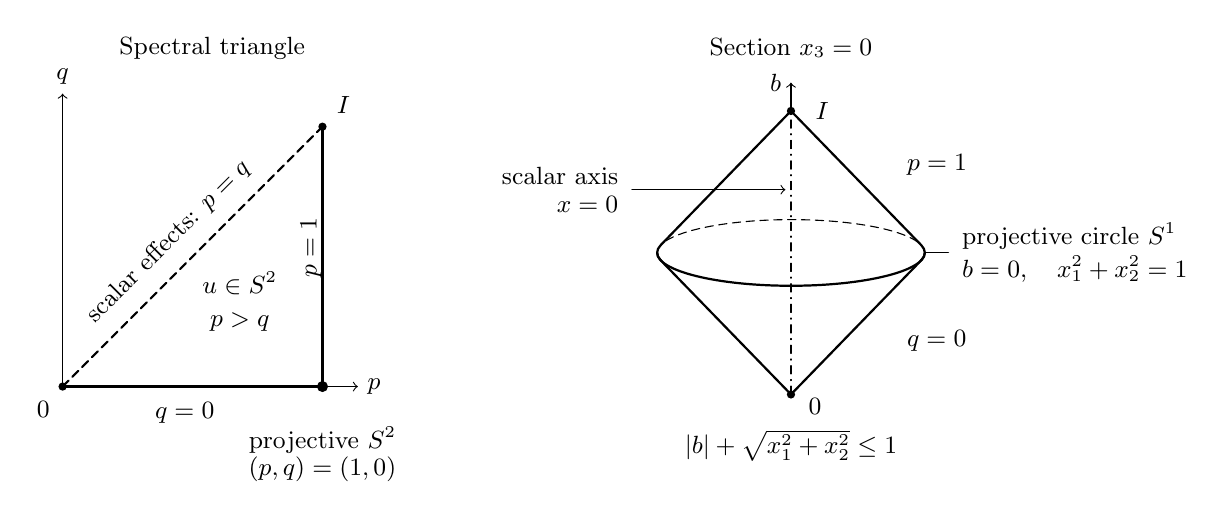
\begin{tikzpicture}[x=1cm,y=1cm,line cap=round,line join=round,
                    font=\small]
  % Left panel: exact ordered spectral triangle.
  \node at (1.9,4.30) {Spectral triangle};
  \draw[->,thin] (0,0) -- (3.75,0) node[right] {$p$};
  \draw[->,thin] (0,0) -- (0,3.72) node[above] {$q$};
  \draw[thick] (0,0) -- (3.3,0) -- (3.3,3.3);
  \draw[thick,densely dashed] (0,0) -- (3.3,3.3);
  \node[rotate=45,anchor=south] at (1.53,1.65)
    {scalar effects: $p=q$};
  \node[anchor=north] at (1.55,-0.08) {$q=0$};
  \node[rotate=90,anchor=south] at (3.41,1.77) {$p=1$};
  \node[align=center] at (2.25,1.08) {$u\in S^2$\\[1pt]$p>q$};
  \fill (0,0) circle (1.5pt);
  \fill (3.3,3.3) circle (1.5pt);
  \fill (3.3,0) circle (2pt);
  \node[anchor=north east] at (-0.04,-0.06) {$0$};
  \node[anchor=south west] at (3.36,3.34) {$I$};
  \node[anchor=north,align=center] at (3.30,-0.39)
    {projective $S^2$\\[-1pt]$(p,q)=(1,0)$};

  % Right panel: a three-dimensional section, shown in linear projection.
  % In local coordinates the map is
  % (x_1,x_2,b) -> (1.70*x_1,0.42*x_2+1.80*b).
  % The cone silhouette meets the projected unit circle at its exact
  % tangency points: sin(alpha)=0.42/1.80=7/30.
  \begin{scope}[shift={(9.25,1.70)}]
    \node at (0,2.60) {Section $x_3=0$};
    \pgfmathsetmacro{\tangentangle}{asin(7/30)}
    \pgfmathsetmacro{\tangentx}{1.70*cos(\tangentangle)}
    \pgfmathsetmacro{\tangenty}{0.42*sin(\tangentangle)}

    \draw[thin,densely dashed] (1.70,0)
      arc[start angle=0,end angle=180,x radius=1.70,y radius=0.42];
    \draw[thick] (-1.70,0)
      arc[start angle=180,end angle=360,x radius=1.70,y radius=0.42];
    \draw[thick] (-\tangentx,\tangenty) -- (0,1.80)
      -- (\tangentx,\tangenty);
    \draw[thick] (-\tangentx,-\tangenty) -- (0,-1.80)
      -- (\tangentx,-\tangenty);
    \draw[thick] (\tangentx,-\tangenty)
      arc[start angle=-\tangentangle,end angle=\tangentangle,
          x radius=1.70,y radius=0.42];
    \draw[thick] (-\tangentx,\tangenty)
      arc[start angle=180-\tangentangle,end angle=180+\tangentangle,
          x radius=1.70,y radius=0.42];

    \draw[thin,dash dot] (0,-1.80) -- (0,1.80);
    \draw[->,thin] (0,1.80) -- (0,2.16) node[left] {$b$};
    \fill (0,1.80) circle (1.5pt);
    \fill (0,-1.80) circle (1.5pt);
    \node[anchor=west] at (0.19,1.80) {$I$};
    \node[anchor=north west] at (0.10,-1.73) {$0$};
    \node[anchor=east,align=right] at (-2.07,0.80)
      {scalar axis\\[-1pt]$x=0$};
    \draw[->,thin] (-2.02,0.80) -- (-0.07,0.80);
    \node[anchor=west] at (1.35,1.12) {$p=1$};
    \node[anchor=west] at (1.35,-1.12) {$q=0$};
    \draw[thin] (1.71,0) -- (2.00,0);
    \node[anchor=west,align=left] at (2.05,0)
      {projective circle $S^1$\\[1pt]$b=0,\quad x_1^2+x_2^2=1$};
    \node[anchor=north] at (0,-2.13)
      {$|b|+\sqrt{x_1^2+x_2^2}\le1$};
  \end{scope}
\end{tikzpicture}
\caption{The four-dimensional effect body $|b|+|x|\le1$.
Each point of the spectral triangle with $p>q$ carries a direction
$u\in S^2$; on the scalar diagonal all directions represent the same
effect. The boundary pieces $q=0$ and $p=1$ meet at the projective stratum
$(p,q)=(1,0)$, which carries the full sphere $S^2$.
The right panel is a projection of the three-dimensional section
$x_3=0$; its equatorial circle is the intersection of that sphere
with the section.}
\label{fig:effectbody76}
\end{figure}

\section{The description entropy of all binary qubit effects}\label{sec:biasedentropy75}
Let
\[
 \mathfrak E=\{E=E^*\in\C^{2\times2}:0\le E\le I\}.
\]
An effect $E$ specifies the ordered measurement with effects $E,I-E$.
Write $\mathcal C_N(\mathfrak E,\delta)$ for its covering number under
$d_N$, allowing arbitrary legal memoryless centres of this interface,
and write $\mathcal C_N^{\mathrm{rat}}(\mathfrak E,\delta)$ when the
centres have rational Cartesian coordinates. Both eigenvalues and the
eigenspaces are charged. The spectral representation
$E=pP_u+q(I-P_u)$, $p\ge q$, represents a scalar effect only once,
independently of $u$.

\begin{theorem}[The full effect body]\label{thm:biasedcover75}
There are absolute constants $c,C,\delta_0>0$ such that, for every integer
$N\ge1$ and $0<\delta\le\delta_0$,
\begin{equation}\label{eq:biasedcover75}
 cN^2\log(N+2)\,\delta^{-4}
 \le \mathcal C_N(\mathfrak E,\delta)
 \le \mathcal C_N^{\mathrm{rat}}(\mathfrak E,\delta)
 \le CN^2\log(N+2)\,\delta^{-4}.
\end{equation}
Consequently the optimum fixed-length reusable payload is
\begin{equation}\label{eq:biasedbits75}
 2\log_2N+\log_2\log(N+2)+4\log_2(1/\delta)+O(1).
\end{equation}
The constants are uniform over the whole closed effect body, including
scalar, deterministic and projective effects. For rational accuracy
input, rational target data admit an exact rational encoder attaining
this order.
\end{theorem}
The logarithm records accumulation near the projective stratum, where
both outcome probabilities can approach their support endpoints.
We prove the upper bound by a finite rational construction and the
lower bound by separated families of projective-corner boxes.

\subsection{A rational spectral and angular code}
For $N\ge1$ and rational $0<\delta\le1/4$, put
\begin{equation}\label{eq:biasedspectralgrid75}
 B=\left\lceil\sqrt{64N/\delta^2}\right\rceil,\qquad
 s_i=\begin{cases}
 \displaystyle\frac{i^2}{B^2+i^2},&0\le i\le B,\\[2mm]
 \displaystyle1-\frac{(2B-i)^2}{B^2+(2B-i)^2},&B<i\le2B.
 \end{cases}
\end{equation}
Thus $0=s_0<s_1<\cdots<s_{2B}=1$. For $0\le j<i\le2B$ define
\begin{equation}\label{eq:biasedangulargrid75}
 K_{ij}^2=
 \frac{N(s_i-s_j)^2}
 {s_i(1-s_i)+s_j(1-s_j)+N^{-1}},\qquad
 A_{ij}=\max\left\{1,
      \left\lceil\sqrt{256K_{ij}^2/\delta^2}\right\rceil\right\}.
\end{equation}
Use the six signed stereographic charts
\begin{equation}\label{eq:biasedsphere75}
 u_a=\epsilon\frac{1-|z|^2}{1+|z|^2},\qquad
 u_b=\frac{2z_b}{1+|z|^2}\quad(b\ne a),\qquad
 a\in\{1,2,3\},\quad \epsilon\in\{-1,1\},
\end{equation}
with $z\in\{-A_{ij},\ldots,A_{ij}\}^2/A_{ij}$ for the spectral
pair $(s_i,s_j)$. Every chart word decodes to
$s_iP_u+s_j(I-P_u)$. A diagonal pair $i=j$ has the single word
$s_iI$. The exact number of words, including redundant chart words,
is
\begin{equation}\label{eq:biasedcapacity75}
 L_{N,\delta}=(2B+1)+
       \sum_{0\le j<i\le2B}6(2A_{ij}+1)^2.
\end{equation}

\begin{theorem}[Exact rational realization]\label{thm:biasedcodec75}
The words in \eqref{eq:biasedcapacity75} form a radius-$\delta/2$
cover of $\mathfrak E$ by legal rational effects, and
\begin{equation}\label{eq:biasedcapacitybound75}
 L_{N,\delta}\le C N^2\log(N+2)\,\delta^{-4}
\end{equation}
for an absolute $C$. If
\[
 E=\tfrac12\bigl((1+b)I+x\cdot\sigma\bigr),\qquad
 b\in\Q,\quad x\in\Q^3,\quad |b|+|x|\le1,
\]
then a covering word is computable by rational arithmetic and integer
comparisons. Its payload is one fixed-length index in the set of
\eqref{eq:biasedcapacity75}.
\end{theorem}
\begin{proof}
Write $f(t)=t^2/(1+t^2)$, $0\le t\le1$. For a probability in
$[0,1/2]$, round its inverse coordinate $t$ to the nearest multiple
of $1/B$; for a probability in $[1/2,1]$, use the reflected chart
$1-f(t)$. Choose the multiple of smaller magnitude at ties. This
defines a nondecreasing quantizer on $[0,1]$, so separately quantizing
$p\ge q$ preserves their order.

The square-root vector associated with $f(t)$ is
$(t,1)/\sqrt{1+t^2}$; its derivative has norm $1/(1+t^2)\le1$.
The reflected chart has the same bound. Hence the Euclidean
square-root distance between each probability and its quantization
is at most $1/(2B)$. If $H$ is this distance, the product-fidelity
inequality gives unhalved distance at most $2\sqrt N H$ between the
corresponding $N$-fold Bernoulli laws. The common two-coin programme
in Lemma~\ref{lem:spectralprojection75} therefore gives a spectral error
at most
\[
                         2\sqrt N/B\le\delta/4.
\]
This argument includes adaptive testers and entangled references.

If the quantized eigenvalues coincide, this completes the encoding.
Otherwise choose a signed chart whose distinguished coordinate has
maximal absolute value in the target direction. Its inverse coordinate
belongs to $[-1,1]^2$. Rounding its two coordinates to the grid of
denominator $A_{ij}$ gives angular error at most $2\sqrt2/A_{ij}$,
since geodesic distance is bounded by the length of the mapped
straight segment and the differential of stereographic projection has
norm at most two. The angular upper bound in Theorem~\ref{thm:biasedangular75}
gives error at most
\[
 \sqrt2 K_{ij}\frac{2\sqrt2}{A_{ij}}
                   \le\delta/4.
\]
The triangle inequality proves the covering assertion. Formula
\eqref{eq:biasedsphere75} preserves the unit sphere exactly, so every
decoded effect is legal and rational.

We verify exact computability even when the input eigenvalues are
irrational. Put $Q=|x|^2\in\Q$. The eigenvalues are
$(1+b\pm\sqrt Q)/2$. Each decision in the spectral rounding compares
one of these numbers with a rational threshold $f((k+1/2)/B)$ or its
reflection. Such a comparison is the sign of a rational number plus
or minus $\sqrt Q$; checking signs before squaring makes it an exact
rational comparison. If $Q=0$, the two quantized eigenvalues coincide.
Otherwise choose the smallest index $a$ maximizing $|x_a|$ and put
$\epsilon=\operatorname{sgn}(x_a)$. The inverse chart is
\[
                    z_b=\frac{x_b}{\sqrt Q+|x_a|}\quad(b\ne a).
\]
Its comparison with any rational rounding threshold again reduces
to the sign of a rational number plus a rational multiple of
$\sqrt Q$. The integers $B,A_{ij}$ are computed by integer squaring
and rational comparison. Thus no irrational normalization is required.
The decoder uses only the displayed rational formulae.

It remains to count the words. Set $m_i=\min(i,2B-i)$ and
$U=B^2/N$. Directly from \eqref{eq:biasedspectralgrid75},
\[
 \frac{m_i^2}{4B^2}\le s_i(1-s_i)\le\frac{m_i^2}{B^2},\qquad
 K_{ij}^2\le
          \frac{4NB^2}{m_i^2+m_j^2+U}.
\]
Each value of $m_i$ occurs at most twice. Since
$(2A_{ij}+1)^2\le C(1+K_{ij}^2/\delta^2)$, we obtain
\begin{equation}\label{eq:biasedlattice75}
 L_{N,\delta}\le CB^2+
 \frac{CNB^2}{\delta^2}
       \sum_{a,b=0}^{B}\frac1{a^2+b^2+U}.
\end{equation}
Here $U\ge1$. The part with $\max(a,b)\le\sqrt U$ is bounded by an
absolute constant. Each successive dyadic square ring contributes
at most another absolute constant. There are at most
$C\log(N+2)$ such rings, because $B/\sqrt U=\sqrt N$. Consequently
\[
              \sum_{a,b=0}^{B}\frac1{a^2+b^2+U}
                       \le C\log(N+2).
\]
Finally $B^2\le CN/\delta^2$, so \eqref{eq:biasedlattice75} proves
\eqref{eq:biasedcapacitybound75}. The support cutoff in the denominator
is retained throughout the count, including the endpoint grid words.
\end{proof}

\subsection{Packing the projective corner}
\begin{proof}[Proof of Theorem~\ref{thm:biasedcover75}]
The upper bound follows from Theorem~\ref{thm:biasedcodec75}. For a
real $\delta$, choose a rational $\delta'$ with
$\delta\le\delta'\le2\delta$ and use its radius-$\delta'/2$ code;
decrease $\delta_0$ to at most $1/8$. For the lower bound first let
$N\ge16$. For every
\[
                     t=8^j/N\le1/16,\qquad j\ge0,
\]
consider the effects with
\begin{equation}\label{eq:biasedcorner75}
 p=1-\alpha,\quad q=\beta,\quad
 t\le\alpha,\beta\le2t,\qquad
 u=u(z),\quad z\in[-1/4,1/4]^2,
\end{equation}
where $u(z)$ is the chart in \eqref{eq:biasedsphere75} with
$a=3,\epsilon=1$. On this square, spherical distance is bounded
above and below by absolute positive multiples of Euclidean distance
in $z$. Throughout \eqref{eq:biasedcorner75}, the eigenvalue gap is
at least $3/4$ and
\[
 p(1-p)\asymp q(1-q)\asymp t,\qquad
 p(1-p)+q(1-q)+N^{-1}\asymp t.
\]
The finite-distance comparison of Theorem~\ref{thm:biasedmetric75}
therefore supplies an absolute $c_1>0$ such that any two points in
this box satisfy
\begin{equation}\label{eq:biasedboxmetric75}
 d_N\ge c_1\min\left\{1,
       \sqrt{N/t}\,
       \bigl| (\alpha,\beta,z)-
              (\alpha',\beta',z')\bigr|_\infty\right\}.
\end{equation}
Choose an absolute sufficiently large $A$ and then an absolute
sufficiently small $\delta_0$. In each of the four coordinates take
a grid of spacing $A\delta\sqrt{t/N}$. Since $Nt\ge1$, this spacing
is at most half the width of either spectral interval when
$\delta\le\delta_0$. The resulting points have pairwise distance
at least $4\delta$ by \eqref{eq:biasedboxmetric75}, and their number
is at least
\[
 c\left(\frac{t}{\delta\sqrt{t/N}}\right)^2
   \left(\frac1{\delta\sqrt{t/N}}\right)^2
                         =cN^2\delta^{-4}.
\]

Points from different boxes are also uniformly separated. Indeed,
if $t'\ge8t$, then $\alpha'\ge t'$ and $\alpha\le2t\le t'/4$.
The spectral modulus of the corresponding upper eigenvalues is
bounded below by an absolute positive multiple of
$\sqrt{Nt'}\ge1$. The spectral noncancellation bound in
Theorem~\ref{thm:biasedmetric75} gives $d_N\ge c_2>0$.
Shrinking $\delta_0$ ensures that this is at least $4\delta$.
There are at least $c\log(N+2)$ permitted boxes. Their union is
therefore a $4\delta$-packing of cardinality
$cN^2\log(N+2)\delta^{-4}$.

For $1\le N<16$, use instead a fixed spectral rectangle
$5/8\le p\le3/4$, $1/4\le q\le3/8$ and the same angular chart.
Theorem~\ref{thm:biasedmetric75} gives a uniform local Euclidean lower
bound, and a grid of spacing $C\delta$ has at least $c\delta^{-4}$
points. The factor $N^2\log(N+2)$ is bounded on this finite range.
This proves the same lower estimate for all $N\ge1$.

A radius-$\delta$ ball about any legal centre contains at most one
point of a $4\delta$-packing, by the triangle inequality. Hence the
packing proves the lower bound with the stated centre convention.
Taking binary logarithms and rounding the index length proves
\eqref{eq:biasedbits75}.
\end{proof}

\subsection{The source of the logarithm}
The spectral and angular weights also give the following integral
form of the same accumulation. Put $v_p=p(1-p)$, $v_q=q(1-q)$ and
$\tau=N^{-1}$. Then
\begin{equation}\label{eq:biasedvolume75}
 \int_{0\le q\le p\le1}
 \frac{N^2(p-q)^2\,dp\,dq}
 {(v_p+v_q+\tau)\sqrt{(v_p+\tau)(v_q+\tau)}}
                         \asymp N^2\log(N+2).
\end{equation}
To verify this, near $p=1,q=0$ put $\alpha=1-p$, $\beta=q$.
After removing the factor $N^2$, the integrand is comparable to
\[
 \frac1{(\alpha+\beta+\tau)
             \sqrt{(\alpha+\tau)(\beta+\tau)}}.
\]
For $s=\alpha+\beta$, integration over $0\le\alpha\le s$ is
bounded above by an absolute constant times $1/(s+\tau)$.
For $s\ge2\tau$, restriction to $s/4\le\alpha\le3s/4$ gives the
matching lower bound. Integration in $s$ proves logarithmic growth.
Near the scalar endpoint $p=q=0$, the factor $(p-q)^2$ is at most
$(p+q)^2$, while $v_p+v_q\asymp p+q$; the remaining integral is
uniformly bounded. Complementation gives the same conclusion near
$p=q=1$. Away from these endpoint neighbourhoods,
$v_p+v_q$ is bounded below and the factors $v_p^{-1/2},v_q^{-1/2}$
are integrable. Bounded $N$ is absorbed into the constants.
Thus the extra logarithm is contributed by the projective corner.
The finite covering construction and packing above also include the
collapsed scalar coordinates, where the spectral representation
ceases to be a chart.

\section{Measurement discrimination, block resources, and learning}
\label{sec:matrixcomparison76}
\label{sec:blockcomparison78}
\label{sec:confidencecomparison80}

\subsection{Finite-use discrimination and horizontal geometry}
The measurement interface determines which discrimination results
apply.  Here the ordered classical outcome and an arbitrary external
reference are retained, while the device returns no postmeasurement
quantum system.  For projective measurements, Pucha\l a and
collaborators \cite[Corollary~1 and Theorem~2]{PPKKO72} give an
exact multiple-use formula with ancillary access, used in the
observable-readout theorem.  Fiur\'a\v sek--Mi\v cuda \cite{FM75}
study a restricted ancillary interface, with a different comparison
of adaptive and parallel probes.

For general POVMs, Krawiec--Pawela--Pucha\l a
\cite[Section~4]{KPP76} construct a pair of nine-outcome qutrit
rank-one measurements admitting perfect adaptive discrimination
with two calls and no perfect discrimination by any finite parallel
experiment.  Datta--Biswas--Saha--Augusiak
\cite[Theorems~3--5]{DBSA76} study entanglement-assisted single-use
discrimination, including perfect constructions and a qubit
entanglement advantage; their qubit construction has three outcomes.
These results concern retained-reference discrimination for broader
outcome alphabets.  For ordered binary effects,
\eqref{eq:matrixadaptivity76} bounds the adaptive advantage uniformly
in the horizon for each fixed input dimension.

The differential argument in Lemma~\ref{lem:matrixpath76} uses the
horizontal-gauge and channel-extension method
\cite{FI76,DKG67,DM76,KGAD76}.  Yuan--Fung give the parallel path
estimate \cite[Section~III, equation~(26), PDF version~3]{YF76},
and Sieniawski--Demkowicz-Dobrza\'nski integrate adaptive bounds
\cite[Section~IV.A]{SD76}.  The binary Sylvester choice produces
the regularized variance $M(I-M)$, whose path bound can be
integrated explicitly and matched by compressed nonadaptive tests.
Inverse-Sylvester expressions in Bures geometry
\cite{Dittmann76} and spectral matrix integration
\cite{SZGeom76} provide further antecedents.  Here the form acts on
the effect displacement $H$ with variance $V=M(I-M)$; the Bures
pullback under $M\mapsto V$ would instead act on the differential
$H-MH-HM$.  Theorem~\ref{thm:matrixcover76} combines the resulting
geometry with uniform operational-ball estimates and the nested
endpoint integral to obtain the binary-effect covering law.

\subsection{One-use tomography and acquisition resources}
Mele--Bittel \cite[Theorem~I.1]{MB67} give channel tomography with
$O(d_{\rm in}d_{\rm out}k\epsilon^{-2})$ calls at fixed confidence.
Their binary specialization
\cite[Lemmas~III.7--III.8 and Corollary~III.9]{MB67} returns a
legal effect with operator error at most $\epsilon$, using
\[
 M=1024d^2\epsilon^{-2}
   +O(d\epsilon^{-2}\log(1/\eta)),
 \qquad 4e^{-4d^2}<\eta<1,\quad 0<\epsilon<1.
\]
It prepares independent maximally entangled input--reference pairs
and processes the Choi copies collectively
\cite[Algorithm~I.2, Figure~1 and Section~III.2]{MB67}.  It
therefore belongs to the fresh-block class with $b=1$, which allows
coherent purification and collective output tomography.  The
source calls all invocations one parallel block; its inputs from
distinct invocations nevertheless remain independent.  Its
amplification \cite[Remark~III.4, equation~(165)]{MB67} gives
$O(d^2\epsilon^{-2}\log(1/\eta))$ calls for all
$0<\eta\le1/8$ with the same acquisitions.  The sharper confidence
extension derived below uses the dimension-dependent tail in the
printed Corollary~III.9.

Zambrano--Ramos-Calderer--Kueng
\cite[Definition~1 and Theorem~2]{ZRK76} use worst-input one-use
outcome total variation.  With $L$ outcomes, their global-$2$-design
protocol has sufficient budget
\[
 M\ge \frac{8(d^2+\epsilon(d^2+1)/6)}{\epsilon^2}
       \log\frac{2^{L+1}9^{2d}}{\eta}.
\]
It probes known inputs separately and returns a legal POVM by least
squares and projection.  Thus it also has $b=1$, without a retained
reference.  When $L=2$, its loss is $\|E-F\|_{\rm op}$, whereas
$d_1(E,F)=2\|E-F\|_{\rm op}$ in our normalization.  Their
Theorem~9 gives a constant-confidence lower bound
$\Omega((d^3+d^2L)\epsilon^{-2})$ for nonadaptive single-copy
measurements on known input states.

\subsection{Interior learning under the future-use loss}
Theorem~\ref{thm:interiorlearning78} applies the Mele--Bittel
binary estimator to $I/4\preceq E\preceq3I/4$ with
$\epsilon=\delta/(8\sqrt N)$ and $\eta=1/8$.  The horizontal
path estimate gives
\[
 d_N(E,F)\le4\sqrt N\|E-F\|_{\rm op}
 \qquad\text{when }\|E-F\|_{\rm op}\le1/8.
\]
Consequently $O(d^2N\delta^{-2})$ independent one-call probes
suffice at this confidence.  Theorem~\ref{thm:dimensionlower78}
gives the matching lower bound under arbitrary coherent adaptive
training.  This identifies the joint dimension, horizon, and
accuracy order on the stated interior.

For all integers $d,N\ge1$, $0<\delta\le2^{-13}$ and
$0<\eta\le1/8$, Theorem~\ref{thm:interiorconfidence80} gives
\[
 M^*_{\rm int}(d,N,\delta,\eta)
 =\Theta\!\left(N\delta^{-2}
             [d^2+d\log(1/\eta)]\right)
\]
with absolute constants.  The upper bound has $b=1$ and the lower
bound permits unrestricted coherent adaptive training.
Corollary~\ref{cor:operatorconfidence80} gives the corresponding
binary operator-learning order
$\Theta(\epsilon^{-2}[d^2+d\log(1/\eta)])$ for
$0<\epsilon\le2^{-14}$.

The upper bound uses the Mele--Bittel estimator with base failure
$q_d=2^{-3d}$, which satisfies $4e^{-4d^2}<q_d$ in their
Corollary~III.9.  Run it at a fixed fraction of the desired accuracy,
and repeat independently a number of times equal to the smallest
positive odd integer at least $2\log_2(1/\eta)/d$.  Metric-majority
selection and the binomial tail estimate then give
$O(\epsilon^{-2}[d^2+d\log(1/\eta)])$ calls for every
$0<\eta\le1/8$.  Lemma~\ref{lem:binaryconfidenceupper80}
records this confidence extension of the existing estimator.

For the confidence converse, Mele--Bittel's classicalisation of
diagonal multiple-coin channels
\cite[Lemma~IV.19 and Corollary~IV.20]{MB67} is a direct
antecedent.  Their corollary gives
$\Omega(d\epsilon^{-2}\log(d/\eta))$ for small operator error
and $0<\eta<1/4$.  Lemma~\ref{lem:diagonalconfidence80} gives a
null-versus-coordinate argument under the present coherent adaptive
interface and future-use loss.  Revealing the sampled diagonal
index isolates the hypothesis-dependent Bernoulli coin after a
common basis-dephasing map.  The classical--quantum relative-entropy
calculation permits different current quantum inputs under the
two hypotheses.  Summation of the testing inequalities gives
$\Omega(dN\delta^{-2}\log(1/\eta))$; its maximum with
Theorem~\ref{thm:dimensionlower78} is the asserted sum up to an
absolute factor.

Channel-learning converses have different domains.
Oufkir--Girardi \cite{OG67} and Chen--Zhang--Yu
\cite[Theorems~1.1 and~4.2]{CZY78} treat fully coherent channel
learning in one-use diamond loss.  The latter gives
$\Omega(rd_{\rm in}d_{\rm out}\epsilon^{-2})$ when
$rd_{\rm out}\ge2d_{\rm in}$ at constant confidence.  Quantum
output dimension two still allows nonclassical outputs, so that
general-channel theorem does not specialize directly to a
binary-qc converse.  For binary measurements, Mele--Bittel give
their projector packing \cite[Proposition~IV.17]{MB67} and the
diagonal-coin bound above.  The near-fair binary information
estimate in Lemma~\ref{lem:weakmeasurementinfo78} supplies the
self-contained growing-dimension converse used here.

\subsection{The closed body and independent acquisition blocks}
On the complete effect body, the hybrid inequality
\[
 d_N(E,F)\le2N\|E-F\|_{\rm op}
\]
converts both one-use tomography guarantees to sufficient budgets
$O_d(N^2\delta^{-2}\log(1/\eta))$.  Theorem~\ref{thm:blocklearning78}
and Corollary~\ref{cor:onecallseparation78} give the corresponding
acquisition obstruction: for fixed $d\ge2$, every fresh $b=1$
procedure learning the entire ordered binary effect body requires
\[
 M\ge cN^2\delta^{-2}\log(1/\eta).
\]
The converse allows classical adaptive choices, stored references,
their collective processing, and public bounded stopping.  It
therefore applies to every reconstruction from the acquisitions of
both cited tomography protocols.  The projective boundary forces
this full-body horizon order, while the interior calculation above
permits the linear order using the same acquisition resource.

More generally, for $d\ge2$, $1\le b\le N$,
$0<\delta\le\delta_*$ and $0<\eta\le1/8$,
Theorem~\ref{thm:blocklearning78} proves
\[
 c\frac{N^2}{b}\delta^{-2}\log(1/\eta)
 \le M_b^*(d,N,\delta,\eta)
 \le Cd^4\frac{N^2}{b}\delta^{-2}\log(d/\eta).
\]
Here $M_b^*$ is the worst-record budget for a common classical
estimate in the fresh-block model of
Section~\ref{sec:blocklearning78}.  Each block may use a reference
and adaptive quantum controls.  Stored outputs can be processed
jointly, but only the classical record determines the next fresh
probe; earlier quantum registers cannot feed its unfinished queries.
At $b=N$ this gives the fixed-dimensional linear-horizon order,
and at $b=1$ the quadratic-horizon order.  For $d=1$, the cost is
$\Theta(N\delta^{-2}\log(1/\eta))$ independently of $b$.

The all-confidence operator estimator gives a further full-body
upper bound.  Use Lemma~\ref{lem:binaryconfidenceupper80} at
$\epsilon=\delta/(2N)$, or use the block construction, selecting
the smaller public budget before acquisition.  This yields
\eqref{eq:fullbodyconfidenceupper80}:
\[
 M_b^*(d,N,\delta,\eta)
 \le C\frac{N^2}{\delta^2}
       \min\!\left\{d^2+d\log\frac1\eta,
                    \frac{d^4}{b}\log\frac d\eta\right\},
\]
for $d\ge2$, $1\le b\le N$,
$0<\delta\le\min\{2^{-13},\delta_*\}$ and
$0<\eta\le1/8$.  The lower and upper dimension dependences for
the complete body remain unmatched when the parameters grow jointly.

The block scale has established metrological antecedents.
Hyllus et al.\ \cite[Observation~1, equation~(9)]{Hyllus78} and
T\'oth \cite[Observation~3, equation~(6)]{Toth78} prove, for
$b$-producible qubit probes under linear phase encoding,
\[
 F_Q\le\lfloor M/b\rfloor b^2+
              (M-b\lfloor M/b\rfloor)^2\le Mb.
\]
Our block parameter also permits sequential controls within a fresh
block and concerns query acquisition rather than multipartite
entanglement of the final state.  The finite-pair fidelity argument
gives the confidence factor without an unbiasedness assumption.
Salek--Hayashi--Winter \cite[Section~II.2 and Section~V.2]{SHW68}
formulate classical feed-forward with arbitrary output quantum
memory and no input quantum memory, and study asymptotic
discrimination exponents.  Wilde et al.\
\cite[Proposition~21 and Appendix~B]{WBHK72} give adaptive
divergence converses and fidelity-to-error inequalities.
Section~\ref{sec:blocklearning78} establishes the finite-budget
conditional fidelity estimate with variable block lengths and
stopping.  Its upper bound blocks the future tester and applies the
common learner at the shorter horizon.

Restrictions on jointly measuring already supplied state copies
are a separate resource \cite{CLL78,NZ78}.  The fresh-query
restriction used here permits an unrestricted final joint
measurement.  Mele--Bittel's blockwise Choi processing
\cite[Section~I.5]{MB67} concerns the former resource.

The full-body common learner uses multiscale phase recovery
\cite{HB76,KLY76}, with a proved safe-angle induction, bias
cancellation, unknown-noise block selection, and conditional
confidence allocation.  Its matrix extension calibrates both
support endpoints and controls variance from data-selected
compressions before assembling a legal estimate.  These operations
provide one procedure at rank changes and repeated eigenvalues;
the pair-dependent witnesses of the metric proof serve only to
establish operational separation.

\subsection{Exact descriptions and finite collective synthesis}
Theorem~\ref{thm:matrixcodec77} gives an exact rational selection
rule with optimal fixed-dimensional payload on the closed body
in its small-error range.  Theorem~\ref{thm:interiorentropy79}
has explicit dimension-uniform constants on $[I/4,3I/4]$.
Its norm-ball volume argument and the Fano--Kraft proof of
Theorem~\ref{thm:prefixrate79} use standard geometric and
information-theoretic mechanisms to obtain the future-loss
description laws.  Theorem~\ref{thm:interiorlearnedcode79}
coarsens the Mele--Bittel estimator to a finite output and the exact
public dictionary without further device calls; its confidence
extension is Corollary~\ref{cor:interiorconfidencecode80}.

Computing the finite readout is a further question: measurable
finite coarsening alone does not give computable measurement
entries.  In Section~\ref{sec:effectivelearning80},
Lemma~\ref{lem:algebraicreadout80} expresses the risk on
independent Choi records by a first-order formula over the reals
with rational coefficients.  It includes positivity and
completeness of the conditional POVMs, the fixed dictionary, and
quantification over every real target in the interior.  Real
quantifier elimination decides feasibility; real-closed-field
transfer supplies an algebraic point, found by exact enumeration
and sign tests \cite[Theorems~2.77 and~2.80 and Chapter~14]{BPR80}.
An increasing search of the sample count terminates at the order
supplied by the statistical existence bound.  The resulting
Theorem~\ref{thm:effectiveinterior80} gives an algebraic readout
and finite trusted controls with
\[
 M=O(N\delta^{-2}[d^2+d\log(1/\eta)]),\qquad
 B=\tfrac12d^2\log_2N+d^2\log_2(1/\delta)+O(d^2).
\]

Section~\ref{sec:finiterisk81} gives finite rational certificates
for the same uniform risk.  If a fixed readout has failure at most
$\alpha$ on an operator-norm $r$-net for good-label radius $a$,
Theorem~\ref{thm:finitecertificate81} gives
\[
 \sup_{E\in\mathfrak I_d}
   \mathbb P_E\{\|E-C_J\|_{\rm op}>a+r\}\le\alpha+mr.
\]
The analytic input is
$\|\Gamma_m(E)-\Gamma_m(G)\|_1\le2m\|E-G\|_{\rm op}$.
For each nearby grid point $G$, one transfers its fixed set of good
labels between the two experiments; no continuity of label
selection is assumed.  With
$a=\delta/(8\lceil\sqrt N\rceil)$ and
$r\le\min\{\delta/(32\lceil\sqrt N\rceil),\eta/(16m)\}$,
exact grid inequalities at failure $\eta/4$ certify operational
error $5\delta/8$ with failure at most $5\eta/16$ for all real
interior effects.

Proposition~\ref{prop:rationalreadout81} mixes an arbitrary
$L$-outcome readout with the uniform outcome and rounds its first
$L-1$ effects at prescribed denominator
$Q=\lceil64L^2d^m/\eta\rceil$.  The last effect is their
complement, giving exact completeness; the mixing margin preserves
positivity.  The change of every output-index law is bounded by
$3\eta/32$.  A finite enumeration therefore contains a certified
rational readout whenever the statistical construction supplies the
required slack.  Exhausting this enumeration at each dyadic call
count gives Theorem~\ref{thm:rationallearner81} at the same joint
call and payload orders.  Only existence of the tomography readout
is used: its entries and continuous-outcome integrals are not
inputs to either synthesis.

Finite-control approximation charges the complete preparation and
classically conditioned readout instruments.  The pathwise total
unhalved error allowance $\eta$ changes index probabilities by at
most $\eta/2$, so the rational construction has actual failure at
most $13\eta/16<\eta$.  Acquisition remains fresh and one-call,
and the decoder returns the unchanged legal rational centre.
Neither construction requires coherent access to the device's
classical outputs or environment.  Rational verification replaces
real quantifier elimination in the latter construction, while both
separate device calls and payload from preprocessing, storage, and
known-control work.

Finite and efficient state tomography have substantial existing
constructions.  Pelecanos--Spilecki--Tang--Wright
\cite[Theorems~1.1--1.3, Section~3.3 and Figures~8--9]{PSTW80}
give an efficient purification reduction and efficient pure- and
mixed-state tomography; their Theorem~4.2 supplies discrete
approximate-design circuits used by the pure-state protocol.
Preserving the covariance and binary operator-error analysis of the
imported channel estimator under a different tomography
implementation requires an additional argument.  The constructions
here instead select a feasible collective readout with a uniform
future-loss guarantee and the exact public dictionary.  They prove
finite computability and, for the rational construction, finite
verifiability of the risk conditions.  Their exhaustive search,
dictionary reconstruction, workspace, and known-gate costs have no
efficiency bound.

\begingroup
\small
\setlength{\tabcolsep}{4pt}
\renewcommand{\arraystretch}{1.17}
\begin{longtable}{@{}>{\raggedright\arraybackslash}p{0.25\textwidth}>{\raggedright\arraybackslash}p{0.35\textwidth}>{\raggedright\arraybackslash}p{0.34\textwidth}@{}}
\toprule
Result and acquisition & Loss and parameter range & Training-call order\\
\midrule
\endfirsthead
\toprule
Result and acquisition & Loss and parameter range & Training-call order\\
\midrule
\endhead
Mele--Bittel with Lemma~\ref{lem:binaryconfidenceupper80};
independent Choi probes, $b=1$ &
Entire binary body; operator error $\epsilon$;
$0<\eta\le1/8$ &
$O(\epsilon^{-2}[d^2+d\log(1/\eta)])$;
source estimator with a confidence extension\\
Zambrano et al.; individual known probes, $b=1$ &
Binary global-design protocol; operator error $\epsilon$;
$0<\eta<1$ &
$O(d^2\epsilon^{-2}[d+\log(1/\eta)])$\\
Theorem~\ref{thm:interiorconfidence80}; independent Choi probes,
$b=1$ &
$I/4\preceq E\preceq3I/4$; future error $\delta$;
$d,N\ge1$, $0<\eta\le1/8$ &
$\Theta(N\delta^{-2}[d^2+d\log(1/\eta)])$;
coherent adaptive lower bound\\
Theorem~\ref{thm:effectiveinterior80}; synthesized algebraic
readout, $b=1$ &
Same interior and future loss; rational $\delta,\eta$ &
$O(N\delta^{-2}[d^2+d\log(1/\eta)])$;
finite trusted-control specification\\
Theorem~\ref{thm:rationallearner81}; certified rational readout,
$b=1$ &
Same interior and future loss; rational $\delta,\eta$ &
$O(N\delta^{-2}[d^2+d\log(1/\eta)])$;
finite rational risk certificate\\
Theorem~\ref{thm:blocklearning78}; fresh blocks of size $\le b$ &
Entire binary body; future error $\delta$;
$d\ge2$, $1\le b\le N$, $0<\eta\le1/8$ &
$\Theta_d((N^2/b)\delta^{-2}\log(1/\eta))$;
explicit upper bound in
\eqref{eq:fullbodyconfidenceupper80}\\
\bottomrule
\end{longtable}
\endgroup
The future-loss rows use the absolute small-error ranges stated in
their theorems.  The sharp joint dimension law applies to the
displayed interior, while the closed-body law is optimal in
horizon, accuracy, and confidence for fixed dimension.  The binary
consuming interface is common to the preceding table.  The next
subsection gives the separate finite-outcome interior analysis;
residual device quantum outputs are not covered by either family.


\subsection{Finite-outcome interiors and existing tomography}
Mele--Bittel's general channel theorem \cite[Theorem~III.3]{MB67}
already applies to channels with any finite classical output alphabet.
The present extension is not a claim that learning a multi-outcome
POVM is new.  Its constructive upper proof uses their binary
Corollary~III.9 through the confidence amplification and rational
realization in Sections~\ref{sec:confidencelearning80} and
\ref{sec:finiterisk81}.  For each label, the public randomization
$E_j\mapsto I_d/4+E_j/2$ supplies exactly the binary Choi record
required by that primitive.  The operator accuracy is
$\delta/(16k\lceil\sqrt N\rceil)$, not $\delta/N$.
The dimension-independent horizontal estimate supplies this improved
horizon conversion.  The lower theorem permits coherent adaptive
training and keeps its $d\log(1/\eta)$ term.

The general-outcome procedure of
Zambrano--Ramos-Calderer--Kueng \cite[Theorem~2]{ZRK76}
can also be evaluated directly under this future-use loss.
Their worst-input outcome total variation dominates each
$\|E_j-F_j\|_{\rm op}$: a single label is one of the events in the
total-variation supremum.  A finite legalization into
$\mathfrak P_{d,k}$ increases the maximum component error by at most
a constant factor, as in the proof of
Theorem~\ref{thm:multioutcomelearning82}.
Consequently their stated sufficient budget, with operator target
of order $\delta/(k\sqrt N)$, gives
\[
 O\!\left(k^2N\delta^{-2}d^2
                   [d+k+\log(1/\eta)]\right)
\]
calls in their independent known-input, no-retained-reference model.
This is a direct sufficient future-loss analysis of that estimator,
not a lower bound against it.  Its extra dimension factor is
consistent with its different acquisition model.  We neither infer
that every prior estimator requires the coarse $N^2$ substitution
nor claim that the displayed growing-$k$ bounds are minimax sharp.

The multi-outcome discrimination examples cited above concern
broader boundary families.  They are not contradicted by an
interior comparison under $E_j\succeq I_d/(2k)$.
The new tuple entropy uses its affine dimension $(k-1)d^2$ and a
norm-ball volume calculation.  It is not an extension of the binary
endpoint logarithmic law to an unanalysed multi-outcome boundary.
All comparisons here use the June 15, 2026 version of Mele--Bittel
and the published July 15, 2026 version of
Zambrano--Ramos-Calderer--Kueng.  An external human priority judgment
is separate from this author-side theorem comparison.

\appendix
% Verbatim self-contained prerequisite excerpt from sections/49-noisy-readout-crossover.tex.
% The complete section, including conditional-output results, remains in main.tex.
\section{A noise-uniform readout transition}\label{sec:noisyreadout73}
The dependence on the readout basis can change scale when noise approaches
an extremal measurement. We determine that transition in a fixed
one-dimensional family, without a positive spectral margin uniform in
the noise. The proof is a finite-distance argument; no conclusion is
inferred merely from a Fisher-information calculation.

Let $\sigma_1,\sigma_2$ be the first two Pauli matrices. For
$\theta\in\R/(2\pi\Z)$ and a public visibility $0\le\lambda\le1$, put
\begin{equation}\label{eq:noisyfamily73}
 E_{\theta,\lambda}^{\pm}
 =\frac12\bigl(I\pm\lambda(\cos\theta\,\sigma_1+
                                  \sin\theta\,\sigma_2)\bigr),\qquad
 \mathcal M_{\theta,\lambda}^{\pm}(X)=\tr(E_{\theta,\lambda}^{\pm}X).
\end{equation}
Both outcome labels are retained. The output quantum system is
one-dimensional. In particular, $\theta$ and $\theta+\pi$ are not
identified by an outcome relabelling. Let $h(\theta,\phi)\in[0,\pi]$
be circular distance and set
\begin{equation}\label{eq:noisyscale73}
 \eta=1-\lambda^2,\qquad
 K_{N,\lambda}=\lambda\sqrt{N\min\{N,\eta^{-1}\}},\qquad N\ge1,
\end{equation}
where $\eta^{-1}=+\infty$ at $\lambda=1$. Thus $K_{N,1}=N$ and
$K_{N,0}=0$. The visibility may depend arbitrarily on $N$ and the
requested error; it is not a target coordinate charged in this theorem.

Write $\mathcal C_{N,\lambda}(\delta)$ for the least number of legal
memoryless binary instruments of this interface whose $d_N$-balls of
radius $\delta$ cover all targets in \eqref{eq:noisyfamily73}.
Centres need not belong to the displayed family. Define
$\mathcal C^{\mathrm{rat}}_{N,\lambda}(\delta)$ by restricting centres
to family members with rational $\cos\theta,\sin\theta$; rational
visibility then gives rational effects. A constant in the following
statement is independent of all three parameters $N,\lambda,\delta$.

\begin{theorem}[Noise-uniform finite-use coding]\label{thm:noisycoding73}
For all $N\ge1$, $0\le\lambda\le1$, and all pairs of angles,
\begin{equation}\label{eq:noisymetric73}
 \frac1{64}\min\{1,K_{N,\lambda}h(\theta,\phi)\}
 \le d_N(\mathcal M_{\theta,\lambda},\mathcal M_{\phi,\lambda})
 \le\min\{2,K_{N,\lambda}h(\theta,\phi)\}.
\end{equation}
There are absolute $c,C>0$ such that, for $0<\delta\le2^{-10}$,
\begin{equation}\label{eq:noisycover73}
 c\left(1+\frac{K_{N,\lambda}}\delta\right)
 \le\mathcal C_{N,\lambda}(\delta)
 \le\mathcal C^{\mathrm{rat}}_{N,\lambda}(\delta)
 \le C\left(1+\frac{K_{N,\lambda}}\delta\right).
\end{equation}
Consequently the optimum fixed-length reusable payload is
\begin{equation}\label{eq:noisybits73}
 \log_2\left(1+\frac{K_{N,\lambda}}\delta\right)+O(1).
\end{equation}
The upper construction is an exact rational algorithm on rational
visibility, tolerance and unit-circle input coordinates. At $\lambda=0$
the family is a singleton and its optimum payload is zero.
\end{theorem}
The constants and the additive remainder are uniform up to the erased
and projective endpoints. In contrast, they do not assert an optimal
leading constant, a large-error coherent covering law, or a coding law
in which an unknown visibility is also encoded.

\subsection{A two-point programme with its noise dependence retained}
\begin{lemma}[An adaptive upper modulus]\label{lem:noisyupper73}
Let $h=h(\theta,\phi)$ and $a=\lambda\sin(h/2)$. If $\eta>0$, then
\begin{equation}\label{eq:noisyfiniteupper73}
 d_N(\mathcal M_{\theta,\lambda},\mathcal M_{\phi,\lambda})
 \le\min\left\{2,\ 2Na,\
             2\sqrt{1-\left(\frac{\eta}{\eta+a^2}\right)^N}\right\}.
\end{equation}
For $\eta=0$ the bound $\min\{2,2Na\}$ remains valid.
\end{lemma}
\begin{proof}
The difference of the two positive-outcome effects has operator norm
$a$. On a bipartite input state, the two output blocks of the difference
are $B$ and $-B$, where
$B=\tr_A[((E^+_{\theta,\lambda}-E^+_{\phi,\lambda})\otimes I)\rho]$.
Duality against Hermitian contractions gives $\|B\|_1\le a$.
An eigenstate of the effect difference attains equality. Hence
$d_1=2a$, including reference assistance. Replacing the calls one at a
time and using trace-norm contraction proves $d_N\le2Na$ for every
common adaptive tester.

Choose angle representatives with difference $h$ and let $u,v$ be the
unit vectors along their midpoint and its oriented perpendicular in
the equatorial plane. The two Bloch vectors are $m\pm av$, where
$m=\lambda\cos(h/2)u$. Put
$b=(1-\|m\|^2)^{1/2}=(\eta+a^2)^{1/2}$.
The two Bloch vectors $m\pm bv$ have norm one, so they define two legal
binary projective instruments, say $\mathcal A_+$ and $\mathcal A_-$.
The target pair is exactly the two mixtures of these same instruments
with programme laws
\[
 p_\pm=\bigl((1\pm t)/2,(1\mp t)/2\bigr),\qquad t=a/b.
\]
This construction depends on the pair, which is permissible in a
metric upper bound. It is not one fixed processor for the whole circle.

For a fixed tester, first supply $N$ independent programme bits and,
at each requested call, apply the indicated $\mathcal A_+$ or
$\mathcal A_-$. All subsequent operations, including the reference,
feedback and a stopping rule, are a common channel of these bits.
Unused bits are discarded. The root fidelity of $p_+,p_-$ is
$\sqrt{1-t^2}$. Purifying the classical laws and using contraction gives
\[
 \|p_+^{\otimes N}-p_-^{\otimes N}\|_1
 \le2\sqrt{1-(1-t^2)^N}.
\]
This also follows directly from the classical fidelity inequality.
Substitution proves \eqref{eq:noisyfiniteupper73}.
Finally $1-(1-t^2)^N\le Nt^2$ and $a\le\lambda h/2$ imply
\[
 d_N\le\min\{N\lambda h,\sqrt{N/\eta}\,\lambda h,2\}.
\]
The limiting projective bound is supplied by the hybrid estimate,
not by division by zero.
\end{proof}
Classical simulation by common extremal channels and the effect of
noise on the Heisenberg scale are established methods
\cite{DKG67}. Environment/programme-state processing under adaptive
use is also an established framework \cite{DW72,WBHK72,WW72}.
The point needed here is the exact two-point expression
\eqref{eq:noisyfiniteupper73} and its uniform conversion to a family
cover, rather than a new claim about the origin of those methods.

\subsection{Finite entangled blocks and a binary product estimate}
\begin{lemma}[Symmetric Bernoulli products]\label{lem:bernoullimajority73}
Let $P_\pm$ be Bernoulli laws with success probabilities
$(1\pm a)/2$, where $0\le a\le1$. For every integer $m\ge1$,
\begin{equation}\label{eq:bernoullimajority73}
 \|P_+^{\otimes m}-P_-^{\otimes m}\|_1
                   \ge\tfrac12\min\{1,a\sqrt m\}.
\end{equation}
\end{lemma}
\begin{proof}
Retain the largest odd number $r=2j+1\le m$ of coordinates, so
$r\ge m/2$. For their majority event write
$g_r(a)=P_+(\text{majority})-P_-(\text{majority})$.
Differentiating the finite binomial sum and cancelling consecutive
terms gives
\[
 g_r'(a)=r\binom{2j}{j}4^{-j}(1-a^2)^j.
\]
For $j\ge1$, the bound $\binom{2j}{j}4^{-j}\ge1/(2\sqrt j)$
follows by induction: the ratio of consecutive left sides is
$(2j+1)/(2j+2)\ge\sqrt{j/(j+1)}$. For
$0\le a\le r^{-1/2}$, Bernoulli's inequality gives
$(1-a^2)^j\ge1-j/r\ge1/2$. Thus
$g_r'(a)\ge\sqrt r/(2\sqrt2)$ on that interval. The case $r=1$
is immediate. Integration from zero and monotonicity yield
$g_r(a)\ge(2\sqrt2)^{-1}\min\{1,a\sqrt r\}$.
Unhalved distance is at least twice this event difference; using
$r\ge m/2$ proves the stated bound.
\end{proof}

\begin{lemma}[A noise-uniform pairwise witness]\label{lem:noisylower73}
The lower inequality in \eqref{eq:noisymetric73} is witnessed by
nonadaptive entangled blocks, each of at most $N$ qubits, followed by
classical parity and majority processing.
\end{lemma}
\begin{proof}
A block of $k$ inputs is prepared in
$(|0\rangle^{\otimes k}+e^{i\alpha}|1\rangle^{\otimes k})/\sqrt2$.
Multiplying the $k$ output signs of \eqref{eq:noisyfamily73} has mean
$\lambda^k\cos(k\theta-\alpha)$. This identity follows by applying
$\bigotimes_{i=1}^k(E^+-E^-)$ to the two off-diagonal terms of the
block density matrix. For the two hypotheses choose the one common
phase $\alpha=k(\theta+\phi)/2+\pi/2$. Their parity laws then have
opposite biases of magnitude
\begin{equation}\label{eq:ghzbias73}
                        a_k=\lambda^k|\sin(kh/2)|.
\end{equation}
Repeating $m=\lfloor N/k\rfloor$ independent blocks and ignoring
remaining calls is an admissible tester. Its unhalved output distance
is at least $\tfrac12\min\{1,\sqrt m\,a_k\}$ by
Lemma~\ref{lem:bernoullimajority73}. The phase and block size may depend
on the pair, but never on the unknown hypothesis or a private outcome.

Assume $\lambda>0$ and put
$T=\min\{N,\eta^{-1}\}$, $k_0=\lfloor T\rfloor$. Then
$T/2\le k_0\le T$. For every $1\le k\le k_0$,
\begin{equation}\label{eq:visibilityblock73}
                              \lambda^k\ge\lambda/2.
\end{equation}
Indeed, when $0<\eta<1$, the inequality
$\log(1-\eta)\ge-\eta/(1-\eta)$ and
$k-1\le\eta^{-1}-1$ give $(k-1)\log\lambda\ge-1/2$.
At $\eta=0$ the assertion is immediate.

If $h\le1/k_0$, choose $k=k_0$. Since
$\sin(kh/2)\ge kh/\pi$ and $m\ge N/(2k)$, we obtain
\[
 \sqrt m\,a_k\ge
 \frac{\lambda\sqrt{Nk_0}}{2\pi\sqrt2}h
 \ge\frac{K_{N,\lambda}}{4\pi}h.
\]
This gives a lower constant $1/(8\pi)$.
If $k_0=1$, use $k=1$ for all $h\le\pi$ instead. Now $T<2$
unless $T=1$, and $\sqrt N\lambda\sin(h/2)\ge
K_{N,\lambda}h/(\pi\sqrt2)$; this is stronger than required.

It remains that $k_0\ge2$ and $h>1/k_0$. Here
$\lambda\ge1/\sqrt2$. Choose $k=\max\{1,\lfloor1/h\rfloor\}$.
Then $k\le k_0$ and $1/2\le kh\le\pi$. Equations
\eqref{eq:ghzbias73} and \eqref{eq:visibilityblock73} give
$a_k\ge1/(4\pi\sqrt2)$. Even one such block has distance at least
$1/(8\pi\sqrt2)>1/64$. The three cases prove the claim.
For $\lambda=0$ both sides of the desired inequality vanish.
\end{proof}

\subsection{Covering and exact rational realization}
\begin{proof}[Proof of Theorem~\ref{thm:noisycoding73}]
The metric assertion follows from the preceding lemmas. For a lower
cover choose points on the circle with circular separation at least
$256\delta/K_{N,\lambda}$ whenever that quantity is at most $\pi$.
An equally spaced packing has at least a fixed constant times
$K_{N,\lambda}/\delta$ points. Every two points have $d_N$-distance
at least $4\delta$, because $256\delta\le1/4$.
No radius-$\delta$ ball, even about an arbitrary legal instrument, can
contain two such points. If the required angular separation exceeds
$\pi$, the trivial lower bound one suffices, with a smaller absolute
constant. This proves the first inequality in \eqref{eq:noisycover73}.

For the upper bound use the two rational semicircle charts
\begin{equation}\label{eq:circlechart73}
 z_s(t)=s\left(\frac{1-t^2}{1+t^2},\frac{2t}{1+t^2}\right),
                 \qquad s\in\{-1,1\},\quad -1\le t\le1.
\end{equation}
Each chart has angular speed $2/(1+t^2)\le2$. Round $t$ to the
nearest $j/B$, $-B\le j\le B$, with a fixed rule at ties. The
circular error is at most $1/B$. Thus any integer
$B\ge\max\{1,K_{N,\lambda}/\delta\}$ yields a cover with at most
$4B+2$ centres. For rational inputs, an entirely rational choice is
\begin{equation}\label{eq:noisygrid73}
 B=\max\left\{1,\min\left\{
   \left\lceil\frac{4N\lambda}{\delta}\right\rceil,
   \left\lceil\sqrt{\frac{16N\lambda^2}{\eta\delta^2}}\right\rceil
                                  \right\}\right\},
\end{equation}
omitting the second entry when $\eta=0$. Integer squaring and rational
comparison compute the ceiling square root exactly. Both entries are
ceilings of the corresponding real bounds, so their minimum is
$\lceil4K_{N,\lambda}/\delta\rceil$.
For $z=(x,y)$ on the rational unit circle choose $s=1$ when $x\ge0$
and $s=-1$ otherwise, and set $t=sy/(1+sx)$. Its denominator is at
least one, so it is rational and belongs to $[-1,1]$.

The chart digit $(s,j)$ determines a legal effect pair with eigenvalues
$(1\pm\lambda)/2$. No approximate positivity test, irrational
normalization or search over real angles is needed. A fixed-length
index over $4B+2$ slots includes the chart sign. Its length gives
\eqref{eq:noisybits73}. Redundant chart endpoints cause at most a
constant overhead. At $\lambda=0$ dispense with the chart and emit the
single fair, input-erasing measurement.
\end{proof}

\begin{corollary}[A continuous family of horizon exponents]\label{cor:noisyexponents73}
Fix $0<\delta\le2^{-10}$. If $\lambda_N\to1$ and
$1-\lambda_N^2=N^{-\alpha+o(1)}$ for $\alpha\ge0$, then
\[
 \frac{\log_2\mathcal C_{N,\lambda_N}(\delta)}{\log_2N}
                       \longrightarrow\frac{1+\min\{\alpha,1\}}2.
\]
If $\lambda_N=N^{-\beta+o(1)}\to0$, with $\beta\ge0$, the limit is
$\max\{1/2-\beta,0\}$. The projective and erased endpoints have
coefficients one and zero, respectively.
\end{corollary}
\begin{proof}
Substitute the two regimes in \eqref{eq:noisyscale73} and use
\eqref{eq:noisycover73}. The term $1+K/\delta$ handles a vanishing
or subpolynomial scale without taking the logarithm of zero.
\end{proof}

\begin{thebibliography}{99}
\bibitem{Watrous65} J. Watrous, \emph{The Theory of Quantum Information},
Cambridge University Press, 2018. Theorems~2.22 and~2.26
(Choi criteria), Corollary~3.40 (trace-norm contraction),
and Section~3.3, equation~(3.306) (hybrid comparison).
\bibitem{PLS66} T. Surawy-Stepney, J. Kahn, R. Kueng and M. Gu\c{t}\u{a},
Projected least-squares quantum process tomography,
\emph{Quantum} \textbf{6} (2022), 844;
arXiv:2107.01060v2, 18 October 2022.
\bibitem{Gutoski66} G. Gutoski,
On a measure of distance for quantum strategies,
\emph{J. Math. Phys.} \textbf{53} (2012), 032202;
arXiv:1008.4636v4, 14 March 2012.
\bibitem{NZGB67} S. G. Naik, M. Zartab, N. Gisin and M. Banik,
No-Go Theorem for Generic Simulation of Qubit Channels with Finite
Classical Resources, arXiv:2501.15807v2 (16 July 2025),
Theorems~2 and~5.
\bibitem{MB67} A. A. Mele and L. Bittel,
Optimal learning of quantum channels in diamond distance,
arXiv:2512.10214v3 (2026), Theorem~I.1, Lemmas~III.7--III.8,
Corollary~III.9 and Sections~III.1.1, IV.1.1.
\bibitem{OG67} A. Oufkir and F. Girardi,
Improved Lower Bounds for Learning Quantum Channels in Diamond
Distance, arXiv:2601.04180v4 (2026).
\bibitem{DKG67} R. Demkowicz-Dobrza\'nski, J. Ko\l ody\'nski
and M. Gu\c{t}\u{a}, The elusive Heisenberg limit in quantum-enhanced
metrology, \emph{Nature Communications} \textbf{3} (2012), 1063.
DOI: 10.1038/ncomms2067; arXiv:1201.3940v2, equations~(4)--(6)
(classical simulation), equations~(10)--(13) (channel extension),
and the classical-simulation argument in Methods.
\bibitem{YBCH68} Y.~Yang, G.~Bai, G.~Chiribella and M.~Hayashi,
Compression for quantum population coding,
\emph{IEEE Transactions on Information Theory} \textbf{64} (2018), no.~7,
doi:10.1109/TIT.2017.2788407;
arXiv:1701.03372v8.
\bibitem{SHW68} F.~Salek, M.~Hayashi and A.~Winter,
Usefulness of adaptive strategies in asymptotic quantum channel
 discrimination, \emph{Phys. Rev. A} \textbf{105} (2022), 022419;
arXiv:2011.06569v3 (17 March 2024).
\bibitem{CMW70} T.~Cooney, M.~Mosonyi and M.~M.~Wilde,
Strong converse exponents for a quantum channel discrimination problem
and quantum-feedback-assisted communication,
arXiv:1408.3373v3 (26 February 2016), p.~5 and Sections~4.1--4.2.
\bibitem{Acin70} A.~Ac\'in,
Statistical distinguishability between unitary operations,
\emph{Phys. Rev. Lett.} \textbf{87} (2001), 177901.
DOI: 10.1103/PhysRevLett.87.177901.
\bibitem{DFY70} R.~Duan, Y.~Feng and M.~Ying,
Entanglement is not necessary for perfect discrimination between
unitary operations, \emph{Phys. Rev. Lett.} \textbf{98} (2007), 100503.
DOI: 10.1103/PhysRevLett.98.100503.

\bibitem{DW72} S. Das and M. M. Wilde,
Quantum reading capacity: General definition and bounds,
\emph{IEEE Trans. Inform. Theory} \textbf{65} (2019), 7566--7583;
arXiv:1703.03706v3; doi:10.1109/TIT.2019.2929925.
\bibitem{WBHK72} M. M. Wilde, M. Berta, C. Hirche and E. Kaur,
Amortized channel divergence for asymptotic quantum channel discrimination,
\emph{Lett. Math. Phys.} \textbf{110} (2020), 2277--2336;
arXiv:1808.01498v2; doi:10.1007/s11005-020-01297-7.
\bibitem{WW72} X. Wang and M. M. Wilde,
Resource theory of asymmetric distinguishability for quantum channels,
\emph{Phys. Rev. Research} \textbf{1} (2019), 033169;
arXiv:1907.06306v2; doi:10.1103/PhysRevResearch.1.033169.
\bibitem{PPKKO72} Z. Pucha\l a, \L. Pawela, A. Krawiec, R. Kukulski and
M. Oszmaniec, Multiple-shot and unambiguous discrimination of von Neumann
measurements, \emph{Quantum} \textbf{5} (2021), 425;
arXiv:1810.05122v4; doi:10.22331/q-2021-04-06-425.


\bibitem{SZ74} M. Sedl\'ak and M. Ziman,
Optimal single-shot strategies for discrimination of quantum measurements,
\emph{Phys. Rev. A} \textbf{90} (2014), 052312;
arXiv:1408.0934; doi:10.1103/PhysRevA.90.052312.
Section VI, Example 4, equation (37).
\bibitem{PPKK74} Z. Pucha\l a, \L. Pawela, A. Krawiec and R. Kukulski,
Strategies for optimal single-shot discrimination of quantum measurements,
\emph{Phys. Rev. A} \textbf{98} (2018), 042103;
arXiv:1804.05856; doi:10.1103/PhysRevA.98.042103. Theorem 1.
\bibitem{FM75} J.~Fiur\'a\v sek and M.~Mi\v cuda,
Optimal two-copy discrimination of quantum measurements,
\emph{Phys. Rev. A} \textbf{80} (2009), 042312;
arXiv:0909.2940; doi:10.1103/PhysRevA.80.042312.

\bibitem{KPP76} A.~Krawiec, \L.~Pawela and Z.~Pucha\l a,
Discrimination of POVMs with rank-one effects,
\emph{Quantum Information Processing} \textbf{19} (2020), 428;
arXiv:2002.05452v1; doi:10.1007/s11128-020-02883-3.
\bibitem{DBSA76} C.~Datta, T.~Biswas, D.~Saha and R.~Augusiak,
Perfect discrimination of quantum measurements using entangled systems,
\emph{New Journal of Physics} \textbf{23} (2021), 043021;
arXiv:2012.07069v2; doi:10.1088/1367-2630/abecaf.
\bibitem{FI76} A.~Fujiwara and H.~Imai,
A fibre bundle over manifolds of quantum channels and its application
to quantum statistics,
\emph{J. Phys. A: Math. Theor.} \textbf{41} (2008), 255304;
doi:10.1088/1751-8113/41/25/255304. Theorems~4 and~5.
\bibitem{DM76} R.~Demkowicz-Dobrza\'nski and L.~Maccone,
Using entanglement against noise in quantum metrology,
\emph{Phys. Rev. Lett.} \textbf{113} (2014), 250801;
arXiv:1407.2934v3; doi:10.1103/PhysRevLett.113.250801.
\bibitem{KGAD76} S.~Kurdzia\l ek, W.~G\'orecki, F.~Albarelli
and R.~Demkowicz-Dobrza\'nski,
Using adaptiveness and causal superpositions against noise in quantum metrology,
\emph{Phys. Rev. Lett.} \textbf{131} (2023), 090801;
arXiv:2212.08106v2; doi:10.1103/PhysRevLett.131.090801.
\bibitem{YF76} H.~Yuan and C.-H.~F.~Fung,
Fidelity and Fisher information on quantum channels,
arXiv:1506.00819v3 (2017), Section~III, equation~(26).
\bibitem{SD76} S.~Sieniawski and R.~Demkowicz-Dobrza\'nski,
Adaptive quantum channel discrimination using methods of quantum metrology,
\emph{New Journal of Physics} \textbf{28} (2026), 024502;
arXiv:2510.15506v3; doi:10.1088/1367-2630/ae3edd.
\bibitem{Dittmann76} J.~Dittmann,
Explicit formulae for the Bures metric,
\emph{J. Phys. A: Math. Gen.} \textbf{32} (1999), 2663--2670;
doi:10.1088/0305-4470/32/14/007;
arXiv:quant-ph/9808044, entitled
\emph{Note on explicit formulae for the Bures metric}.
\bibitem{SZGeom76} H.-J.~Sommers and K.~\.{Z}yczkowski,
Bures volume of the set of mixed quantum states,
\emph{J. Phys. A: Math. Gen.} \textbf{36} (2003), 10083--10100;
arXiv:quant-ph/0304041v3; doi:10.1088/0305-4470/36/39/308.
\bibitem{ZRK76} L.~Zambrano, S.~Ramos-Calderer and R.~Kueng,
Fast quantum measurement tomography with optimal error bounds,
\emph{Quantum} \textbf{10} (2026), 2162;
arXiv:2507.04500v3; doi:10.22331/q-2026-07-15-2162.
\bibitem{BDPS76} A.~Bisio, G.~M.~D'Ariano, P.~Perinotti and M.~Sedl\'ak,
Quantum learning algorithms for quantum measurements,
\emph{Physics Letters A} \textbf{375} (2011), 3425--3434;
arXiv:1103.0480v2; doi:10.1016/j.physleta.2011.08.002.
\bibitem{HB76} B.~L.~Higgins, D.~W.~Berry, S.~D.~Bartlett,
M.~W.~Mitchell, H.~M.~Wiseman and G.~J.~Pryde,
Demonstrating Heisenberg-limited unambiguous phase estimation
without adaptive measurements,
\emph{New Journal of Physics} \textbf{11} (2009), 073023;
arXiv:0809.3308v4; doi:10.1088/1367-2630/11/7/073023.
\bibitem{KLY76} S.~Kimmel, G.~H.~Low and T.~J.~Yoder,
Robust calibration of a universal single-qubit gate set via robust phase estimation,
\emph{Phys. Rev. A} \textbf{92} (2015), 062315;
doi:10.1103/PhysRevA.92.062315;
erratum, \emph{Phys. Rev. A} \textbf{104} (2021), 069901,
doi:10.1103/PhysRevA.104.069901; arXiv:1502.02677v3.

\bibitem{Hyllus78} P.~Hyllus, W.~Laskowski, R.~Krischek,
C.~Schwemmer, W.~Wieczorek, H.~Weinfurter, L.~Pezz\'e and A.~Smerzi,
Fisher information and multiparticle entanglement,
\emph{Phys. Rev. A} \textbf{85} (2012), 022321;
arXiv:1006.4366v3; doi:10.1103/PhysRevA.85.022321.
Section~III.A, Observation~1, equation~(9).
\bibitem{Toth78} G.~T\'oth,
Multipartite entanglement and high-precision metrology,
\emph{Phys. Rev. A} \textbf{85} (2012), 022322;
arXiv:1006.4368v3; doi:10.1103/PhysRevA.85.022322.
Observation~3, equation~(6).
\bibitem{CZY78} K.~Chen, Z.~Zhang and N.~Yu,
Optimal lower bound for quantum channel tomography in away-from-boundary regime,
arXiv:2601.10683v1 (15 January 2026), Theorems~1.1, 3.2 and~4.2.
\bibitem{CLL78} S.~Chen, J.~Li and A.~Liu,
An optimal tradeoff between entanglement and copy complexity for state tomography,
arXiv:2402.16353v1 (26 February 2024).
\bibitem{NZ78} A.~Nayak and X.~Zhou,
Optimal Low-Rank Quantum State Tomography with Bounded-Sample Joint Measurements,
arXiv:2609.10514v1 (9 September 2026), Theorems~1.1--1.2.

\bibitem{BPR80} S.~Basu, R.~Pollack and M.-F.~Roy,
\emph{Algorithms in Real Algebraic Geometry}, second edition,
Algorithms and Computation in Mathematics, vol.~10,
Springer, Berlin, Heidelberg, 2006;
doi:10.1007/3-540-33099-2.
Theorems~2.77 and~2.80 and Chapter~14.
\bibitem{PSTW80} A.~Pelecanos, J.~Spilecki, E.~Tang and J.~Wright,
Mixed state tomography reduces to pure state tomography,
arXiv:2511.15806v1 (19 November 2025).
Theorems~1.1--1.3 and~4.2, Section~3.3, Figures~8--9.

\end{thebibliography}

\end{document}
